%\requirepackage[l2tabu,orthodox]{nag}
\documentclass[11pt,oneside,article]{memoir}
% !TEX root = ./CCC_Note.tex

\usepackage{amsmath}
\usepackage{amsthm}
\usepackage{amsfonts}
\usepackage{amssymb}
\usepackage{mathtools}
%\usepackage{datetime}
\usepackage[T1]{fontenc}
\usepackage[sc]{mathpazo}
\linespread{1.05}
\usepackage{mathrsfs}
\usepackage{euscript}
%\usepackage{MnSymbol}
\usepackage{paralist}
\usepackage{todonotes}
\usepackage{makecell}
\usepackage{booktabs}
\usepackage{tikz}
\usetikzlibrary{cd}
\usepackage{hyperref}
\usepackage{tensor}

\usetikzlibrary{decorations.markings,arrows.meta,calc,fit,quotes}
\hypersetup{final}

\DeclareMathOperator{\id}{id}
\DeclareMathOperator{\dom}{dom}
\DeclareMathOperator{\cod}{cod}
\DeclareMathOperator{\dvert}{Vert}
\DeclareMathOperator{\Lax}{Lax}
\DeclareMathOperator{\Hom}{Hom}
\DeclareMathOperator{\Prof}{Prof}
\DeclareMathOperator{\MProf}{MProf}
\DeclareMathOperator{\Int}{Int}
\DeclareMathOperator{\Ob}{Ob}
\DeclareMathOperator{\Tr}{Tr}


\theoremstyle{plain}
\newtheorem{theorem}{Theorem}[section]
\newtheorem*{theorem*}{Theorem}
\newtheorem{proposition}[theorem]{Proposition}
\newtheorem{corollary}[theorem]{Corollary}
\newtheorem{lemma}[theorem]{Lemma}
\newtheorem*{lemma*}{Lemma}

\theoremstyle{definition}
\newtheorem{definition}[theorem]{Definition}
\newtheorem{exercise}{Exercise}[section]

\theoremstyle{remark}
\newtheorem{example}[theorem]{Example}
\newtheorem{remark}[theorem]{Remark}

\newcommand{\prodb}{\mathbin{\Pi}}
\newcommand{\iso}{\cong}

\newcommand{\cat}[1]{\mathscr{#1}}
\newcommand{\Cat}[1]{\mathbf{#1}}
%\newcommand{\hom}{\mathrm{hom}}
\newcommand{\twocat}[1]{\mathcal{#1}}
\newcommand{\dblcat}[1]{\mathbb{#1}}
\newcommand{\btwo}{\mathbf{2}}
\newcommand{\FF}{\mathbb{F}\Cat{F}}
\newcommand{\FFD}{\FF(\dblcat{D})}
\newcommand{\Mon}{\Cat{Mon}}
\newcommand{\DMon}{\mathbb{M}\Cat{on}}
\newcommand{\Comon}{\Cat{Comon}}
\newcommand{\DComon}{\mathbb{C}\Cat{omon}}
\newcommand{\Bimon}{\Cat{Bimon}}
\newcommand{\Sq}{\mathbb{S}\Cat{q}}
\newcommand{\Span}{\mathbb{S}\Cat{pan}}
\newcommand{\Hor}{\twocat{H}or}
\newcommand{\LAdj}{\dblcat{L}\Cat{Adj}}
\newcommand{\RAdj}{\dblcat{R}\Cat{Adj}}
\newcommand{\MAdjC}{\Cat{MAdj}}
\newcommand{\MAdj}{\dblcat{M}\Cat{Adj}}
\newcommand{\EAdj}{\dblcat{E}\Cat{Adj}}
\newcommand{\SymMonCat}{\Cat{SymMonCat}}
\newcommand{\CompCat}{\Cat{CompCat}}
\newcommand{\Set}{\Cat{Set}}

\newcommand{\op}[1]{{#1}^{\text{op}}}
\newcommand{\vop}[1]{{#1}^{\text{vop}}}
\newcommand{\hop}[1]{{#1}^{\text{hop}}}

\newcommand{\Alg}{\mathrm{Alg}}
\newcommand{\Coalg}{\mathrm{Coalg}}
\newcommand{\RAlg}[1][]{\mathbb{R}_{#1}\text{-}\Alg}
\newcommand{\LCoalg}[1][]{\mathbb{L}_{#1}\text{-}\Coalg}
\newcommand{\LCoalgA}{\mathbb{L}_1\text{-}\Coalg}
\newcommand{\LCoalgB}{\mathbb{L}_2\text{-}\Coalg}

\newcommand{\twocell}[3][]{\arrow[draw=none,to path={(dom#2.center)--(cod#2.center)\tikztonodes}]{}[anchor=center,#1]{\Downarrow #3}}
\newcommand{\twocellalt}[3][]{\arrow[draw=none,to path={(dom#2.center)--(cod#2.center)\tikztonodes}]{}[anchor=center,#1]{#3}}
\newcommand{\twocellA}[2][]{\twocell[#1]{A}{#2}}
\newcommand{\twocellB}[2][]{\twocell[#1]{B}{#2}}
\newcommand{\twocellC}[2][]{\twocell[#1]{C}{#2}}
\newcommand{\twocellD}[2][]{\twocell[#1]{D}{#2}}
\newcommand{\twocellE}[2][]{\twocell[#1]{E}{#2}}
\newcommand{\twocellF}[2][]{\twocell[#1]{F}{#2}}

\tikzcdset{
	arrow style=tikz,
	diagrams={>={Classical TikZ Rightarrow[angle=63:4pt, line width=.6pt]}},
	arrows={semithick}
}

\tikzset{tick/.style={postaction={decorate,decoration={markings,mark=at position 0.5 with {\draw[-] (0,.4ex) -- (0,-.4ex);}}}}}
\tikzset{dom/.style={append after command={coordinate[alias=dom#1]}},
		domA/.style={dom=A}, domB/.style={dom=B},
		domC/.style={dom=C}, domD/.style={dom=D},
		domE/.style={dom=E}, domF/.style={dom=F}}
\tikzset{cod/.style={append after command={coordinate[alias=cod#1]}},
		codA/.style={cod=A}, codB/.style={cod=B},
		codC/.style={cod=C}, codD/.style={cod=D},
		codE/.style={cod=E}, codF/.style={cod=F}}


\tikzset{
	%label/.style={font=\everymath\expandafter{\the\everymath\scriptstyle}},
	wiring diagram/.style={
		every to/.style={out=0,in=180,draw},
		label/.style={
			font=\everymath\expandafter{\the\everymath\scriptstyle},
			inner sep=0pt,
			node distance=1pt and -2pt},
		semithick,
		node distance=1 and 1,
		decoration={markings, mark=at position .5 with {\arrow{stealth};}},
		ar/.style={postaction={decorate}},
		execute at begin picture={\tikzset{
			x=\bbx, y=\bby,
			every fit/.style={inner xsep=\bbx, inner ysep=\bby}}}
		},
	bbx/.store in=\bbx,
	bbx = 2cm,
	bby/.store in=\bby,
	bby = 1.75ex,
	bb port sep/.store in=\bbportsep,
	bb port sep=2,
	% bb wire sep/.store in=\bbwiresep,
	% bb wire sep=1.75ex,
	bb port length/.store in=\bbportlen,
	bb port length=4pt,
	bb min width/.store in=\bbminwidth,
	bb min width=.8cm,
	bb small/.style={bb port sep=1, bb port length=2.5pt, bbx=.4cm, bb min width=.4cm, bby=.7ex},
	bb/.code 2 args={
		\pgfmathsetlengthmacro{\bbheight}{\bbportsep * (max(#1,#2)+1) * \bby}
		\pgfkeysalso{draw,minimum height=\bbheight,minimum width=\bbminwidth,outer sep=0pt,
			rounded corners=2pt,thick,
			prefix after command={\pgfextra{\let\fixname\tikzlastnode}},
			append after command={\pgfextra{\draw
				\ifnum #1=0{} \else foreach \i in {1,...,#1} {
					($(\fixname.north west)!{\i/(#1+1)}!(\fixname.south west)$) +(-\bbportlen,0) coordinate (\fixname_in\i) -- +(\bbportlen,0) coordinate (\fixname_in\i')}\fi
				\ifnum #2=0{} \else foreach \i in {1,...,#2} {
					($(\fixname.north east)!{\i/(#2+1)}!(\fixname.south east)$) +(-\bbportlen,0) coordinate (\fixname_out\i') -- +(\bbportlen,0) coordinate (\fixname_out\i)}\fi;
			}}}
	},
	bb name/.style={append after command={\pgfextra{\node[anchor=north] at (\fixname.north) {#1};}}}
}

\usetikzlibrary{arrows,calc,chains,matrix,positioning,scopes,snakes}

%Begin tikz macros
\def\blackbox#1#2#3#4#5{%(width,height), number inputs, number outputs, label, arrow length
  \pgfgetlastxy{\llx}{\lly}%assumes path has been set to a point representing the lower left corner of the box
  \path #1;
  \pgfgetlastxy{\w}{\h}
  \pgfmathsetlengthmacro{\urx}{\llx+\w}
  \pgfmathsetlengthmacro{\ury}{\lly+\h}
  \draw (\llx,\lly) rectangle (\urx,\ury);
  \pgfmathsetlengthmacro{\xave}{(\llx+\urx)/2}
  \pgfmathsetlengthmacro{\yave}{\ury-8}
  \node at (\xave,\yave) {#4};
  \pgfmathsetlengthmacro{\ydiff}{\ury-\lly}
  \pgfmathsetlengthmacro{\lstep}{\ydiff/(#2+1)}
  \pgfmathsetlengthmacro{\rstep}{\ydiff/(#3+1)}
  \ifnum #2=0{}\else{ 
   \foreach \l in {1,...,#2}{
    \draw [->] ($(\llx,\lly)+(-#5/2,0)+\l*(0,\lstep)$) -- ($(\llx,\lly)+(#5/2,0)+\l*(0,\lstep)$);}}\fi
  \ifnum #3=0{}\else{
   \foreach \r in {1,...,#3}{
    \draw [->] ($(\urx,\ury)+(-#5/2,0)-\r*(0,\rstep)$) -- ($(\urx,\ury)+(#5/2,0)-\r*(0,\rstep)$);}}\fi
}

\def\blackboxinners#1#2#3#4#5{%(width,height), number inputs, number outputs, label, arrow length
  \pgfgetlastxy{\llx}{\lly}%assumes path has been set to a point representing the lower left corner of the box
  \path #1;
  \pgfgetlastxy{\w}{\h}
  \pgfmathsetlengthmacro{\urx}{\llx+\w}
  \pgfmathsetlengthmacro{\ury}{\lly+\h}
  \draw (\llx,\lly) rectangle (\urx,\ury);
  \pgfmathsetlengthmacro{\xave}{(\llx+\urx)/2}
  \pgfmathsetlengthmacro{\yave}{\ury-8}
  \node at (\xave,\yave) {#4};
  \pgfmathsetlengthmacro{\ydiff}{\ury-\lly}
  \pgfmathsetlengthmacro{\lstep}{\ydiff/(#2+1)}
  \pgfmathsetlengthmacro{\rstep}{\ydiff/(#3+1)}
  \ifnum #2=0{}\else{ 
   \foreach \l in {1,...,#2}{
    \pgfmathsetlengthmacro{\newx}{\llx+#5*28.45274/2}
    \pgfmathsetlengthmacro{\newy}{\lly+\l*\lstep}
    \node at ($(\newx,\newy)+(-1.5,\l*12-\l*\lstep)$) {\tiny$(\pgfmathparse{\newx/28.45274}\pgfmathresult cm,\pgfmathparse{\newy/28.45274}\pgfmathresult cm)$};
    \draw [->] ($(\llx,\lly)+(-#5/2,0)+\l*(0,\lstep)$) -- ($(\llx,\lly)+(#5/2,0)+\l*(0,\lstep)$);}}\fi
  \ifnum #3=0{}\else{
   \foreach \r in {1,...,#3}{
    \pgfmathsetlengthmacro{\newx}{\urx-#5*28.45274/2}
    \pgfmathsetlengthmacro{\newy}{\ury-\r*\rstep}
    \node at ($(\newx,\newy)+(1.5,-\r*12+\r*\rstep)$) {\tiny $(\pgfmathparse{\newx/28.45274}\pgfmathresult cm,\pgfmathparse{\newy/28.45274}\pgfmathresult cm)$};
    \draw [->] ($(\urx,\ury)+(-#5/2,0)-\r*(0,\rstep)$) -- ($(\urx,\ury)+(#5/2,0)-\r*(0,\rstep)$);}}\fi
}

\def\blackboxouters#1#2#3#4#5{%(width,height), number inputs, number outputs, label, arrow length
  \pgfgetlastxy{\llx}{\lly}%assumes path has been set to a point representing the lower left corner of the box
  \path #1;
  \pgfgetlastxy{\w}{\h}
  \pgfmathsetlengthmacro{\urx}{\llx+\w}
  \pgfmathsetlengthmacro{\ury}{\lly+\h}
  \draw (\llx,\lly) rectangle (\urx,\ury);
  \pgfmathsetlengthmacro{\xave}{(\llx+\urx)/2}
  \pgfmathsetlengthmacro{\yave}{\ury-8}
  \node at (\xave,\yave) {#4};
  \pgfmathsetlengthmacro{\ydiff}{\ury-\lly}
  \pgfmathsetlengthmacro{\lstep}{\ydiff/(#2+1)}
  \pgfmathsetlengthmacro{\rstep}{\ydiff/(#3+1)}
  \ifnum #2=0{}\else{ 
   \foreach \l in {1,...,#2}{
    \pgfmathsetlengthmacro{\newx}{\llx-#5*28.45274/2}
    \pgfmathsetlengthmacro{\newy}{\lly+\l*\lstep}
    \node at ($(\newx,\newy)+(-1.5,\l*12-\l*\lstep)$) {\tiny$(\pgfmathparse{\newx/28.45274}\pgfmathresult cm,\pgfmathparse{\newy/28.45274}\pgfmathresult cm)$};
    \draw [->] ($(\llx,\lly)+(-#5/2,0)+\l*(0,\lstep)$) -- ($(\llx,\lly)+(#5/2,0)+\l*(0,\lstep)$);}}\fi
  \ifnum #3=0{}\else{
   \foreach \r in {1,...,#3}{
    \pgfmathsetlengthmacro{\newx}{\urx+#5*28.45274/2}
    \pgfmathsetlengthmacro{\newy}{\ury-\r*\rstep}
    \node at ($(\newx,\newy)+(1.5,-\r*12+\r*\rstep)$) {\tiny $(\pgfmathparse{\newx/28.45274}\pgfmathresult cm,\pgfmathparse{\newy/28.45274}\pgfmathresult cm)$};
    \draw [->] ($(\urx,\ury)+(-#5/2,0)-\r*(0,\rstep)$) -- ($(\urx,\ury)+(#5/2,0)-\r*(0,\rstep)$);}}\fi
}


\def\dashblackbox#1#2#3#4#5{%(width,height), number inputs, number outputs, label, arrow length
  \pgfgetlastxy{\llx}{\lly}%assumes path has been set to a point representing the lower left corner of the box
  \path #1;
  \pgfgetlastxy{\w}{\h}
  \pgfmathsetlengthmacro{\urx}{\llx+\w}
  \pgfmathsetlengthmacro{\ury}{\lly+\h}
  \draw [dashed] (\llx,\lly) rectangle (\urx,\ury);
  \pgfmathsetlengthmacro{\xave}{(\llx+\urx)/2}
  \pgfmathsetlengthmacro{\yave}{\ury-8}
  \node at (\xave,\yave) {#4};
  \pgfmathsetlengthmacro{\ydiff}{\ury-\lly}
  \pgfmathsetlengthmacro{\lstep}{\ydiff/(#2+1)}
  \pgfmathsetlengthmacro{\rstep}{\ydiff/(#3+1)}
  \ifnum #2=0{}\else{ 
   \foreach \l in {1,...,#2}{
    \draw [->] ($(\llx,\lly)+(-#5/2,0)+\l*(0,\lstep)$) -- ($(\llx,\lly)+(#5/2,0)+\l*(0,\lstep)$);}}\fi
  \ifnum #3=0{}\else{
   \foreach \r in {1,...,#3}{
    \draw [->] ($(\urx,\ury)+(-#5/2,0)-\r*(0,\rstep)$) -- ($(\urx,\ury)+(#5/2,0)-\r*(0,\rstep)$);}}\fi
}

\def\directarc#1#2{%left coordinate, right coordinate
  \path #1;
  \pgfgetlastxy{\lx}{\ly}
  \path #2;
  \pgfgetlastxy{\rx}{\ry}
  \pgfmathsetlengthmacro{\xave}{(\lx+\rx)/2}
  \draw #1 .. controls (\xave,\ly) and (\xave,\ry) .. #2;
}

\def\loopright#1#2#3{%upper coordinate, lower coordinate, stretch width
  \path #1;
  \pgfgetlastxy{\ux}{\uy}
  \path #2;
  \pgfgetlastxy{\lx}{\ly}
  \pgfmathsetlengthmacro{\maxx}{max(\ux,\lx)}
  \pgfmathsetlengthmacro{\farx}{\maxx+#3}
  \draw #1 .. controls (\farx,\uy) and (\farx,\ly) .. #2;
}

\def\loopleft#1#2#3{%upper coordinate, lower coordinate, stretch width
  \path #1;
  \pgfgetlastxy{\ux}{\uy}
  \path #2;
  \pgfgetlastxy{\lx}{\ly}
  \pgfmathsetlengthmacro{\minx}{min(\ux,\lx)}
  \pgfmathsetlengthmacro{\farx}{\minx-#3}
  \draw #1 .. controls (\farx,\uy) and (\farx,\ly) .. #2;
}

\def\fancyarc#1#2#3#4{%upper coordinate, lower coordinate, stretch width, max height adjust
  \path #1;
  \pgfgetlastxy{\ux}{\uy}
  \path #2;
  \pgfgetlastxy{\lx}{\ly}
  \pgfmathsetlengthmacro{\xave}{(\lx+\ux)/2}
%  \node at (\lx,\ly+20){\tiny $\pgfmathparse{\lx/28.45274}\pgfmathresult cm$,\hsp$\pgfmathparse{\ux/28.45274}\pgfmathresult cm$};
%  \node at (\xave,\ly+50){\tiny $\pgfmathparse{\xave/28.45274}\pgfmathresult cm$};
  \pgfmathsetlengthmacro{\yave}{(\ly+\uy)/2+#4}
  \loopleft{#1}{(\xave,\yave)}{#3}
  \loopright{#2}{(\xave,\yave)}{#3}
}

\def\delaynode#1{%coordinates
   \filldraw[black] #1 circle (2pt);
}

\def\activetikz#1{$$\begin{tikzpicture}#1\end{tikzpicture}$$}
\def\inactivetikz#1{\begin{center}\fbox{Tikz picture exists but is not being displayed}\end{center}}
%End tikz macros

\newcommand{\vinp}[1]{\overline{\inp{#1}}}
\newcommand{\voutp}[1]{\overline{\outp{#1}}}
%\newcommand{\inp}[1]{#1^{\textnormal{in}}}
%\newcommand{\outp}[1]{#1^{\textnormal{out}}}
\newcommand{\inp}[1]{#1^-}
\newcommand{\outp}[1]{#1^+}

% \def\bhline{\Xhline{2\arrayrulewidth}}
% \def\bbhline{\Xhline{2.5\arrayrulewidth}}
\def\alg{{\text \textendash}\Cat{Alg}}
\def\To{\xrightarrow}
\def\ul{\underline}
\def\List{\textnormal{List}}

\newcommand{\erase}[1]{{}}
\def\NN{\mathbb{N}}
\def\ss{\subseteq}


\settrims{0pt}{0pt} % page and stock same size
%\setlxvchars %calculate line length such that there are about 65 characters per line in \normalfont
%\settypeblocksize{*}{33pc}{*} % {height}{width}{ratio}
\settypeblocksize{*}{39pc}{*} % {height}{width}{ratio}
\setlrmargins{*}{*}{1} % {spine}{edge}{ratio}
%\setulmargins{*}{*}{1} % {upper}{lower}{ratio}, hight of typeblock fixed
\setulmarginsandblock{1in}{1in}{*} % height of typeblock computed
\setheadfoot{\onelineskip}{2\onelineskip} % {headheight}{footskip}
\setheaderspaces{*}{1.5\onelineskip}{*} % {headdrop}{headsep}{ratio}
\checkandfixthelayout

\setcounter{tocdepth}{2}
\setcounter{secnumdepth}{2}
\pagestyle{companion}
\linespread{1.15}
\renewcommand*{\chaptitlefont}{\bfseries\large}
\setsecheadstyle{\bfseries\large\raggedright}
\setsubsecheadstyle{\bfseries\raggedright}

\title{string diagrams for traced and compact categories are oriented 1-cobordisms}
\author{
   david i. spivak%
      \thanks{spivak and schultz were supported by afosr grant fa9550--14--1--0031, onr grant n000141310260, and nasa grant nnh13zea001n.}
   \and patrick schultz${}^*$%\footnotemark[1]
   \and dylan rupel
}
\date{\vspace{-3ex}}

\begin{document}
\tightlists
\firmlists

\maketitle
\begin{abstract}
   we give an alternate conception of string diagrams as labeled 1-dimensional oriented cobordisms,
   the operad of which we denote by $\lcob{\labset}$, where $\labset$ is the set of string labels.
   the axioms of traced categories are fully encoded by $\lcob{\labset}$ in the sense that there is
   an equivalence between $\lcob{\labset}$-algebras, for varying $\labset$ and traced categories
   with varying object set. the same holds for compact categories, the difference being in terms of
   variance in $\labset$. we also prove a substantial generalization of these fact which
   characterizes lax functors out of compact or traced categories. \\

   \noindent\textbf{keywords:} traced monoidal categories, compact closed categories, monoidal categories, lax functors, equipments, operads, factorization systems.
\end{abstract}

% \setcounter{tocdepth}{1}
% \tableofcontents*

\chapter{introduction}\label{chap:intro}

traced symmetric monoidal categories, hereafter \emph{traced categories}, have been used to model
processes with feedback~\cite{abramsky1} or operators with fixed points~\cite{pontoshulman}. a
graphical calculus for traced categories was developed by joyal, street, and
verity~\cite{joyalstreetverity}, in which string diagrams of the form
\begin{equation}\label{dia:string_diagram}
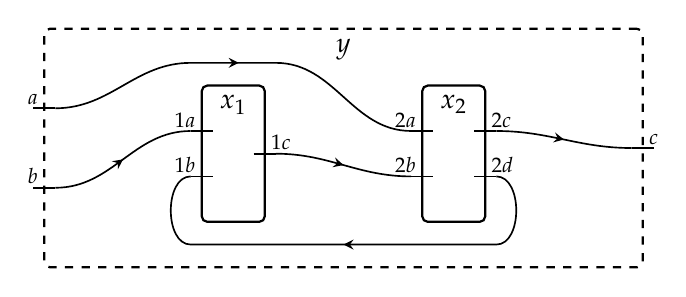
\begin{tikzpicture}[wiring diagram]
   \node[bb={2}{1}, bb name=$x_1$] (x1) {};
   \node[bb={2}{2}, right=of x1, bb name=$x_2$] (x2) {};
   \node[bb={2}{1}, dashed, fit={(x1) (x2) ($(x1.north)+(0,1.5)$) ($(x1.south)-(0,1)$)},
            bb name=$y$] (y) {};
   \draw[label]
      node[above left=of y_in1]     {$a$}
      node[above left=of y_in2]     {$b$}
      node[above right=of y_out1]   {$c$}
      node[above left=of x1_in1]    {$1a$}
      node[above left=of x1_in2]    {$1b$}
      node[above right=of x1_out1]  {$1c$}
      node[above left=of x2_in1]    {$2a$}
      node[above left=of x2_in2]    {$2b$}
      node[above right=of x2_out1]  {$2c$}
      node[above right=of x2_out2]  {$2d$};
   \draw[ar] (y_in2') to (x1_in1);
   \draw[ar] (x1_out1) to (x2_in2);
   \draw[ar] (x2_out1) to (y_out1');
   \draw[ar] let \p1=(x1.north west), \p2=(x1.north east), \n1={\y1+\bby}, \n2=\bbportlen in
      (y_in1') to (\x1-\n2,\n1) -- (\x2+\n2,\n1) to (x2_in1);
   \draw[ar] let \p1=(x2.south east), \p2=(x1.south west), \n1={\y1-\bby}, \n2=\bbportlen in
      (x2_out2) to[in=0] (\x1+\n2,\n1) -- (\x2-\n2,\n1) to[out=180] (x1_in2);
\end{tikzpicture}
\end{equation}
represent compositions. that is, new morphisms are constructed from old by specifying which outputs
will be fed back into which inputs. in fact, these are related to penrose diagrams in $\ncat{vect}$, and the word \emph{traced} originates in
this vector space terminology~\cite{joyalstreetverity}.

\section{traced string diagrams as cobordisms}\label{sec:traced_string_cob}

a string diagram usually does not explicitly include the outer box $y$. if we include it, as in
(\ref{dia:string_diagram}), the resulting \emph{wiring diagram} can be given another interpretation:
it represents a 1-dimensional cobordism between oriented 0-manifolds. for example, the box $x_1$ in
the picture includes only the data of a pair of finite sets,
$(\inp{x_1},\outp{x_1})=(\{1a,1b\},\{1c\})$, which can be interpreted as an oriented 0-manifold.
moreover, the wiring diagram itself, in which boxes $x_1,\ldots,x_n$ are wired together inside a
larger box $y$, can be interpreted as an oriented cobordism from $x_1\sqcup\cdots\sqcup x_n$ to $y$.
this is a morphism in the (colored) operad $\cob$, underlying the symmetric monoidal category of
oriented 1-cobordisms; see section~\ref{subsec:wds_and_cob}.

there is actually a bit more data in a string (or wiring) diagram for a traced category $\cat{c}$ than in a cobordism.
namely, each input and output of a box must be labeled by an object of $\cat{c}$ and the wires connecting boxes must respect the labels (e.g., in (\ref{dia:string_diagram}) object $2d$ must equal object $1b$). we will thus consider the operad $\lcob{\labset}$ of oriented 1-dimensional cobordisms over a fixed set $\labset$ of labels.

in the table below, we record these two interpretations of a string diagram. note the ``degree
shift'' between the second and third columns.
\begin{center}
\begin{tabular}{lll}
   \toprule
      \multicolumn{3}{c}{interpretations of string diagrams} \\
   \midrule
      string diagram & traced category $\cat{c}$ & $\lcob{\labset}$ \\
   \midrule
      wire label set, $\labset$ & objects, $\labset\coloneqq\ob(\cat{c})$ & label set, $\labset$ \\
      boxes, e.g., \tikz[wiring diagram,bb port sep=1,bby=2.4pt,bb min width=5.5pt,
                  bb port length=2pt,bb rounded corners=1pt,baseline=(b.south)]
               {\node[bb={1}{2}] (b) {};}
         & morphisms in $\cat{c}$& objects (oriented 0-mfds over $\labset$) \\
      string diagrams & compositions in $\cat{c}$& morphisms (cobordisms over $\labset$) \\
      nesting & axioms of traced cats & composition (of cobordisms) \\
   \bottomrule
\end{tabular}
\end{center}

\subsection{the formal connection between cob-algebras and traced categories}
   \label{subsec:statement_of_main_thm}

the relationship between these interpretations of string diagrams is most easily made precise when
the set $\labset$ of labels is fixed. let $\ttrcat$ denote the 2-category of traced categories,
strong traced functors, and monoidal natural isomorphisms \cite{hk}, and let $\trcat$ denote its
underlying 1-category.%
\footnote{
   we use a similar notational convention throughout this paper. we denote named 1-categories,
   monoidal categories, and operads with bold roman letters, e.g., $\ncat{cob}$, and unnamed
   1-categories with script, e.g., $\cat{c}$. for named 2-categories or bicategories we do almost
   the same, but change the font of the first letter to calligraphic, such as $\nncat{t}{rcat}$; for
   unnamed 2-categories we use (unbold) calligraphic, e.g., $\ccat{d}$. finally, for equipments
   (special double categories, see section~\ref{chap:background_equipments}) we make the first letter
   blackboard bold, whether named (e.g., $\ndcat{p}{rof}$) or unnamed (e.g., $\dcat{d}$). the
   objects in a category, 2-category, or double category will be denoted with the usual math font
   (e.g., $t\in\ob\trcat$).
}
finally, let $\trcat_{\labset}$ denote the subcategory in which the object set is fixed to be free
on the set $\labset$, together with identity-on-objects functors. for
any monoidal category $\cat{m}$, we denote by $\cat{m}\alg=\ncat{lax}(m,\set)$ the category of lax
functors $\cat{m}\to\set$. then there is an equivalence of categories
\begin{equation}\label{eq:single_fiber_tr}
   \lcob{\labset}\alg\equiv\trcat_{\labset}.
\end{equation}
some intuition for this statement will be given in section~\ref{subsec:cobalg_and_trcat}, and it
will be generalized in \ref{thm:theorema_statement} and proven as such in section~\ref{sec:deducing}.

\subsection{compact categories vs.\ traced categories}

for each of our main results about traced categories in this paper, we will also prove an analogous
result about compact closed symmetric monoidal categories, hereafter \emph{compact categories}. the
definition of compact category can be found in section~\ref{sec:compact_and_int}, or
in~\cite{maclane}. let $\ccompcat$ denote the 2-category of compact categories, and let $\compcat$
denote its underlying 1-category. as above, let $\compcat_{\labset}$ denote the subcategory of
compact categories whose object set is free on the set $\labset$ (so the objects are strings
$o_1o_2o_3^*$ of labels $o_i\in\labset$ and their formal duals, and the tensor product is
concatenation), together with identity-on-objects functors.

there is an equivalence of categories
\begin{equation}\label{eq:single_fiber_comp}
   \lcob{\labset}\alg\equiv\compcat_{\labset}.
\end{equation}
equations \eqref{eq:single_fiber_tr} and \eqref{eq:single_fiber_comp} and the relationship between them will be generalized in \ref{thm:theorema_statement}; see also \eqref{eqn:2pullbacks_1fiber}.

\section{the main results}\label{subsec:main_results}

the equivalence \eqref{eq:single_fiber_tr} (and likewise \eqref{eq:single_fiber_comp}) has two
drawbacks: the object set of the traced category is fixed, and it is assumed to be a free monoid; we
refer to this later condition using the term \emph{object-free}. much of the work in this paper is
to relax these two conditions. for the latter, we prove that the 2-category of traced categories is
equivalent to that of object-free traced categories (see corollary~\ref{cor:trcat_objectfree}). for
the former, we first explain what kind of variance is appropriate.

there are adjunctions
\begin{equation*}
   \adjoint{\set}{\trcat}{\ft}{\ut}
   \qquad
   \adjoint{\set}{\compcat}{\fc}{\uc}
\end{equation*}
which induce monads $\tt$ (respectively $\tc$) on $\set$. the monad $\tt$ is in fact isomorphic to
the free monoid monad, while $\tc$ is isomorphic to the free monoid-with-involution monad.

let $\cat{c}$ and $\cat{c}'$ be object-free traced categories, such that $\ob(\cat{c})$ is the free
monoid on a set $\labset$ and $\ob(\cat{c}')$ is the free monoid on a set $\labset'$. a strong
(traced) functor $f\colon \cat{c}\to \cat{c}'$ sends each object in $\labset$ to the tensor product
of finitely many objects in $\labset'$; that is, it induces a function $\ob
f\colon\labset\to\tt(\labset')$. let $\set_{\tt}$ denote the kleisli category of this monad, so $\ob
f$ is identified with a morphism in $\set_{\tt}$. likewise, if $\cat{c}$ and $\cat{c}'$ are
object-free compact categories, then the object part $\ob f$ of a strong functor
$f\colon\cat{c}\to\cat{c}'$ can be identified with a morphism in the kleisli category $\set_{\tc}$.

the compact category $\lcob{\labset}$ varies functorially in $\labset\in\set$, and we will see later
that this functor extends to functors
\begin{equation*}
   (\lcob{\bullet})\colon\set_{\tt}\to\compcat\qquad\tn{and}
   \qquad
   (\lcob{\bullet})\colon\set_{\tc}\to\compcat
\end{equation*}
(see~\eqref{dia:tmvsfrmoncat} and~\eqref{eqn:fmc}). we can compose these with $\lax(-,\set)$ to
obtain functors which we denote
\begin{equation}\label{eqn:cob/bullet}
   (\lcob{\bullet})\alg\colon\set_{\tt}^{\mathrm{op}}\too\cat,
   \qquad
   (\lcob{\bullet})\alg\colon\set_{\tc}^{\mathrm{op}}\too\cat.
\end{equation}
by applying the grothendieck construction to (\ref{eqn:cob/bullet}), we obtain fibrations for which
the fiber over $\labset$ is equivalent, using \eqref{eq:single_fiber_tr} and
\eqref{eq:single_fiber_comp}, to $\trcat_{\labset}$ and $\compcat_{\labset}$, respectively, for some
fixed label set $\labset$. our first main result says that the total categories of these fibrations
are \emph{almost} equivalent to the 2-category $\ttrcat$ and $\ccompcat$.

\begin{named}{theorem a}\label{thm:theorema_statement}
  there is a fully faithful functor of 1-categories
  \begin{equation}\label{eqn:tracedcobalg}
     \int^{\labset\in\set_{\tt}}(\lcob{\labset})\alg \to \trcat
  \end{equation}
  such that the induced 2-functor $\int^{\labset\in\set_{\tt}}(\lcob{\labset})\alg\to\ttrcat$ is
  2-essentially surjective.

  the above statements also hold when $\tt, \trcat$, and $\ttrcat$ are replaced by $\tc, \compcat$,
  and $\ccompcat$, respectively.
\end{named}

the proof of this result can be found in section~\ref{sec:deducing}.

\begin{remark}
   it would be too much to ask \eqref{eqn:tracedcobalg} to be an equivalence of 1-categories,
   because $\trcat$ throws away, rather than quotients by, natural isomorphisms in $\ttrcat$. on the
   other hand, we cannot expect algebras on $\lcob{\labset}$ to say anything about 2-cells, so the
   statement of \ref{thm:theorema_statement} is the best we can expect.

   another way of reading \ref{thm:theorema_statement} is that the grothendieck construction (the
   category on the left) is equivalent to the 1-category coskeleton of $\ttrcat$, that is, the
   1-category obtained from $\ttrcat$ by identifying naturally isomorphic traced functors.
\end{remark}

\begin{remark}
   the most naive way of handling variation of the label set $\labset$ is to use plain functions
   $\labset\to\labset'$. that is, instead of taking the grothendieck construction of the functors
   \eqref{eqn:cob/bullet}, we could use the most evident functor
   $\lax(\lcob{\bullet},\set)\colon\set\to\cat$. this would lead to a version of
   \ref{thm:theorema_statement} in which the right hand side is a 2-category of ``traced colored
   props''. we will not pursue this direction in this paper; however, the interested reader familiar
   with props should have no difficulty defining traced colored props and proving the analogue of
   \ref{thm:theorema_statement} as a corollary of our results. (for more on props, see
   e.g.~\cite{hackneyrobertson}.)
\end{remark}

\subsection{generalization: lax algebras on compact categories}

in the course of proving \ref{thm:theorema_statement}, we will also prove a more general result
which drops the restriction to object-free traced (and compact) categories.

we will see (\ref{thm:orthogonal} and \ref{prop:compprof_exact}) that there is a factorization
system on $\trcat$, and similarly on $\compcat$, in which the left class consists of
bijective-on-objects functors and the right class consists of fully faithful functors. let
$\trcat^{\bo}$ (resp.~$\compcat^{\bo}$) be the full subcategory of the arrow category $\trcat^{\to}$
(resp.~$\compcat^{\to}$) spanned by the bijective-on-objects functors.

using these factorization systems, we will see that the domain functors
$$\dom\colon\trcat^{\bo}\twoheadrightarrow\trcat,\qquad\dom\colon\compcat^{\bo}\twoheadrightarrow\compcat$$
are fibrations. for a fixed traced category $\cat{t}$, the fiber
$\trcat^{\bo}_{\cat{t}/}\coloneqq\dom^{-1}(\cat{t})$ is the category of strong, bijective-on-objects
functors from $\cat{t}$ to another traced category, with the evident commutative triangles as
morphisms, and likewise for $\compcat^{\bo}_{\cat{c}/}$ with $\cat{c}$ a compact category. note that
$\trcat_{\labset}\iso\trcat^{\bo}_{(\ft\labset)/}$, and similarly for $\compcat_{\labset}$.

recall from~\cite{joyalstreetverity} that traced categories can be thought of as full subcategories
of compact categories.  the int construction, applied to a traced category $\cat{c}$, returns the
smallest compact category $\int(\cat{c})$ of which it is a monoidal subcategory. we will recall these
notions in sections~\ref{sec:intuition_for_traced} and~\ref{sec:compact_and_int}.

generalizing \eqref{eq:single_fiber_tr} and \eqref{eq:single_fiber_comp}, we can give a complete
characterization of lax functors out of compact categories. for a fixed traced category $\cat{t}$
and a fixed compact category $\cat{c}$, there are equivalences of categories
\begin{equation}\label{eqn:lax_compcat_bo}
   \lax(\int(\cat{t}),\set)\equiv\trcat^{\bo}_{\cat{t}/},
   \qquad
   \lax(\cat{c},\set)\equiv\compcat^{\bo}_{\cat{c}/}.
\end{equation}
one advantage of this generalization is that it is more straightforward to handle varying the
categories $\cat{t}$ and $\cat{c}$. namely, we will prove in section~\ref{sec:deducing} the
following theorem:

\begin{named}{theorem b}\label{thm:theoremb_statement}
   there are equivalences of fibrations
   \begin{equation*}
      \begin{tikzcd}[column sep=-1em]
         \int\limits^{\mathclap{\cat{c}\in\trcat}} \lax(\int(\cat{c}),\set)
               \ar[rr,"\equiv"] \ar[dr,two heads]
            && \trcat^{\bo} \ar[dl,two heads,"\dom" pos=.4] \\
         & \trcat &
      \end{tikzcd}
      \qquad\quad
      \begin{tikzcd}[column sep=-1em]
         \int\limits^{\mathclap{\cat{c}\in\compcat}} \lax(\cat{c},\set)
               \ar[rr,"\equiv"] \ar[dr,two heads]
            && \compcat^{\bo} \ar[dl,two heads,"\dom" pos=.4] \\
         & \compcat &
      \end{tikzcd}
   \end{equation*}
\end{named}

we can give a better high-level story once we have reviewed \emph{equipments}; see the introduction
to section~\ref{chap:equipments_monoidal_profunctors}. for the remainder of the introduction, we
will attempt to build intuition.

\section{wiring diagrams, cobordisms, and traced categories}

in this section, we give a bit more intuition about the connection between wiring diagrams and
cobordisms, and the equivalence between the category of traced categories and the category of
cobordism algebras.

\subsection{wiring diagrams and $\cob$}\label{subsec:wds_and_cob}

the objects in $\cob$ are signed sets $(\inp{x},\outp{x})$, each of which can be drawn as a box with
input wires $\inp{x}$ drawn entering the box, on its left, and output wires $\outp{x}$ drawn exiting
the box, on its right. for the time being, we call the latter style \emph{an interface}.

\[
   \begin{tikzpicture}[node distance=0 and 0, baseline=(current bounding box.center)]
      \node (a1) {$-$};
      \node[below=-.1 of a1] (a2) {$-$};
      \node[below=-.1 of a2] (a3) {$-$};
      \node[below=-.1 of a3] (b1) {$+$};
      \node[below=-.1 of b1] (b2) {$+$};
   \end{tikzpicture}
   \hspace{4em}
   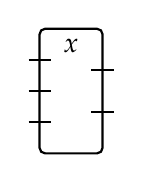
\begin{tikzpicture}[wiring diagram, bby=1.2ex, baseline=(current bounding box.center)]
      \node[bb={3}{2},bb name=$x$] {};
   \end{tikzpicture}
\]

wiring diagrams seem to be a new way to visualize morphisms in the symmetric monoidal category
$\cob$ of 1-dimensional oriented cobordisms. in fact, they are better suited to the operad
associated to $\cob$. the following shows the two approaches to drawing a 2-ary morphism $x_1,x_2\to
y$:

\[
   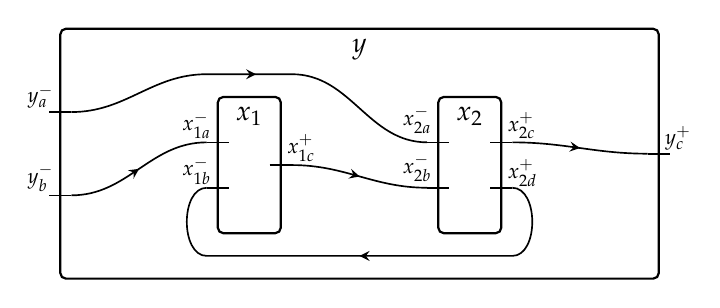
\begin{tikzpicture}[wiring diagram, baseline=(current bounding box.center)]
      \node[bb={2}{1}, bb name=$x_1$] (x1) {};
      \node[bb={2}{2}, right=of x1, bb name=$x_2$] (x2) {};
      \node[bb={2}{1}, fit={(x1) (x2) ($(x1.north)+(0,2)$) ($(x1.south)-(0,1)$)},bb name =$y$] (y) {};
      \draw[label]
          node[above left=of y_in1]     {$\inp{y}_a$}
          node[above left=of y_in2]     {$\inp{y}_b$}
          node[above right=of y_out1]   {$\outp{y}_c$}
          node[above left=1pt and -2pt of x1_in1]    {$\inp{x}_{1a}$}
          node[above left=1pt and -2pt of x1_in2]    {$\inp{x}_{1b}$}
          node[above right=1pt and -2pt of x1_out1]  {$\outp{x}_{1c}$}
          node[above left=3pt and -2pt of x2_in1]    {$\inp{x}_{2a}$}
          node[above left=2pt and -2pt of x2_in2]    {$\inp{x}_{2b}$}
          node[above right=1pt and -2pt of x2_out1]  {$\outp{x}_{2c}$}
          node[above right=0pt and -2pt of x2_out2]  {$\outp{x}_{2d}$};
      \draw[ar] (y_in2') to (x1_in1);
      \draw[ar] (x1_out1) to (x2_in2);
      \draw[ar] (x2_out1) to (y_out1');
      \draw[ar] let \p1=(x1.north west), \p2=(x1.north east), \n1={\y1+\bby}, \n2=\bbportlen in
          (y_in1') to (\x1-\n2,\n1) -- (\x2+\n2,\n1) to (x2_in1);
      \draw[ar] let \p1=(x2.south east), \p2=(x1.south west), \n1={\y1-\bby}, \n2=\bbportlen in
         (x2_out2) to[in=0] (\x1+\n2,\n1) -- (\x2-\n2,\n1) to[out=180] (x1_in2);
   \end{tikzpicture}
   \qquad
   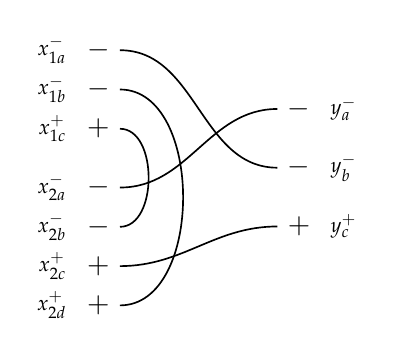
\begin{tikzpicture}[x=1cm,y=1ex,node distance=1 and 1,semithick,every label quotes/.style={font=\everymath\expandafter{\the\everymath\scriptstyle}},every to/.style={out=0,in=180},baseline=(current bounding box.center)]
      \node ["$\inp{x}_{1a}$" left] (x1a) {$-$};
      \node [below=0 of x1a, "$\inp{x}_{1b}$" left] (x1b) {$-$};
      \node [below=0 of x1b, "$\outp{x}_{1c}$" left] (x1c) {$+$};
      \node [below=1.5 of x1c, "$\inp{x}_{2a}$" left] (x2a) {$-$};
      \node [below=0 of x2a, "$\inp{x}_{2b}$" left] (x2b) {$-$};
      \node [below=0 of x2b, "$\outp{x}_{2c}$" left] (x2c) {$+$};
      \node [below=0 of x2c, "$\outp{x}_{2d}$" left] (x2d) {$+$};
      \node [below right=1.5 and 2 of x1a, "$\inp{y}_a$" right] (ya) {$-$};
      \node [below=1.5 of ya, "$\inp{y}_b$" right] (yb) {$-$};
      \node [below=1.5 of yb, "$\outp{y}_c$" right] (yc) {$+$};
      \draw (x1a) to (yb);
      \draw (x1b) to[in=0] (x2d);
      \draw (x1c) to[in=0] (x2b);
      \draw (x2a) to (ya);
      \draw (x2c) to (yc);
   \end{tikzpicture}
\]

\subsection{$\cob$-algebras and traced categories}\label{subsec:cobalg_and_trcat}

here we sketch the equivalence (in fact, isomorphism) of categories
\begin{equation*}
   \lcob{\labset}\alg\equiv\trcat_{\labset}
\end{equation*}
from section~\ref{subsec:statement_of_main_thm}. we will see that the same data are required, and
the same conditions are satisfied, whether one is specifying a lax functor $p\in\lcob{\labset}\alg$
or a traced category $\cat{c}\in\trcat_{\labset}$ with objects generated by $\labset$.

first, for each box $x=(\inp{x},\outp{x})$ that might appear in a string diagram, both
$p\colon\lcob{\labset}\to\set$ and $\cat{c}$ require a set, $p(x)$ and
$\hom_{\cat{c}}(\inp{x},\outp{x})$, respectively. second, for each string diagram, both $p$ and
$\cat{c}$ require a function: an action on morphisms, in the case of $p$, and a formula for
performing the required compositions, tensors, and traces, in the case of $\cat{c}$. the condition
that $p$ is functorial corresponds to the fact that $\cat{c}$ satisfies the axioms of traced
categories.

we will briefly specify how to construct a lax functor $p$ from a traced category
$(\cat{c},\otimes,i,\tr)$, whose objects are freely generated by $\labset$. we will abuse notation
slightly as follows: given a relative set $\iota\colon z\to\labset$, we will use the same symbol $z$
to denote the tensor $\bigotimes_{z\in z}\iota(z)$ in $\cat{c}$.

for an oriented 0-manifold $x=\inp{x}\sqcup \outp{x}$ over $\labset$, we set
$p(x)\coloneqq\hom_{\cat{c}}(\inp{x},\outp{x})$. given a cobordism $\phi\colon x\to y$, we need a
function $p(\phi)\colon p(x)\to p(y)$. for any cobordism $\phi$, there exist
$a,b,c,d,e\in\ob\cat{c}$ such that $\inp{x}\cong c\otimes a$, $\outp{x}\cong c\otimes b$,
$\inp{y}\cong a\otimes d$, $\outp{y}\cong b\otimes d$, and $e$ is the set of floating loops in
$\phi$; thus $\phi$ is essentially equivalent to the cobordism shown on the right side of
(\ref{eq:cob_and_trace_pic}).
\begin{equation}\label{eq:cob_and_trace_pic}
   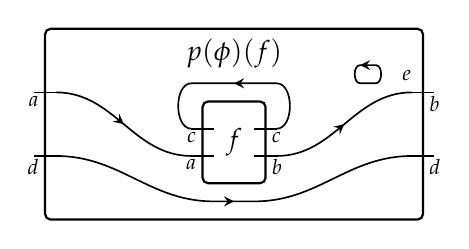
\begin{tikzpicture}[wiring diagram, bby=1.4ex, baseline=(current bounding box.center)]
      \node[bb port sep=1.5, bb={2}{2}] (domain) {$f$};
      \node[bb={2}{2}, fit={(domain) ($(domain.north)+(0,3)$) ($(domain.south)-(0,1)$)}, bb name=$p(\phi)(f)$] (codomain) {};
      \draw[ar] (codomain_in1') to (domain_in2);
      \draw[ar] (domain_out2) to (codomain_out1');
      \draw[ar] let \p1=(domain.north east), \p2=(domain.north west), \n1={\y1+\bby}, \n2=\bbportlen in
          (domain_out1) to[in=0] (\x1+\n2,\n1) -- (\x2-\n2,\n1) to[out=180] (domain_in1);  %trace on c
      \draw[ar] let \p1=(domain.south west), \p2=(domain.south east), \n1={\y1-\bby}, \n2=\bbportlen in
          (codomain_in2') to[in=180] (\x1+\n2,\n1) -- (\x2-\n2,\n1) to[out=0] (codomain_out2'); %identity on d
      \draw[ar] let \p1=(domain.north east) in
          (\x1+.7*\bbx,\y1+\bby) to[in=0] (\x1+.7*\bbx,\y1+2*\bby) -- (\x1+.6*\bbx,\y1+2*\bby) to[out=180] (\x1+.6*\bbx,\y1+\bby) -- (\x1+.7*\bbx,\y1+\bby);%loop
      \draw[label] let \p1=(domain.north east) in
          node[below left=of codomain_in1]     {$a$}
          node[below left=of codomain_in2]     {$d$}
          node[below right=of codomain_out1]    {$b$}
          node[below right=of codomain_out2]    {$d$}
          node[above left=.6 and 0 of codomain_out1']  {$e$}
          node[below left=of domain_in1]     {$c$}
          node[below left=of domain_in2]     {$a$}
          node[below right=of domain_out2]    {$b$}
          node[below right=of domain_out1]   {$c$};
   \end{tikzpicture}
   \qquad\qquad
   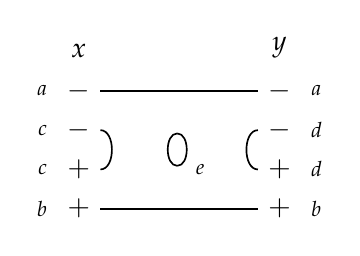
\begin{tikzpicture}[x=1cm,y=1ex,node distance=1 and 1,semithick,every label quotes/.style={font=\everymath\expandafter{\the\everymath\scriptstyle}},every to/.style={out=0,in=180},baseline=(current bounding box.center)]
      \node ["$a$" left] (x1a) {$-$};
      \node [above=0.25 of x1a] {$x$};
      \node [below=0 of x1a, "$c$" left] (x1b) {$-$};
      \node [below=0 of x1b, "$c$" left] (x2a) {$+$};
      \node [below=0 of x2a, "$b$" left] (x2b) {$+$};
      \node [right=2 of x1a, "$a$" right] (y1a) {$-$};
      \node [above=0.25 of y1a] {$y$};
      \node [below=0 of y1a, "$d$" right] (y1b) {$-$};
      \node [below=0 of y1b, "$d$" right] (y2a) {$+$};
      \node [below=0 of y2a, "$b$" right] (y2b) {$+$};
      \node [right=1.45 of x2a, "$e$" left] {};
      \draw (x1a) to (y1a);
      \draw (x1b) to[in=0] (x2a);
      \draw (x2b) to (y2b);
      \draw (y1b) to[in=180,out=180] (y2a);
      \draw ($(x1b)+(1.25,-2.75)$) to[in=0] ($(x1b)+(1.25,-0.25)$);
      \draw ($(x1b)+(1.25,-0.25)$) to[in=180,out=180] ($(x1b)+(1.25,-2.75)$);
   \end{tikzpicture}
\end{equation}
with the above notation, for $f\in p(x)$ we can follow the string diagram (left of (\ref{eq:cob_and_trace_pic})) and define
\begin{equation}\label{eq:cob algebra formula}
   p(\phi)(f)\coloneqq\tr_{a,b}^c(f)\otimes d\otimes\tr^e_{i,i}(\id_e).
\end{equation}


\section{applications of the operadic perspective}

the operadic perspective on traced categories may be useful in concrete applications, such as for
modeling nested process diagrams. it may also be useful in pure mathematics, because the operad $\cob$,
which indexes traced categories, can be easily modified to model a variety of other doctrines.
these two applications will be discussed in more detail in
sections~\ref{subsec:modular}~and~\ref{subsec:math_application} respectively.

\subsection{modular design}\label{subsec:modular}

when designing or investigating a complex system, it is often useful to think in terms of
interacting subsystems, put together to make a larger whole. in manufacturing, this is often called
\emph{modular design}. each object in $\cob$ represents an interface, or \emph{module}, with a
fixed number and type of inputs and outputs. the morphisms in $\cob$ correspond to strategies by
which these interfaces can be wired together into a process, which itself has an interface (the outer box).

an algebra $p\colon\cob\to\set$ provides semantics for these interfaces (\cite{rupelspivak},\cite{vagnerspivaklerman}). for each interface $x$, the set
$p(x)$ represents the set of possible ``fillers'' for it. for example, one might imagine that
each interface $x$ can be filled by any state machine having that interface; in this case $p(x)$ would be
the set of such state machines. for a morphism $\varphi\colon x_1,\ldots,x_n\to y$, the function
$p(\varphi)$ tells us how to construct a filler of interface $y$, given fillers on each $x_i$.
composition of cobordisms are drawn as nested diagrams:
\begin{equation*}
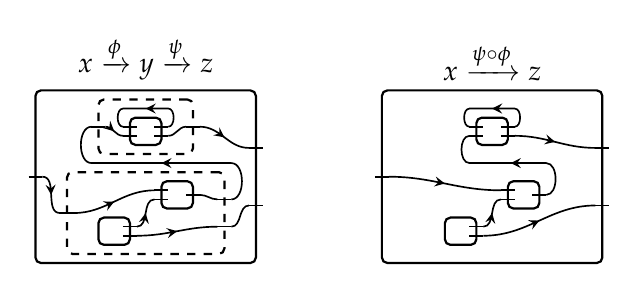
\begin{tikzpicture}[wiring diagram, bb small]
   \node[bb={2}{2}] (x1) {};
   \node[bb={1}{1}, fit={(x1) ($(x1.north)+(0,1)$)}, dashed] (y1) {};
   \node[bb={2}{1}, below right=4 and 0 of x1] (x2) {};
   \node[bb={0}{2},below left=of x2] (x3) {};
   \node[bb={1}{2}, fit=(x2) (x3), dashed] (y2) {};
   \node[bb={1}{2}, fit=(y1) (y2)] (z) {};
   \draw[ar] (z_in1') to (y2_in1);
   \draw[ar] (y2_in1') to (x2_in1);
   \draw[ar] (x3_out1) to (x2_in2);
   \draw[ar] (x3_out2) to (y2_out2');
   \draw (y2_out2) to (z_out2');
   \draw[ar] (y1_in1') to (x1_in2);
   \draw (x1_out2) to (y1_out1');
   \draw[ar] (y1_out1) to (z_out1');
   \draw (x2_out1) to (y2_out1');
   \draw[ar] let \p1=(y2.north east), \p2=(y1.south west), \n1={\y1+\bby}, \n2=\bbportlen in
      (y2_out1) to[in=0] (\x1+\n2,\n1) -- (\x2-\n2,\n1) to[out=180] (y1_in1);
   \draw[ar] let \p1=(x1.north east), \p2=(x1.north west), \n1={\y1+\bby}, \n2=\bbportlen in
      (x1_out1) to[in=0] (\x1+\n2,\n1) -- (\x2-\n2,\n1) to[out=180] (x1_in1);
   \node[anchor=south] at (z.north) {$x\xrightarrow{\phi}y\xrightarrow{\psi}z$};

   \node[bb={2}{2}, right=10 of x1] (x1') {};
   \node[bb={2}{1}, below right=4 and 0 of x1'] (x2') {};
   \node[bb={0}{2},below left=of x2'] (x3') {};
   \node[bb={1}{2}, fit={($(x1'.north)+(0,1)$) (x2') (x3')}, inner xsep=2*\bbx, inner ysep=2*\bby] (z') {};
   \draw[ar] (x3'_out1) to (x2'_in2);
   \draw[ar] (z'_in1') to (x2'_in1);
   \draw[ar] (x1'_out2) to (z'_out1');
   \draw[ar] (x3'_out2) to (z'_out2');
   \draw[ar] let \p1=(x2'.north east), \p2=(x1'.south west), \n1={\y1+2*\bby}, \n2=\bbportlen in
      (x2'_out1) to[in=0] (\x1+\n2,\n1) -- (\x2-\n2,\n1) to[out=180] (x1'_in2);
   \draw[ar] let \p1=(x1'.north east), \p2=(x1'.north west), \n1={\y1+\bby}, \n2=\bbportlen in
      (x1'_out1) to[in=0] (\x1+\n2,\n1) -- (\x2-\n2,\n1) to[out=180] (x1'_in1);
   \node[anchor=south] at (z'.north) {$x\xrightarrow{\psi\circ\phi}z$};
\end{tikzpicture}
\end{equation*}

in our model for modular design, any way to chunk the small boxes inside the big one will yield the
same result. this is a reflection of the functoriality of $p\colon\cob\to\set$, which says that
commutative diagrams in $\cob$ are sent to commutative diagrams of sets. nested structures, given
by composition of such morphisms, may be useful for the kind of chunking that humans use to
understand complex systems~\cite{miller}.

\subsection{mathematical application: varying the operad}\label{subsec:math_application}

formalizing modular design using operads, as in~\cite{spivak},~\cite{rupelspivak},
and~\cite{vagnerspivaklerman} was the original motivation for the present paper, as the drawings had
strong similarities to those found in traced categories. however, it should be noted that none of
these papers actually uses $\cob$ as the indexing category for their algebras, and hence none are
actually directly related to traced categories. in fact, they use three different operads, of
varying degrees of similarity to $\cob$. for example, there is an orthogonal factorization system on
$\cob$ \cite{abadi}, for which morphisms in the left class $\cat{l}$ include no closed loops, and
the operad of interest in~\cite{vagnerspivaklerman} is $\cat{l}$.

if one wished to make minor modifications in the axioms of traced categories to create some new sort
of category $\ncat{tr'cat}$, one may proceed by imagining the string diagrams that make sense in
$\ncat{tr'cat}$. for example, one may want to consider cartesian traced categories, in which wires
can split or terminate abruptly. or one might want to allow splitting but not allow abrupt
termination.
\begin{equation*}
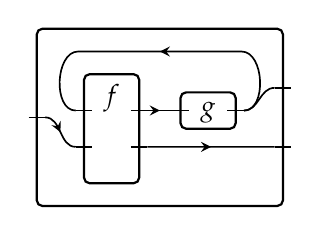
\begin{tikzpicture}[wiring diagram,bb min width =.7cm, bb port sep =1, bbx=.6cm,bb port length=3pt]
   \node[bb port sep=1.6, bb={2}{2}, bb name=$f$] (x1) {};
   \node[bb port sep=.8,bb={1}{1}, right=.7 of x1_out1, bb name=$g$] (x2) {};
   \node[bb={1}{2}, fit={(x1) (x2) ($(x1.north)+(0,1)$)}] (y) {};
   \draw[ar] (y_in1') to (x1_in2);
   \draw[ar,pos=.8] (x1_out1) to (x2_in1);
   \draw (x2_out1) to (y_out1');
   \draw[ar] (x1_out2) to (y_out2');
   \draw[ar] let \p1=(x2.north east), \p2=(x1.north west), \n1={\y2+\bby}, \n2=\bbportlen in
      (x2_out1) to[in=0] (\x1+.7*\n2,\n1) -- (\x2-.7*\n2,\n1) to[out=180] (x1_in1);
\end{tikzpicture}
\end{equation*}
we can accommodate any such modification of string diagrams for $\ncat{tr'cat}$ by modifying the
indexing operad $\cob$ to some $\cob'$. using $\cat{l}$ for dynamical systems in
\cite{vagnerspivaklerman} is an example of this. as another, suppose that, as above, we want string
diagrams in which wires can split but not terminate. noting that an oriented cobordism $\varphi$
includes the data of a function
\begin{equation*}
   \varphi\colon\inp{x}\sqcup\outp{y}\to\outp{x}\sqcup\inp{y},
\end{equation*}
which is both injective and surjective, we can obtain the desired indexing operad $\cob'$ by
requiring surjectivity but not injectivity in $\varphi$.


\section{plan of the paper}

in section~\ref{chap:traced_categories} we review monoidal, traced, and compact categories, as well
as the notion of orthogonal factorization systems. in section~\ref{chap:background_equipments} we
review equipments (also known as framed bicategories) \cite{shulman}, and exact equipments
\cite{schultz2015}. in section~\ref{sec:internal_presheaves} we record the definition of
copresheaves internal to an equipment, which we need to properly express our main theorems. we
finally introduce the equipments of primary interest, $\dmonprof, \dtrprof$, and $\dcompprof$ in
section~\ref{chap:equipments_monoidal_profunctors}. we prove that they are exact in
section~\ref{sec:exactness_proofs} and, in section~\ref{sec:special_compprof}, prove the special
properties about $\dcompprof$ which are at the core of our results. indeed one might view the rest
of the paper as a formal wrapper for the results in that section. in
section~\ref{sec:monoids_on_free} we deal with object-freeness, which we need for
\ref{thm:theorema}. we deduce it as well as \ref{thm:theoremb} in section~\ref{sec:deducing}.

\section*{acknowledgments}

thanks go to steve awodey and ed morehouse for suggesting we formally connect the operad-algebra
picture in \cite{rupelspivak} to string diagrams in traced categories. we also thank mike shulman
and justin hilburn for many useful conversations.

\chapter{categorical preliminaries}\label{chap:traced_categories}

in this section we remind the reader of some categorical preliminaries. basic definitions and facts
about monoidal, traced, and compact categories, lax and strong functors, and the int construction
are given in sections~\ref{sec:prelim_monoidal}~through~\ref{sec:compact_and_int}. the fact that the
free compact category on a set has an algebraic description in terms signed sets and bijections, and
the fact that it has a geometric description in terms of 1-dimensional oriented cobordisms is
recalled in section~\ref{sec:free_and_geometry}.

\section{monoidal categories}\label{sec:prelim_monoidal}

let $\cat{c}$ and $\cat{d}$ be monoidal categories. recall that a functor
$f\colon\cat{c}\to\cat{d}$ is called \emph{lax monoidal} if it is equipped with a morphism
\[
\begin{tikzcd}
   i_d \rar{\mu} & f(i_c)
\end{tikzcd}
\]
and a natural transformation
\[
\begin{tikzcd}
   f(x) \otimes_d f(y) \rar{\mu_{x,y}} & f(x\otimes_c y)
\end{tikzcd}
\]
such that for all $x,y,z\in\cat{c}$, the diagram (suppressing associators)
\[
\begin{tikzcd}
   f(x)\otimes f(y) \otimes f(z)
      \rar{f(x)\otimes\mu}
      \dar[swap]{\mu\otimes f(z)}
   & f(x)\otimes f(y\otimes z)
      \dar{\mu} \\
   f(x\otimes y)\otimes f(z)
      \rar[swap]{\mu}
   & f(x\otimes y\otimes z)
\end{tikzcd}
\]
commutes, and for all $x\in\cat{c}$ the two diagrams
\[
\begin{tikzcd}
   i_d\otimes f(x)
      \dar[swap]{\mu\otimes f(x)}
   & f(x)
      \lar[swap]{\lambda_{f(x)}}
      \dar{f(\lambda_x)} \\
   f(i_c)\otimes f(x)
      \rar[swap]{\mu}
   & f(i_c\otimes x)
\end{tikzcd}
\qquad
\begin{tikzcd}
   f(x) \otimes i_d
      \dar[swap]{f(x)\otimes\mu}
   & f(x)
      \lar[swap]{\rho_{f(x)}}
      \dar{f(\rho_x)} \\
   f(x)\otimes f(i_c)
      \rar[swap]{\mu}
   & f(x\otimes i_c)
\end{tikzcd}
\]
commute, where $\lambda$ and $\rho$ are unitors.
if all $\mu$'s are isomorphisms, then $f$ is \emph{strong}.

if $\cat{c}$ and $\cat{d}$ are symmetric monoidal, then $f$ is a \emph{lax symmetric monoidal
functor} if it is lax monoidal, and commutes with the symmetries, in the sense that the diagram
\[
\begin{tikzcd}
   f(x)\otimes f(y)
      \rar{\sigma}
      \dar[swap]{\mu}
   & f(y)\otimes f(x)
      \dar{\mu} \\
   f(x\otimes y)
      \rar[swap]{f(\sigma)}
   & f(y\otimes x)
\end{tikzcd}
\]
commutes.

if $f$ and $g$ are lax monoidal functors (possibly symmetric), then a natural transformation
$\alpha\colon f\to g$ is called a \emph{monoidal transformation} if the diagrams
\[
\begin{tikzcd}
   f(x)\otimes f(y)
      \rar{\alpha_x\otimes\alpha_y}
      \dar[swap]{\mu}
   & g(x)\otimes g(y)
      \dar{\mu} \\
   f(x\otimes y)
      \rar[swap]{\alpha_{x\otimes y}}
   & g(x\otimes y)
\end{tikzcd}
\qquad
\begin{tikzcd}[column sep=tiny]
   {} & i_d \dlar[swap]{\mu} \drar{\mu} & \\
   f(i_c) \ar{rr}[swap]{\alpha_i} && g(i_c)
\end{tikzcd}
\]
commute.

let $\mmoncat$ denote the 2-category of symmetric monoidal categories, strong monoidal functors, and
monoidal transformations, and let $\moncat$ denote the underlying 1-category. let
$\lax(\cat{c},\cat{d})$ denote the category of lax monoidal functors and monoidal transformations
from $\cat{c}$ to $\cat{d}$.

\begin{warning}\label{warn:symmetric}
   for the rest of this article, whenever we discuss monoidal categories, we will mean symmetric
   monoidal categories. for example, see the definition of $\mmoncat$ above.
\end{warning}

\section{traced categories}\label{sec:intuition_for_traced}

a \emph{trace structure} on a (symmetric) monoidal category $\cat{m}$ is a collection of functions
\begin{equation}\label{dia:trace function}
   \tr^u_{x,y}\colon\hom_{\cat{m}}(u\otimes x,u\otimes y)\to\hom_{\cat{m}}(x,y)
\end{equation}
for $u,x,y\in\ob(\cat{m})$ satisfying several, say six, equational axioms. when traced categories
are defined, e.g., in \cite{joyalstreetverity}, one often sees the trace functions, as well as each
of the axioms, accompanied by a picture. for example, (\ref{dia:trace function}) applied to an
arbitrary morphism $f\colon u\otimes x\to u\otimes y$ might be accompanied by this picture:
\begin{equation*}
   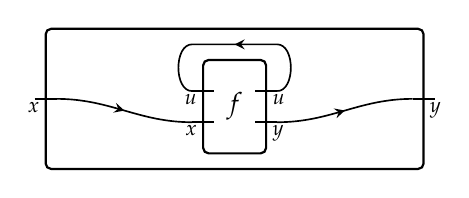
\begin{tikzpicture}[wiring diagram,bby=1.2ex]
      \node[bb={2}{2}] (domain) {$f$};
      \node[bb={1}{1}, fit={(domain) ($(domain.north)+(0,1)$)}] (codomain) {};
      \draw[ar] (codomain_in1') to (domain_in2);
      \draw[ar] (domain_out2) to (codomain_out1');
      \draw[ar] let \p1=(domain.north east), \p2=(domain.north west), \n1={\y1+\bby}, \n2=\bbportlen in
         (domain_out1) to[in=0] (\x1+\n2,\n1) -- (\x2-\n2,\n1) to[out=180] (domain_in1);
      \draw[label]
          node[below left=of codomain_in1]     {$x$}
          node[below right=of codomain_out1]    {$y$}
          node[below left=of domain_in1]     {$u$}
          node[below left=of domain_in2]     {$x$}
          node[below right=of domain_out2]    {$y$}
          node[below right=of domain_out1]   {$u$};
   \end{tikzpicture}
\end{equation*}
this can be recognized as a cobordism between oriented 0-manifolds, as we discussed in
section~\ref{subsec:wds_and_cob}. each of the six axioms is vacuous from this perspective, in
the sense that both sides of the equation correspond to the same cobordism (up to diffeomorphism). for example, here are
the axioms of \emph{dinaturality} and \emph{superposition}:
\begin{itemize}
   \item for every $f\colon u\otimes x\to v\otimes y$ and $g:v\to u$ we have
      \[
         \tr^u_{x,y}\big[\big(g\otimes y\big)\circ f\big]=\tr^v_{x,y}\big[f\circ\big(g\otimes x\big)\big];
      \]
      \[\tikzset{bbx=1cm}
         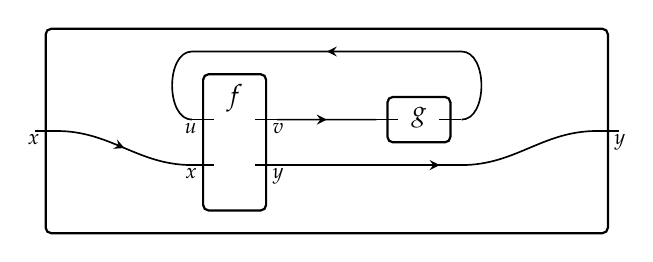
\begin{tikzpicture}[wiring diagram,baseline=(current bounding box.center)]
            \node[bb={2}{2}, bb name=$f$] (x1) {};
            \node[bb port sep=1,bb={1}{1}, right=.7 of x1_out1, bb name=$g$] (x2) {};
            \node[bb={1}{1}, fit={(x1) (x2) ($(x1.north)+(0,1)$)}] (y) {};
            \draw[ar] (y_in1') to (x1_in2);
            \draw[ar,pos=.8] (x1_out1) to (x2_in1);
            \draw[ar] let \p1=(x2.south east), \n1={\y1-\bby}, \n2=\bbportlen in
                (x1_out2) -- (\x1+\n2,\n1) to (y_out1');
            \draw[ar] let \p1=(x2.north east), \p2=(x1.north west), \n1={\y2+\bby}, \n2=\bbportlen in
                  (x2_out1) to[in=0] (\x1+\n2,\n1) -- (\x2-\n2,\n1) to[out=180] (x1_in1);
            \draw[label]
                node[below left=of y_in1]     {$x$}
                node[below right=of y_out1]    {$y$}
                node[below left=of x1_in1]     {$u$}
                node[below left=of x1_in2]     {$x$}
                node[below right=of x1_out2]    {$y$}
                node[below right=of x1_out1]   {$v$};
         \end{tikzpicture}
         \quad=\quad
         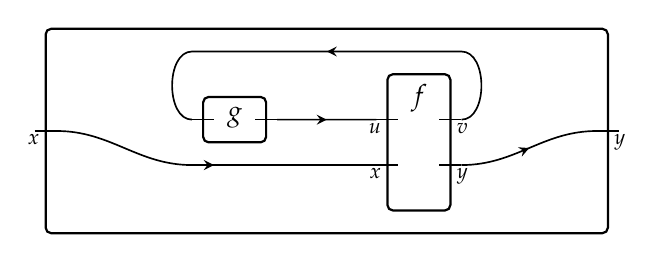
\begin{tikzpicture}[wiring diagram,baseline=(current bounding box.center)]
            \node[bb={2}{2}, bb name=$f$] (x1) {};
            \node[bb port sep=1,bb={1}{1}, left=.7 of x1_in1, bb name=$g$] (x2) {};
            \node[bb={1}{1}, fit={(x1) (x2) ($(x1.north)+(0,1)$)}] (y) {};
            \draw[ar] let \p1=(x2.south west), \n1={\y1-\bby}, \n2=\bbportlen in
                (y_in1') to (\x1-\n2,\n1) -- (x1_in2);
            \draw[ar] (x2_out1) to (x1_in1);
            \draw[ar] (x1_out2) to (y_out1');
            \draw[ar] let \p1=(x1.north east), \p2=(x2.north west), \n1={\y1+\bby}, \n2=\bbportlen in
                  (x1_out1) to[in=0] (\x1+\n2,\n1) -- (\x2-\n2,\n1) to[out=180] (x2_in1);
            \draw[label]
                node[below left=of y_in1]     {$x$}
                node[below right=of y_out1]    {$y$}
                node[below left=of x1_in1]     {$u$}
                node[below left=of x1_in2]     {$x$}
                node[below right=of x1_out2]    {$y$}
                node[below right=of x1_out1]   {$v$};
         \end{tikzpicture}
         \]
   \item for every $f\colon u\otimes x\to u\otimes y$ and $g\colon w\to z$ we have
      \[
         \tr^u_{x,y}\big[f\big]\otimes g=\tr^u_{x\otimes w,y\otimes z}\big[f\otimes g\big];
      \]
      \[\tikzset{bbx=.8cm,bb port sep=1.5}
      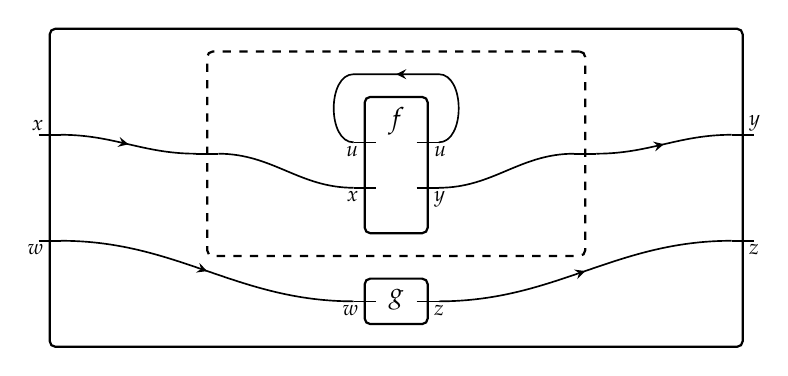
\begin{tikzpicture}[wiring diagram,baseline=(current bounding box.center)]
         \node[bb={2}{2}, bb name=$f$] (x1) {};
         \node[bb port sep=1,bb={1}{1}, below=2 of x1, bb name=$g$] (x2) {};
         \node[bb={1}{1}, fit={(x1) ($(x1.north)+(0,1)$)}, dashed] (z) {};
         \node[bb={2}{2}, fit={(z) (x2)}] (y) {};
         \draw[ar] (y_in1') to (z_in1);
         \draw (z_in1') to (x1_in2);
         \draw[ar] (y_in2') to (x2_in1);
         \draw (x1_out2) to (z_out1');
         \draw[ar] (z_out1) to (y_out1');
         \draw[ar] (x2_out1) to (y_out2');
         \draw[ar] let \p1=(x1.north east), \p2=(x2.north west), \n1={\y1+\bby}, \n2=\bbportlen in
             (x1_out1) to[in=0] (\x1+\n2,\n1) -- (\x2-\n2,\n1) to[out=180] (x1_in1);
         \draw[label]
             node[above left=of y_in1] {$x$}
             node[below left=of y_in2] {$w$}
             node[above right=of y_out1] {$y$}
             node[below right=of y_out2] {$z$}
             node[below left=of x1_in1] {$u$}
             node[below left=of x1_in2] {$x$}
             node[below right=of x1_out2] {$y$}
             node[below right=of x1_out1] {$u$}
             node[below left=of x2_in1] {$w$}
             node[below right=of x2_out1] {$z$};
      \end{tikzpicture}
      \quad=\quad
      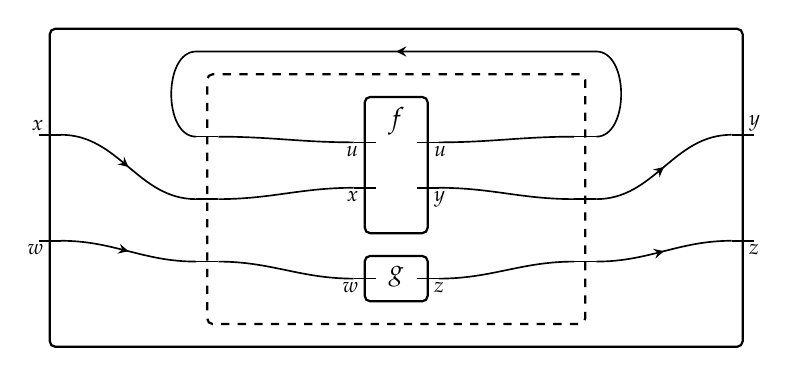
\begin{tikzpicture}[wiring diagram,baseline=(current bounding box.center)]
         \node[bb={2}{2}, bb name=$f$] (x1) {};
         \node[bb port sep=1,bb={1}{1}, below=of x1, bb name=$g$] (x2) {};
         \node[bb={3}{3}, fit={(x1) (x2)}, dashed] (z) {};
         \node[bb={2}{2}, fit={(z) ($(z.north)+(0,1)$)}] (y) {};
         \draw[ar] (y_in1') to (z_in2);
         \draw (z_in2') to (x1_in2);
         \draw[ar] (y_in2') to (z_in3);
         \draw (z_in3') to (x2_in1);
         \draw (x1_out2) to (z_out2');
         \draw[ar] (z_out2) to (y_out1');
         \draw (x2_out1) to (z_out3');
         \draw[ar] (z_out3) to (y_out2');
         \draw (z_in1') to (x1_in1);
         \draw (x1_out1) to (z_out1');
         \draw[ar] let \p1=(z.north east), \p2=(z.north west), \n1={\y1+\bby}, \n2=\bbportlen in
             (z_out1) to[in=0] (\x1+\n2,\n1) -- (\x2-\n2,\n1) to[out=180] (z_in1);
         \draw[label]
             node[above left=of y_in1] {$x$}
             node[below left=of y_in2] {$w$}
             node[above right=of y_out1] {$y$}
             node[below right=of y_out2] {$z$}
             node[below left=of x1_in1] {$u$}
             node[below left=of x1_in2] {$x$}
             node[below right=of x1_out2] {$y$}
             node[below right=of x1_out1] {$u$}
             node[below left=of x2_in1] {$w$}
             node[below right=of x2_out1] {$z$};
      \end{tikzpicture}
      \]
\end{itemize}

the definition of traced categories and traced functors can be found in~\cite{joyalstreetverity}. however, those authors define the 2-morphisms between traced functors to be monoidal transformations, whereas this choice does not behave appropriately with their $\int$ construction (for example $\int$ would not be 2-functorial). a correction was made in \cite{hk}, where it was shown that the appropriate 2-morphisms between traced functors are natural \emph{isomorphisms}. we denote by $\ttrcat$ the corrected 2-category of traced categories (where 2-cells are invertible), and we denote its underlying 1-category by $\trcat$.

%\subsection{the categories $\prop$ and $\trprop$ of props and traced props}\label{sec:defining props}
%\todo{do we want to use this section anywhere?}
%
%one can think of a prop as a symmetric monoidal category whose objects are free on a fixed set of \emph{labels}
%(also known as its set of colors). functors between props need to descend to a function between
%label sets. we define a traced prop to be a traced category whose underlying symmetric monoidal
%category has the structure of a prop. thus we have defined the 1-categories $\prop$ and $\trprop$;
%we summarize our definitions by the pullback diagram of categories
%\[
%\begin{tikzcd}
%   \trprop\ar[r]\ar[d]\arrow[dr, phantom, "\lrcorner", very near start]&\trcat\ar[d]\\
%   \prop\ar[r]\ar[d,"\tn{labels}"']\arrow[dr, phantom, "\lrcorner", very near start]&\moncat\ar[d,"\ob"]\\
%   \set\ar[r,"\tm"']&\set
%\end{tikzcd}
%\]
%where $\tm\colon\set\to\set$ is the free monoid monad. this definition of $\prop$
%agrees with that in~\cite{hackneyrobertson}.\todo{check this.}
%

\section{compact categories and the int construction}\label{sec:compact_and_int}

we will denote by $\ccompcat$ the full sub-2-category of $\mmoncat$ spanned by the compact symmetric
monoidal categories (or just compact categories for short).  recall that a compact category is a
symmetric monoidal category $(\cat{c},\otimes,i)$ with the property that for every object
$x\in\cat{c}$ there exists an object $x^*$ and morphisms $\eta_x\colon i\to x^*\otimes x$ and
$\epsilon_x\colon x\otimes x^*\to i$ such that the following diagrams commute:
\begin{equation*}
   \begin{tikzcd}[column sep=small]
      x\arrow[r,"\id_x"]\arrow[d,"\cong"'] & x \\
      x\otimes i\arrow[d,"x\otimes\eta_x"'] & i\otimes x\arrow[u,"\cong"'] \\
      x\otimes(x^*\otimes x)\arrow[r,"\cong"'] & (x\otimes x^*)\otimes x\arrow[u,"\epsilon_x\otimes x"']
   \end{tikzcd}
   \hspace{.6in}
   \begin{tikzcd}[column sep=small]
      x^*\arrow[r,"\id_{x^*}"]\arrow[d,"\cong"'] & x^*\\
      i\otimes x^*\arrow[d,"\eta_x\otimes x^*"'] & x^*\otimes i\arrow[u,"\cong"'] \\
      (x^*\otimes x)\otimes x^*\arrow[r,"\cong"'] & x^*\otimes (x\otimes x^*)\arrow[u,"x^*\otimes\epsilon_x"']
   \end{tikzcd}
\end{equation*}

every compact category $\cat{c}$ has a canonical trace structure, defined on a morphism $f\colon
u\otimes x\to u\otimes y$ morally (up to symmetries and identities) to be $\epsilon_u\circ f\circ \eta_u$. more precisely, if
$\sigma_{a,b}$ is the symmetry isomorphism, one defines
\begin{equation*}
   \tr^u_{x,y}[f]\coloneqq(\epsilon_u\otimes y)\circ (\sigma_{u^*,u}\otimes y)\circ (u^*\otimes f)\circ (\eta_u\otimes x)
\end{equation*}
thus we have a functor $\uct\colon\ccompcat\to\ttrcat$. it is shown in~\cite{joyalstreetverity}~and~\cite{hk} that
this functor is the right half of a 2-adjunction
\begin{equation}\label{dia:traced_compact_adjunction}
\begin{tikzcd}
   \ttrcat\arrow[r,shift left=.5ex, "\int"]&\ccompcat\arrow[l,shift left=.5ex,"\uct"]
\end{tikzcd}
\end{equation}
the left half of which we now describe on the level of objects $\cat{m}\in\ttrcat$.

for a traced category $\cat{m}$, let $\widetilde{\cat{m}}$ denote the category with
objects given by pairs $(\inp{x},\outp{x})$ where $\inp{x},\outp{x}\in(\cat{m})$ and morphisms
given by
\[
   \hom_{\widetilde{\cat{m}}}\big((\inp{x},\outp{x}),(\inp{y},\outp{y})\big)=\hom_{\cat{m}}(\inp{x}\otimes \outp{y},\outp{x}\otimes \inp{y}).
\]
for morphisms $\phi:(\inp{x},\outp{x})\to(\inp{y},\outp{y})$ and $\psi:(\inp{y},\outp{y})\to(\inp{z},\outp{z})$ in $\widetilde{\cat{m}}$ we define their composition to be
\[
   \psi\circ\phi\coloneqq\tr^{\outp{y}}_{\inp{x}\otimes \outp{z},\outp{x}\otimes \inp{z}}\big[\big(\sigma_{\outp{x},\outp{y}}\otimes \inp{z}\big)\circ\big(\outp{x}\otimes\psi\big)\circ\big(\phi\otimes \outp{z}\big)\circ\big(\sigma_{\outp{y},\inp{x}}\otimes \outp{z}\big)\big].
\]
it is shown in~\cite{joyalstreetverity} that $\int(\cat{m})\coloneqq\widetilde{\cat{m}}$ is a compact category whose tensor is given by
\[
   (\inp{x},\outp{x})\odot(\inp{y},\outp{y})\coloneqq(\inp{x}\otimes \inp{y},\outp{x}\otimes \outp{y})
\]
with unit object $\tilde i\coloneqq(i,i)$ and duality ${(\inp{x},\outp{x})}^\vee\coloneqq(\outp{x},\inp{x})$.

\begin{lemma}\label{lemma:fully_faithful_and_trace}
the following facts hold for any traced category $\cat{c}$:
\begin{compactenum}[\quad i.]
   \item the unit $\cat{c}\to\int(\cat{c})$ is fully faithful.
   \item if $\cat{d}$ is a category and $f\colon\cat{d}\to\cat{c}$ a fully faithful symmetric
      monoidal functor, then $\cat{d}$ has a unique trace for which $f$ is a traced functor.
   \item if $\cat{c}$ is compact then the unit $\cat{c}\to{\raisebox{-1ex}{$\equiv$}}\int(\cat{c})$ is an equivalence.
   \item suppose that $\cat{c'}$ is a traced category and that $f\colon \cat{c}\to \cat{c}'$ is a
      traced functor. then $f$ is bijective-on-objects (resp. fully faithful) if and only if
      $\int(f)$ is.
\end{compactenum}
\end{lemma}
\begin{proof}
   these are all shown in, or trivially derived from,~\cite{joyalstreetverity}.
\end{proof}

\section{free traced and compact categories, and geometry}\label{sec:free_and_geometry}

there are free/forgetful adjunctions
\begin{align*}
   \fm\colon\set &\leftrightarrows\moncat:\!\um \\
   \ft\colon\set &\leftrightarrows\trcat:\!\ut \\
   \fc\colon\set &\leftrightarrows\compcat:\!\uc
\end{align*}
we will write $\tm, \tt$, and $\tc$ for the respective monads induced on $\set$. note that $\tm$ is
isomorphic to the free monoid monad, while $\tc$ is isomorphic to the free monoid-with-involution
monad.%
\footnote{
   note that $u_m$ is not the free-\emph{commutative}-monoid monad, even though the objects of
   $\moncat$ are \emph{symmetric} monoidal categories, because the symmetries are encoded in natural
   isomorphisms, not equalities.
}
we will denote by $\frmoncat$ and $\frcompcat$ the full subcategories of $\moncat$ and $\compcat$
respectively, spanned by objects which are free on a set. as always, these categories are isomorphic
to the kleisli categories of the monads:
\begin{align}\label{dia:tmvsfrmoncat}
\frmoncat&\iso\set_{\tm}
\\\nonumber
\frcompcat&\iso\set_{\tc}.
\end{align}

the forgetful functors between the categories of structured monoidal categories commute with the
underlying set functors, i.e.~the following diagram commutes:
%\begin{equation*}
%	\begin{tikzcd}[column sep=large]
%	\compcat\ar[r,"\uct"]\ar[rd,"\uc"']\ar[rr,bend left,"\ucm"]&\trcat\ar[r,"\utm"]\ar[d,"\ut"]&\moncat\ar[dl,"\um"]\\
%	&\set
%	\end{tikzcd}
%\end{equation*}

\begin{equation}\label{eqn:tetrahedron}
   \begin{tikzcd}
      & \trcat \ar[dr,"\utm"] \ar[dd,"\ut" near start] & \\
      \compcat \ar[rr,crossing over,"\ucm"' near start] \ar[dr,"\uc"'] \ar[ru,"\uct"]
         && \moncat \ar[dl,"\um"] \\
      & \set &
   \end{tikzcd}
\end{equation}
because the functor $\ucm\colon\compcat\to\moncat$ commutes with the right adjoints of the
adjunctions to $\set$, i.e., $\um\ucm=\uc$, it induces a monad morphism $\alpha\colon\tc\to\tm$ (a natural transformation
$\alpha\colon\tm\to\tc$ compatible with the units and multipications), given by the composition of
the natural transformations
%\begin{equation*}
%   \begin{tikzcd}[column sep=large,row sep=0ex]
%      \tm=\um\fm \ar[r,"\um\fm\eta_c"]
%         & \um\fm\uc\fc = \um\fm\um\ucm\fc \\
%      \um\fm\um\ucm\fc \ar[r,"\um\epsilon_m\ucm\fc"']
%         & \um\ucm\fc = \uc\fc = \tc
%   \end{tikzcd}
%\end{equation*}
\begin{equation*}
	\begin{tikzcd}[column sep=2cm]
		\tm\ar[r,equal]\ar[d,dashed,"\alpha"']&\um\fm\ar[r,"\um\fm\eta_c"]&\um\fm\uc\fc\ar[d,equal]\\
		\tc&\um\ucm\fc\ar[l,equal]&\um\fm\um\ucm\fc\ar[l,"\um\epsilon_m\ucm\fc"]
	\end{tikzcd}
\end{equation*}
the component $\alpha_{\labset}$ of this transformation is simply the evident inclusion of the free
monoid on a set $\labset$ into the free monoid-with-involution on $\labset$. in this way, $\ucm$
induces a functor between the kleisli categories in the other direction:
\begin{equation}\label{eqn:fmc}
   \fmc\colon\frmoncat\to\frcompcat
\end{equation}

%\begin{proposition}\label{prop:free traced and compact}
%   let $\cat{c}$ be a category.
%   the free traced category on $\cat{c}$ is...
%   the free compact category on $\cat{c}$ is $\int(...)$.\todo{fill this in}
%\end{proposition}
%\begin{proof}
%   kelly, laplaza ``coherence for compact closed categories'' gives a combinatorial description of
%   the free compact category on one object.
%
%   see abramsky.
%\end{proof}

\subsection{$\lcob{\labset}$ is the free compact category on $\labset$}

to connect the geometry (string diagrams) with the algebra (free compact categories), we recall the
following folklore theorem.

\begin{theorem}
the free compact category on one generator is equivalent to $\cob$, the category of oriented
1-dimensional cobordisms.
\end{theorem}

see \cite[theorem 3.6]{freydyetter} for a proof of the non-symmetric version, \cite{kock} and
\cite{baezdolan} for the 2-dimensional version with brief comments on the 1-dimensional version. see
also \cite{kellylaplaza} and \cite{abramsky2} for combinatorial descriptions of $\cob$ as the free
compact category functor.  because the free functor is a left adjoint, hence preserves colimits, we
have the following corollary.

\begin{corollary}\label{cor:free_compact_is_cob}
   for any set $\labset$, the free compact category on $\labset$ is equivalent to $\lcob{o}$, the
   category of oriented $\labset$-labeled 1-cobordisms.
\end{corollary}

%   joachim kock proves that 2-cob is the free compact category on a frobenius algebra object, and
%   the proof can be adapted.

\subsection{set-theoretic description of $\cob$}

here we give a brief description of the category $\cob$, for the reader's convenience. the objects are signed sets, $x=(\inp{x},\outp{x})$. a morphism $x\to y$ can be identified with a set $c$ and four injections (left-hand side of \eqref{eqn:describing_cob}):
\begin{equation}\label{eqn:describing_cob}
\begin{tikzcd}[row sep=1cm, column sep = 1cm]
	&\inp{x}\ar[d]\\
	\outp{x}\ar[r]&c&\inp{y}\ar[l]\\
	&\outp{y}\ar[u]
\end{tikzcd}
\hspace{.6in}
\begin{tikzcd}[row sep=.5cm, column sep =.5cm]
	&\inp{x}\ar[d]\\
	\outp{x}\ar[r]&c&\inp{y}\ar[l]\ar[d]\\
	&\outp{y}\ar[u]\ar[r]&d&\inp{z}\ar[l]\\
	&&\outp{z}\ar[u]
\end{tikzcd}
\end{equation}
such that the image of the vertical maps $\inp{x}+\outp{y}\to c$ is equal to that of the horizontal maps, $\outp{x}+\inp{y}\to c$. composition is acheived by quotienting the middle square in the right-hand diagram of \eqref{eqn:describing_cob}.

\section{orthogonal factorization systems}

we use orthogonal factorization systems throughout this paper, mainly to deal with the issue of
object-variance, mentioned in section~\ref{subsec:main_results}. background on orthogonal
factorization systems can be found in \cite[chapter 5.5]{borceuxv1}. here we describe the
$\cat{v}$-enriched notion, for two cases, the usual 1-categorical case, where $\cat{v}=\set$, and
the strict 2-categorical case, where $\cat{v}=\cat$.

\begin{definition}\label{def:orthogonal}
   let $\cat{v}$ be either $\set$ or $\cat$, and suppose that $\cat{c}$ is a $\cat{v}$-enriched
   category. an \emph{orthogonal factorization system in $\cat{c}$} consists of two distinguished
   classes of morphisms, $(\cat{l},\cat{r})$, with the following properties:
   \begin{itemize}
      \item each morphism $f\in\cat{c}$ factors as $f=e\circ m$, where $m\in\cat{l}$ and
         $e\in\cat{r}$;
      \item if $m\colon a\to b$ in $\cat{l}$ and $e\colon c\to d$ in $\cat{r}$, then the left-hand
         square below is a pullback in $\cat{v}$:
      \begin{equation}\label{eqn:orthfactsys}
         \begin{tikzcd}
            \cat{c}(b,c)\ar[r]\ar[d]\ar[rd,phantom,"\lrcorner" very near start]&\cat{c}(a,c)\ar[d,"e\circ -"]\\
            \cat{c}(b,d)\ar[r,"-\circ m"']&\cat{c}(a,d)
         \end{tikzcd}
         \hspace{.9in}
         \begin{tikzcd}
            a\ar[r,"\forall"]\ar[d,two heads,"m"']&c\ar[d,hook, "e"]\\
            b\ar[r,"\forall"']\ar[ur,dashed,"\exists!"]&d
         \end{tikzcd}
      \end{equation}
      in particular, for all solid arrow squares, as in the right-hand diagram, there exists a
      unique diagonal filler.
   \end{itemize}
   as shown, we often indicate morphisms in $\cat{l}$ using a two-headed arrow, and morphisms in
   $\cat{r}$ using a hooked arrow.
\end{definition}

if $\ccat{c}$ is a 2-category and $\cat{l}, \cat{r}$ are distinguished classes of morphisms, we say
that $\cat{l}$ is \emph{left pseudo-orthogonal} to $\cat{r}$ if the pullback square (left of
\eqref{eqn:orthfactsys}) is only required to be a pseudo-pullback. this means that for any
pseudo-commuting square (right of \eqref{eqn:orthfactsys}), there exists an essentially unique
pseudo-commuting lift.

\begin{example}\label{ex:ess_surj_pseudo_ff}
   in the 2-category $\ccat$, the class of essentially surjective functors is left pseudo-orthogonal
   to the class of fully faithful functors.
\end{example}

\chapter{background on equipments}\label{chap:background_equipments}

this section introduces equipments, which we use to properly situate traced and compact categories.
this tool will eventually allow us to clarify the relationship between strong monoidal functors
between monoidal categories and lax monoidal functors to $\set$. the former are analogous to
functors between categories, whereas the latter are analogous to profunctors.

\section{profunctors}\label{sec:profunctors}
let $\cat{c}$ and $\cat{d}$ be categories.
recall that a profunctor $m$ from $\cat{c}$ to $\cat{d}$, written
\[
   \begin{tikzcd}
      \cat{c} \ar[r,tick,"m"] & \cat{d},
   \end{tikzcd}
\]
is defined to be a functor $m\colon\op{\cat{c}}\times\cat{d}\to\set$. we can think of a profunctor
as a sort of graded bimodule: for each object $c\in\cat{c}$ and $d\in\cat{d}$ there is a set
$m(c,d)$ of elements in the bimodule, and given an element $m\in m(c,d)$ and morphisms $f\colon
c'\to c$ in $\cat{c}$ and $g\colon d\to d'$ in $\cat{d}$, there are elements $g\cdot m\in m(c,d')$
and $m\cdot f\in f(c',d)$, such that the equations $(g\cdot m)\cdot f=g\cdot(m\cdot f)$,
$g'\cdot(g\cdot m)=(g'\circ g)\cdot m$, and $(m\cdot f)\cdot f'=m\cdot(f\circ f')$ hold whenever
they make sense.

if $f\colon\cat{c}'\to\cat{c}$ and $g\colon\cat{d}'\to\cat{d}$ are functors, and $m$ is a profunctor
as before, then there is a profunctor $m(f,g)$ from $\cat{c}'$ to $\cat{d}'$, defined to be the
composite
\[
\begin{tikzcd}
   \op{\cat{c}'}\times\cat{d}' \ar[r,"\op{f}\times g"]
      &[1.5em] \op{\cat{c}}\times\cat{d} \ar[r,"m"]
      & \set.
\end{tikzcd}
\]
in other words, for any objects $c\in\cat{c}'$ and $d\in\cat{d}'$, the profunctor $m(f,g)$ has
elements $m(fc,gd)$, and if $m\in m(fc,gd)$ and $g\colon d\to d'$ is a morphism in $\cat{d}'$, then
the element $m\cdot g$ in $m(f,g)$ is defined by the element $m\cdot g(g)$ in $m$, and similarly for
the $\cat{c}'$ action.

given two profunctors
\[
   \begin{tikzcd}
      \cat{c} \ar[r,tick,shift left,"m"] \ar[r,tick,shift right,"n"'] & \cat{d}
   \end{tikzcd}
\]
define a profunctor morphism $\phi\colon m\rightarrow n$ to be a natural transformation. in other
words, for each $c\in\cat{c}$ and $d\in\cat{d}$ there is a function $\phi_{c,d}\colon m(c,d)\to
n(c,d)$ such that the equation $\phi(f\cdot m \cdot g)=f\cdot\phi(m)\cdot g$ holds whenever it makes
sense.

there is a tensor product of profunctors: given two profunctors
\[
\begin{tikzcd}
   \cat{c} \ar[r,tick,"m"] & \cat{d} \ar[r,tick,"n"] & \cat{e}
\end{tikzcd}
\]
define the profunctor $m\otimes n$ such that for objects $c\in\cat{c}$ and $e\in\cat{e}$, $(m\otimes
n)(c,e)$ is the coequalizer of the diagram
\begin{equation}\label{eqn:coendcomp}
   \begin{tikzcd}
      \displaystyle\coprod_{d_1,d_2\in\cat{d}} m(c,d_1)\times\cat{d}(d_1,d_2)\times n(d_2,e)
         \ar[r,shift left] \ar[r,shift right]
      & \displaystyle\coprod_{d\in\cat{d}} m(c,d)\times n(d,e)
   \end{tikzcd}
\end{equation}
where the two maps are given by the right action of $\cat{d}$ on $m$ and by the left action of
$\cat{d}$ on $n$. we can write elements of $(m\otimes n)(c,e)$ as tensors $m\otimes n$, where $m\in
m(c,d)$ and $n\in n(d,e)$ for some $d\in\cat{d}$. the coequalizer then implies that $(m\cdot
f)\otimes n=m\otimes(f\cdot n)$ whenever the equation makes sense.

for any category $\cat{c}$, there is a profunctor
$\hom_{\cat{c}}\colon\op{\cat{c}}\times\cat{c}\to\set$, and these hom profunctors act as units for
the tensor product. precisely, if $m$ is as above, there are canonical isomorphisms
$\hom_{\cat{c}}\otimes m \iso m \iso m\otimes\hom_{\cat{d}}$.

\section{equipments}

a double category is a 2-category-like structure involving horizontal and vertical arrows, as well
as 2-cells. an equipment (sometimes called a \emph{proarrow equipment} or \emph{framed bicategory})
is a double category satisfying a certain fibrancy condition. in this section, we will spell this
out and give a few examples. an excellent reference is shulman's paper \cite{shulman}.

\begin{definition}
   a \emph{double category} $\dcat{d}$ consists of the following data:
   \begin{compactitem}
      \item a category $\dcat{d}_0$, which we refer to as the \emph{vertical category} of
         $\dcat{d}$. for any two objects $c,d\in\dcat{d}_0$, we will write
         $\dcat{d}_0(c,d)$ for the set of vertical arrows from $c$ to $d$. we refer to
         objects of $\dcat{d}_0$ as objects of $\dcat{d}$.
      \item a category $\dcat{d}_1$, equipped with two functors $l,r\colon\dcat{d}_1\to\dcat{d}_0$,
         called the \emph{left frame} and \emph{right frame} functors. given an object
         $a\in\ob\dcat{d}_1$ with $c=l(a)$ and $c'=r(a)$, we say that $a$ is a \emph{proarrow} (or
            \emph{horizontal arrow}) \emph{from $c$ to $c'$} and write $a\colon c\tickar c'$. a
            morphism $\phi\colon a\to b$ in $\dcat{d}_1$ is called a 2-cell, and is drawn as
            follows, where $f=l(\phi)$ and $f'=r(\phi)$:
         \begin{equation}\label{eqn:2cell}
            \begin{tikzcd}
               c \ar[r,tick,"a" doma] \ar[d,"f"']
               & c'\ar[d,"{f'}"]
                 \\
               d \ar[r,tick,"b"' coda]
                 & d'
               \twocella{\phi}
            \end{tikzcd}
         \end{equation}
      \item a \emph{unit} functor $u\colon\dcat{d}_0\to\dcat{d}_1$, which is a
         retraction of both $l$ and $r$, i.e., $l\circ u=\id_{\dcat{d}_0}=r\circ u$. we will often
         abuse notation by writing $c$ for the unit proarrow $u(c)\colon c\tickar c$, and similarly
         for vertical arrows.
      \item a functor $\odot\colon\dcat{d}_1\times_{\dcat{d}_0}\dcat{d}_1\to\dcat{d}_1$, called
         \emph{horizontal composition}, that is weakly associative and unital in the sense that
         there are coherent unitor and associator isomorphisms. see \cite{shulman} for details.
   \end{compactitem}
   given a double category $\dcat{d}$ there is a strict 2-category called the \emph{vertical
   2-category}, denoted $\vver(\dcat{d})$, whose underlying 1-category is $\dcat{d}_0$, and whose
   2-morphisms $f\rightarrow f'$ are defined to be 2-cells \eqref{eqn:2cell} where $c'=c$, $d'=d$, and
   $a$ and $b$ are unit proarrows. there is also a \emph{horizontal bicategory}, denoted
   $\hhor(\dcat{d})$, obtained from $\dcat{d}$ by requiring $f=\id_c, f'=\id_{c'}$ in
   \eqref{eqn:2cell}.

   a \emph{strong double functor} $\dcat{d}\to\dcat{e}$ consists of functors
   $\dcat{d}_0\to\dcat{e}_0$ and $\dcat{d}_1\to\dcat{e}_1$ commuting with the frames $l,r$, and
   preserving the unit $u$ and horizontal composition $\odot$ up to coherent isomorphism. there is
   also a notion of \emph{lax double functor} which only preserves units and composition up to
   non-invertible 2-cell. while important to the theory of double categories and equipments in
   general, in this paper we will only be concerned with strong double functors.
\end{definition}

\begin{definition}\label{def:equipment}
   an \emph{equipment} is a double category $\dcat{d}$ in which the functor
   \begin{equation*}
      (l,r)\colon\dcat{d}_1\tto\dcat{d}_0\times\dcat{d}_0
   \end{equation*}
   is a fibration. if $f\colon c\to c'$ and $g\colon d\to d'$ are vertical morphisms and $b\colon
   c'\tickar d'$ is a proarrow, a cartesian morphism $a\to b$ in $\dcat{d}_1$ over $(f,g)$ is a
   2-cell
   \begin{equation*}
      \begin{tikzcd}
         c \ar[r,tick, "a" doma] \ar[d,"f"']
            & d\ar[d,"{g}"] \\
         c' \ar[r,tick,"b"' coda]
            & d'
         \twocella{\tn{cart}}
      \end{tikzcd}
   \end{equation*}
   which we call a \emph{cartesian 2-cell}. we refer to $a$ as the \emph{restriction of $b$ along
   $f$ and $g$}, written $a=b(g,f)$.

   by an \emph{equipment functor}, we simply mean a strong double functor between equipments.
\end{definition}

\begin{example}
   an equipment $\dcat{d}$ is often named according to its horizontal arrows. in
   section~\ref{sec:profunctors} we discussed profunctors, which are the horizontal arrows
   in an equipment $\dprof$. variations on $\dprof$, such as $\dmonprof,
   \dtrprof,$ and $\dcompprof$ (defined in section~\ref{sec:monoidal_profunctors}) will play a major
   role in this paper.

   the vertical category of $\dprof$ is the 1-category $\dprof_0=\cat$ of small 1-categories and
   functors. given objects $c,d\in\dprof_0$, a horizontal arrow between them is a profunctor
   $c\tickar d$, as described in section~\ref{sec:profunctors}. a 2-cell $\phi$ in $\dprof$, as to
   the left, denotes a natural transformation, as to the right, in \eqref{eqn:prof2cells}:
   \begin{equation}\label{eqn:prof2cells}
      \begin{tikzcd}
         a \ar[r,tick,"x" doma] \ar[d,"f"']
            & b\ar[d,"{g}"] \\
         c \ar[r,tick,"y"' coda]
            & d
         \twocella{\phi}
      \end{tikzcd}
      \hspace{.6in}
      \begin{tikzcd}[column sep=.8em, row sep=5ex]
         \op{a}\times b \ar[dr,"x"'] \ar[rr,"\op{f}\times g"]
            & \ar[d,phantom,"\overset{\phi}{\rightarrow}" near start]
            & \op{c}\times d\ar[dl,"y"] \\
         & \set
      \end{tikzcd}
   \end{equation}
   the horizontal composite of profunctors is defined by the coequalizer \eqref{eqn:coendcomp}. note
   that the coequalizer \eqref{eqn:coendcomp} is in fact a reflexive coequalizer, using $\id_b\in
   b(b,b)$.

   one can show that the we have defined a double category, and it is an equipment because for any
   $f, g,y$ as in \eqref{eqn:prof2cells}, there is a cartesian 2-cell whose domain is the profunctor
   $x=y\circ(\op{f}\times g)$ obtained by composition.

   it follows (by an easy yoneda lemma argument) that $\vver(\dprof)\equiv\ccat$, the 2-category of
   small categories.
\end{example}

\begin{example}\label{ex:dspan}
   there is an equipment $\dspan$ of spans in $\set$. its vertical category is
   $\dspan_0\coloneqq\set$. a horizontal 1-cell between sets $a$ and $b$ is a span $a\from s\to b$,
   their composition is defined by a pullback of spans, and a 2-cell in $\dspan$ is a commutative
   diagram in $\set$ of the obvious shape. the cartesian 2-cells in this equipment are obtained by
   taking a limit in $\set$.
\end{example}

\begin{definition}\label{def:local_equivalence}
   we refer to an equipment functor $f\colon\dcat{x}\to\dcat{y}$ as a \emph{local equivalence} if the following
   square is a pseudo-pullback of categories:
   \begin{equation}\label{eqn:local_equiv}
      \begin{tikzcd}
         \dcat{x}_1 \ar[r,"f_1"] \ar[d,two heads] \ar[dr,phantom,"\lrcorner" very near start]
            & \dcat{y}_1 \ar[d,two heads] \\
         \dcat{x}_0\times\dcat{x}_0 \ar[r,"f_0"']
            & \dcat{y}_0\times\dcat{y}_0
      \end{tikzcd}
   \end{equation}
   if $f_0\colon\dcat{x}_0\to\dcat{y}_0$ is fully faithful, we say that $f$ is a \emph{fully faithful local equivalence}.
\end{definition}

\begin{remark}\label{rem:strict_vs_pseudo_pullback}
   it is a standard fact that, for 1-categories, a strict pullback of an isofibration along an arbitrary
   functor is also a pseudo-pullback. any grothendieck fibration (or opfibration) is in
   particular an isofibration, so if the square \eqref{eqn:local_equiv} is a strict pullback, then it
   is also a pseudo-pullback.
\end{remark}

\begin{definition}\label{def:induced_locally_equivalent_equipment}
   let $\dcat{y}$ be a double category and $f_0\colon\dcat{x}_0\to\dcat{y}_0$ be a functor. a strict
   pullback of the form \eqref{eqn:local_equiv} defines a double category $\dcat{x}$, which we denote
   \begin{equation}
    \dcat{x}\coloneqq f_0^*(\dcat{y})
   \end{equation}
   and call the \emph{equipment induced by $f_0$}. if $\dcat{y}$ is an equipment, $f_0^*(\dcat{y})$ will be too, because fibrations are
   stable under pullback. by remark~\ref{rem:strict_vs_pseudo_pullback}, the obvious equipment
   functor $f_0^*(\dcat{y})\to\dcat{y}$ is a local equivalence.
\end{definition}

%\begin{example}\label{ex:horizontal_bicategory}
%   the horizontal bicategory $\hhor(\dcat{d})$ associated to an equipment $\dcat{d}$ can be
%   identified with the locally equivalent equipment induced by the inclusion
%   $\ob\dcat{d}_0\to\dcat{d}_0$ of the discrete category of objects.
%
%   it follows that if $\dcat{d}\to\dcat{e}$ is a local equivalence of equipments, then
%   $\hhor(\dcat{d})\to\hhor(\dcat{e})$ is a local equivalence of bicategories. note, however, that
%   the converse does not hold in general.
%\end{example}

% \begin{definition}\todo{do we need this? consider deleting this and lemma~\ref{lemma:delete_me?}.}

% let $f\colon\dcat{d}\to\dcat{e}$ be an equipment functor. we say that $f$ is \emph{fully faithful} if both $f_0$ and $f_1$ are, i.e., if both the following squares are pullbacks in $\set$:
% $$
% 	\begin{tikzcd}[column sep=2em]
% 		\mor\dcat{d}_0\ar[r,"\mor f_0"]\ar[d]\ar[dr,phantom,"\lrcorner" very near start]&\mor\dcat{e}_0\ar[d]\\
% 		\ob\dcat{d}_0\times\ob\dcat{d}_0\ar[r,"\ob f_0"']&\ob\dcat{e}_0\times\ob\dcat{e}_0
% 	\end{tikzcd}
% \qquad
% 	\begin{tikzcd}[column sep=2em]
% 		\mor\dcat{d}_1\ar[r,"\mor f_1"]\ar[d]\ar[dr,phantom,"\lrcorner" very near start]&\mor\dcat{e}_1\ar[d]\\
% 		\ob\dcat{d}_1\times\ob\dcat{d}_1\ar[r,"\ob f_1"']&\ob\dcat{e}_1\times\ob\dcat{e}_1
% 	\end{tikzcd}
% $$

% \end{definition}

\section{the monoids and bimodules construction}\label{sec:monoids_bimods}

\begin{definition}\label{def:monoids_and_modules}
   let $\dcat{d}$ be an equipment with local coequalizers, i.e.\ such that each category
   $\hhor(\dcat{d})(a,b)$ has coequalizers and $\odot$ preserves coequalizers in each variable. the
   equipment $\dmod(\dcat{d})$ of \emph{monoids and bimodules} is defined as follows (see also
   \cite{shulman}):
   \begin{compactitem}
      \item the objects are \emph{monoids} in $\dcat{d}$: tuples $(c,m,e_m,m_m)$ consisting of an
         object $c$ of $\dcat{d}$, a proarrow $m\colon c\tickar c$, and unit and
         multiplication cells
         \begin{equation}\label{eqn:unit_and_mult}
            \begin{tikzcd}
               c \ar[r,tick,"c" doma] \ar[d,equal]
                  & c \ar[d,equal] \\
               c \ar[r,tick,"m"' coda] & c
               \twocella{e_m}
            \end{tikzcd}
            \qquad
            \begin{tikzcd}
              c \ar[r,tick,"m"] \ar[d,equal]
                 & |[alias=doma]| c \ar[r,tick,"m"]
                 & c \ar[d,equal] \\
              c \ar[rr,tick,"m"' coda]
                 && c
              \twocella{m_m}
            \end{tikzcd}
         \end{equation}
         satisfying the evident unit and associativity axioms.
      \item the vertical arrows are \emph{monoid homomorphisms}: pairs $(f,\vec{f}\mspace{2mu})$ of
         a vertical arrow $f\colon c\to d$ in $\dcat{d}$ and a cell
         \begin{equation*}
            \begin{tikzcd}
               c \ar[r,tick,"m" doma] \ar[d,"f"']
                  & c \ar[d,"f"] \\
               d \ar[r,tick,"n"' coda]
                  & d
               \twocella{\vec{f}}
            \end{tikzcd}
         \end{equation*}
         which respects the unit and multiplication cells of $m$ and $n$.
      \item the proarrows $b\colon m\tickar n$ are \emph{bimodules}: triples $(b,l_b,r_b)$
         consisting of a proarrow $b\colon c\tickar d$ in $\dcat{d}$ and cells
         \begin{equation*}
            \begin{tikzcd}
               c \ar[r,tick,"m"] \ar[d,equal]
                  & |[alias=doma]| c \ar[r,tick,"b"]
                  & d \ar[d,equal] \\
               c \ar[rr,"b"' coda]
                  && d
               \twocella{l_b}
            \end{tikzcd}
            \qquad
            \begin{tikzcd}
               c \ar[r,tick,"b"] \ar[d,equal]
                  & |[alias=doma]| d \ar[r,tick,"n"]
                  & d \ar[d,equal] \\
               c \ar[rr,"b"' coda]
               && d
               \twocella{r_b}
            \end{tikzcd}
         \end{equation*}
         satisfying evident monoid action axioms.
      \item the horizontal composition $b_1\otimes b_2$ of bimodules $b_1\colon m\tickar m'$ and
         $b_2\colon m'\tickar m''$ is given by the coequalizer in $\hhor(\dcat{d})(m,m'')$
         \begin{equation*}
            b_1\odot m'\odot b_2 \rightrightarrows b_1\odot b_2 \to b_1\otimes b_2
         \end{equation*}
         together with the evident left $m$ and right $m''$ actions.
      \item the 2-cells are \emph{bimodule homomorphisms}: cells in $\dcat{d}$
         \begin{equation*}
            \begin{tikzcd}
              c \ar[r,tick,"a"] \ar[d,"f"' doma]
                 & d \ar[d,"g" coda] \\
              c' \ar[r,tick,"b"']
                 & d'
              \twocella{\phi}
            \end{tikzcd}
         \end{equation*}
         which are compatible with the left and right actions of the bimodules.
   \end{compactitem}
\end{definition}

if $m$ and $n$ are monoids, we denote by $\bimod{m}{n}$ the 1-category of bimodules and bimodule
morphisms.

\begin{example}\label{ex:monoid_in_prof}
   consider a monoid $m\colon c\tickar c$ in $\dprof$. the unit is a profunctor morphism
   $i\colon\hom_{c}\to m$. so for any $f\colon c\to d$ in $c$ there is an element $i(f)\in m(c,d)$,
   such that
   \begin{equation}\label{eq:prof_monoid_unit}
      f\cdot i(g)\cdot h = i(f\circ g\circ h)
   \end{equation}
   whenever this makes sense.

   the multiplication $m\odot m\to m$ is an operation assigning to any elements $m_1\in m(c,d)$ and
   $m_2\in m(d,e)$ an element $m_2\bullet m_1\in m(c,e)$, which is associative, and satisfies the
   following equations whenever they make sense:
   \begin{gather}
      (f\cdot m_2)\bullet(m_1\cdot h) = f\cdot(m_2\bullet m_1)\cdot h
         \label{eq:prof_monoid_a}
      \\ (m_3\cdot g)\bullet m_1 = m_3\bullet(g\cdot m_1)
         \label{eq:prof_monoid_b}
      \\ m\bullet i(f) = m\cdot f
            \quad\text{and}\quad
         i(g)\bullet m = g\cdot m
         \label{eq:prof_monoid_c}
   \end{gather}
   specifically, equations \eqref{eq:prof_monoid_a} and \eqref{eq:prof_monoid_b} simply say that
   $\bullet$ is a well defined morphism $m\odot m\to m$, while \eqref{eq:prof_monoid_c} says that
   $\bullet$ is unital with respect to $i$.

   in fact, it is easy to see that equations \eqref{eq:prof_monoid_a} and \eqref{eq:prof_monoid_b}
   follow from \eqref{eq:prof_monoid_c} and the associativity of $\bullet$.
\end{example}

\begin{example}\label{ex:mod_span_prof}
   let $\dspan$ be the equipment defined in example~\ref{ex:dspan}. a monoid in $\dspan$ consists of
   a set $c$ and a span $c\from s\to c$, together with a function $e\colon c\to s$ and a function
   $m\colon s\times_c s\to s$, satisfying certain properties. this is precisely the data required to
   define a small category, whose object set is $c$ and morphism set is $s$, with identities given
   by $e$ and composition given by $m$. similarly, one can identify monoid homomorphisms in $\dspan$
   with functors between categories and bimodules in $\dspan$ with profunctors between categories.
   in other words, we have $\dmod(\dspan)\iso\dprof$.
\end{example}

recall definition~\ref{def:local_equivalence}, from which the following lemma is straightforward.

\begin{lemma}\label{lemma:ffle_mod}
   let $f\colon\dcat{d}\to\dcat{e}$ be an equipment functor. if $f$ is a local equivalence (resp. a
   fully faithful local equivalence) then so is $\dmod(f)\colon\dmod(\dcat{d})\to\dmod(\dcat{e}).$
\end{lemma}

% \begin{lemma}\label{lemma:delete_me?}\todo{delete me?}
%    let $f\colon\dcat{x}\to\dcat{y}$ be an equipment functor. then
%    \begin{compactitem}
%       \item if $f$ is fully faithful, then so is $\dmod(f)$,
%       \item if $f$ is a local equivalence, then so is $\dmod(f)$.
%    \end{compactitem}
% \end{lemma}

there is an evident forgetful equipment functor $\mob\colon\dmod(\dcat{d})\to\dcat{d}$ sending a
monoid $m\colon c\tickar c$ to its underlying object $c=|m|$. we denote its vertical part,
$\mon(\dcat{d})\to\dcat{d}_0$ the same way. there is also an equipment functor
$u\colon\dcat{d}\to\dmod(\dcat{d})$, sending $d$ to the unit $d\tickar d$ with the trivial monoid
structure, which is a local equivalence.

\begin{lemma}
   let $\dcat{d}$ be an equipment, $f\colon c\to d$ a vertical morphism, and $m\colon d\tickar d$ a
   monoid. there is a unique monoid structure on the restriction $m(f,f)$ such that the cartesian
   2-cell is a monoid homomorphism. in other words, $\mob\colon\mon(\dcat{d})\to\dcat{d}_0$ is a
   fibration, and there is a morphism of fibrations
   \begin{equation*}
      \begin{tikzcd}[column sep=tiny]
         \mon(\dcat{d}) \ar[d,two heads,"\mob"'] \ar[r]
            & \dcat{d}_1 \ar[d,two heads] \\
         \dcat{d}_0 \ar[r,"\delta"']&\dcat{d}_0\times\dcat{d}_0
      \end{tikzcd}
   \end{equation*}
\end{lemma}

\begin{definition}\label{def:ptd}
   let $\dcat{d}$ be an equipment. there is a fibration $\ptd(\dcat{d})\twoheadrightarrow\dcat{d}_0$,
   whose objects are proarrows $a\colon d\tickar d$ in $\dcat{d}$ equipped with a unit from \eqref{eqn:unit_and_mult}, but not a
   multiplication, and whose morphisms are 2-cells (as in a monoid homomorphism) which preserve the
   units.

   the fibration morphism $\mon(\dcat{d})\to\dcat{d}_1$ factors through $\ptd(\dcat{d})$ in the
   evident way.
\end{definition}

\begin{lemma}\label{lem:mon_pullback}
   let $f\colon\dcat{x}\to\dcat{y}$ be an equipment functor, and suppose $f$ is a local equivalence
   (definition~\ref{def:local_equivalence}). then the induced square
   \begin{equation*}
      \begin{tikzcd}
         \mon(\dcat{x}) \ar[r,"\mon(f)"] \ar[d,two heads,"\mob"'] \ar[dr,phantom,"\lrcorner" very near start]
            & \mon(\dcat{y}) \ar[d,two heads,"\mob"] \\
         \dcat{x}_0 \ar[r,"f_0"']
            & \dcat{y}_0
      \end{tikzcd}
   \end{equation*}
   is a pseudo-pullback of categories.
\end{lemma}
\begin{proof}
   by remark~\ref{rem:strict_vs_pseudo_pullback}, we may assume without loss of generality that the
   pullback in definition~\ref{def:local_equivalence} is strict. with this simplification, it is
   then straightforward to check directly that the above square is again a strict pullback, and
   hence (by remark~\ref{rem:strict_vs_pseudo_pullback} again) is a pseudo-pullback.
\end{proof}

\section{exactness and the $(\bo,\ff)$ factorization}\label{sec:exactness_and_boff}

this section recalls some material from~\cite{schultz2015} which will be needed in the present
paper. in particular, we recall the definition of an exact equipment in
definition~\ref{def:exact_equipment}, and the $(\bo,\ff)$ factorization system in
theorem~\ref{thm:orthogonal}.

\begin{definition}\label{def:embedding}
   let $m\colon c\tickar c$ be a monoid in an equipment $\dcat{d}$. an \emph{embedding} of $m$ into
   an object $x\in\dcat{d}_0$ is a monoid homomorphism $(f,\vec{f}\mspace{2mu})$ from $m$ to the trivial monoid on $x$:
   \begin{equation*}
      \begin{tikzcd}
         c \ar[r,tick,"m" doma] \ar[d,"f"']
            & c \ar[d,"f"] \\
         x \ar[r,tick,"x"' coda]
            & x
         \twocella{\vec{f}}
      \end{tikzcd}
   \end{equation*}
   we will sometimes write an embedding as $(f,\vec{f}\mspace{2mu})\colon(c,m)\to x$, or even just $f\colon m\to
   x$ when clear from context. we will write $\emb(m,x)$ for the set of embeddings from $m$ to $x$.
   this defines a functor $\emb\colon\op{\mon(\dcat{d})}\times\dcat{d}_0\to\set$.
\end{definition}

\begin{lemma}\label{lemma:embed_for_le}
	suppose that $f\colon\dcat{c}\to\dcat{d}$ is a local equivalence induced by $f_0\colon\dcat{c}_0\to\dcat{d}_0$. suppse $m\in\mon(\dcat{c})$ is a monoid and $c\in\dcat{c}_0$ is an object, and let $n=\mon(f)(m)$ and $d=f_0(c)$. then we have a pullback square, natural in $m$ and $c$:
	\begin{equation*}
		\begin{tikzcd}
			\emb_{\dcat{c}}(m,c)\ar[r]\ar[d]\ar[rd,phantom,"\lrcorner" very near start]
			&\emb_{\dcat{d}}(n,d)\ar[d]
			\\
			\dcat{c}_0(|m|,c)\ar[r]
			&\dcat{d}_0(|n|,d)
		\end{tikzcd}
	\end{equation*}
\end{lemma}

\begin{definition}
   let $m\colon c\tickar c$ be a monoid in an equipment $\dcat{d}$. the \emph{collapse} of $m$ is defined to be a
   universal embedding of $m$. that is, the collapse of $m$ is an object $\col{m}\in\dcat{d}_0$ together with an
   embedding
   \begin{equation*}
      \begin{tikzcd}
         c \ar[r,tick,"m" doma] \ar[d,"i_m"']
         & c \ar[d,"i_m"]
         \\
         \col{m} \ar[r,tick,"\col{m}"' coda]
         & \col{m}
         \twocella{\vec{\imath}_m}
      \end{tikzcd}
   \end{equation*}
   such that any other embedding of $m$ factors uniquely through $\vec{\imath}_m$:
   \begin{equation*}
      \begin{tikzcd}
         c \ar[r,tick,"m" doma] \ar[d,"f"']
         & c \ar[d,"f"]
         \\
         x \ar[r,tick,"x"']
         & x
         \twocella{\vec{f}}
      \end{tikzcd}
      \quad = \quad
      \begin{tikzcd}
         c \ar[r,tick,"m" doma] \ar[d,"i_m"']
         & c \ar[d,"i_m"]
         \\
         \col{m} \ar[r,tick,"\col{m}"' {domb,coda}] \ar[d,"\tilde{f}"']
         & \col{m} \ar[d,"\tilde{f}"]
         \\
         x \ar[r,tick,"x"' codb]
         & x
         \twocella{\vec{\imath}_m}
         \twocellb[pos=.6]{\id_{\tilde{f}}}
      \end{tikzcd}
   \end{equation*}
   in other words, $\col{m}$ represents the functor $\emb(m,\textrm{--})\colon\dcat{d}_0\to\set$.
\end{definition}

we recall the definition of exact equipments from~\cite[proposition 5.4]{schultz2015}.

\begin{definition}\label{def:exact_equipment}
   an equipment $\dcat{d}$ is \emph{exact} if
   \begin{compactitem}
      \item every monoid $m\colon c\tickar c$ has a collapse as above, with $\vec{\imath}_m$
         cartesian, and
      \item for every pair of monoids $m,n$, the restriction functor
         \begin{equation}\label{eqn:exact_hor_bimod}
            \hhor(\dcat{d})(\col{m},\col{n})\bimod{m}{n}
         \end{equation}
         is an equivalence of categories.
   \end{compactitem}
\end{definition}

it is proven in \cite[proposition~5.2]{schultz2015} that for any equipment $\dcat{d}$, its equipment
$\dmod(\dcat{d})$ of monoids and modules is exact. thus proposition~\ref{prop:prof_is_exact} follows
from example~\ref{ex:mod_span_prof}, but we prove the result directly because it serves as a model
for later exactness proofs.

\begin{proposition}\label{prop:prof_is_exact}
   the equipment $\dprof$ is exact.
\end{proposition}
\begin{proof}
   let $m\colon c\tickar c$ be a monoid in $\dprof$, as in example~\ref{ex:monoid_in_prof}.
   it is straightforward to use $m$ to construct a category $\col{m}$ with the same
   objects as $c$, and with hom sets defined by, for any pair of objects $c,d\in\ob(c)$,
   $\col{m}(c,d)\coloneqq m(c,d)$. for any object $c$, the identity is provided by $i(\id_c)$, while
   the multiplication $\bullet$ of $m$ provides the composition of $\col{m}$.

   the unit of $m$ can also be used to construct an identity-on-objects functor $i_m\colon
   c\to\col{m}$, and the 2-cell $\vec{\imath}_m$ is trivial, sending any element of $m$ to itself as
   a morphism of $\col{m}$. it is easy to see that $\vec{\imath}_m$ is cartesian, and that
   $(i_m,\vec{\imath}_m)$ is a collapse. it is also simple to verify the second part of
   definition~\ref{def:exact_equipment}: a $(m,n)$-bimodule is precisely the data of a profunctor
   $\col{m}\tickar\col{n}$.
\end{proof}

\begin{example}\label{ex:span_not_exact}
   the equipment $\dspan$ from example~\ref{ex:dspan} is not exact. the collapse of a monoid $c\from
   s\to c$ in $\dspan$ must be its pushout $\col{s}\iso c\sqcup_sc$, but the associated embedding is
   not cartesian. the second condition of exactness also fails.
\end{example}

\begin{proposition}\label{prop:collapse_local_equivalence}
   if $\dcat{d}$ is an exact equipment, then collapse induces an equipment functor denoted
   $\col{\textrm{--}}\colon\dmod(\dcat{d})\to\dcat{d}$. the functor $\col{\textrm{--}}$ is a local
   equivalence.
\end{proposition}

\begin{proof}
   it is easy to use the universal property of collapse to construct, from any monoid homomorphism
   $(f,\vec{f}\mspace{2mu})\colon(a,m)\to(b,n)$, a vertical morphism $\col{f}\colon\col{m}\to\col{n}$ in
   $\dcat{d}$, defining a functor $\mon(\dcat{d})\to\dcat{d}_0$.

   the functor $\col{\textrm{--}}$ is defined on proarrows and 2-cells using the inverse of the
   equivalence \eqref{eqn:exact_hor_bimod}. because the collapse 2-cell is cartesian, it follows
   that $\col{\textrm{--}}$ is a local equivalence.
\end{proof}

recall the notion of orthogonal factorization systems for categories and strict 2-categories from
definition~\ref{def:orthogonal}. definition~\ref{def:boff} and theorem~\ref{thm:orthogonal} are
taken from~\cite[definitions~4.3~and~4.5, theorem~4.17]{schultz2015}:

\begin{definition}\label{def:boff}
   let $\dcat{d}$ be an equipment, and let $f\colon c\to d$ be a vertical morphism. consider the
   restriction square and unit square below:
   \[
      \begin{tikzcd}
         c \ar[r,tick,"{d(f,f)}" doma] \ar[d,"f"']
         & c \ar[d,"f"]
         \\
         d \ar[r,tick,"d"' coda]
         & d
         \twocellalt{a}{\tn{cart}}
     \end{tikzcd}
  \qquad\qquad
     \begin{tikzcd}
         c \ar[r,tick,"c" doma] \ar[d,"f"']
         & c \ar[d,"f"]
         \\
         d \ar[r,tick,"d"' coda]
         & d
         \twocella{\vec{\id_f}}
     \end{tikzcd}
   \]
   we say that $f$ is $\bo$ if the restriction square is a collapse (where $d(f,f)$ has the induced
   monoid structure), and we say that $f$ is $\ff$ if the unit square is cartesian.
\end{definition}

\begin{theorem}\label{thm:orthogonal}
   if an equipment $\dcat{d}$ is regular (in particular, if $\dcat{d}$ is exact) then the vertical
   2-category $\vver(\dcat{d})$ admits a 2-orthogonal factorization system $(\bo,\ff)$ as in
   definition~\ref{def:boff}. in particular, there is an orthogonal factorization system $(\bo,\ff)$
   on the vertical 1-category $\dcat{d}_0$.
\end{theorem}

the notation $\bo$ and $\ff$ comes from the case where $\dcat{d}=\dprof$, for which they correspond
to the functors that are bijective on objects and fully faithful, respectively. see also
proposition~\ref{prop:boff_well_named}.

\begin{remark}
   as in definition~\ref{def:orthogonal}, we will use the hooked arrow $\inj$ to indicate $\ff$
   morphisms and the two-headed arrow $\tto$ to indicate $\bo$ morphisms. however, we sometimes use
   the latter symbol to indicate fibrations of categories (e.g., as we did in \ref{thm:theoremb}).
   these two uses of the symbol $\tto$ can be distinguished as follows. if the arrow occurs between
   objects in an equipment, then it indicates a $\bo$ map; if it occurs as a structural part of a
   given equipment, e.g., as in definition~\ref{def:equipment}, then it indicates a fibration.
\end{remark}

the rest of this section records a definition and some easy results which were not
in~\cite{schultz2015}, but which logically fit in the current section.

\begin{definition}
   let $\dcat{d}$ be an exact equipment. we define the equipment $\dcat{d}^{\bo}$ as follows: the
   vertical category $\dcat{d}_0^{\bo}\ss\dcat{d}_0^{\rightarrow}$ is the full subcategory of the arrow
   category $\dcat{d}_0$ spanned by the arrows in the class $\bo$. the rest of the structure is defined
   by setting $\dcat{d}^{\bo}\coloneqq\cod^*\dcat{d}$ (see
   definition~\ref{def:induced_locally_equivalent_equipment}), i.e., by the strict pullback
   \begin{equation*}
      \begin{tikzcd}[column sep=large]
         \dcat{d}_1^{\bo} \ar[r] \ar[d, two heads] \ar[dr,phantom,"\lrcorner" very near start]
            & \dcat{d}_1 \ar[d, two heads] \\
         \dcat{d}_0^{\bo}\times\dcat{d}_0^{\bo} \ar[r,"\cod\times\cod"']
            & \dcat{d}_0\times\dcat{d}_0
      \end{tikzcd}
   \end{equation*}
\end{definition}

\begin{lemma}\label{lem:mon_vs_bo}
   let $\dcat{d}$ be an exact equipment. there is an equivalence of fibrations on the left, such
   that the triangle on the right also commutes:
   \begin{equation*}
      \begin{tikzcd}[column sep=0em]
         \mon(\dcat{d}) \ar[rr,"\equiv"] \ar[dr,two heads,"\mob"' pos=.3]
            && \dcat{d}_0^{\bo} \ar[dl,two heads,"\dom" pos=.3] \\
         & \dcat{d}_0 &
      \end{tikzcd}
      \qquad\quad
      \begin{tikzcd}[column sep=0em]
         \mon(\dcat{d}) \ar[rr,"\equiv"] \ar[dr,"\col{\textrm{--}}"' pos=.3]
            && \dcat{d}_0^{\bo} \ar[dl,"\cod" pos=.3] \\
         & \dcat{d}_0 &
      \end{tikzcd}
   \end{equation*}
\end{lemma}
\begin{proof}
   the equivalence simply sends any monoid $(a,m)$ to the collapse morphism $i_m\colon
   a\twoheadrightarrow\col{m}$, which is in $\bo$. for any monoid homomorphism $(f,\vec{f}\mspace{2mu})$, there
   exists a unique $\tilde{f}$ such that
   \begin{equation*}
      \begin{tikzcd}
         a \ar[r,tick,"m" doma] \ar[d,"f"']
            & a \ar[d,"f"] \\
         b \ar[r,tick,"n"{coda,domb}] \ar[d,two heads,"i_n"']
            & b \ar[d,two heads,"i_n"] \\
         \col{n} \ar[r,tick,"\col{n}"' codb]
            & \col{n}
         \twocella{\vec{f}}
         \twocellb{\vec{\imath}_n}
      \end{tikzcd}
      \quad = \quad
      \begin{tikzcd}
         a \ar[r,tick,"m" doma] \ar[d,two heads,"i_m"']
            & a \ar[d,two heads,"i_m"] \\
         \col{m} \ar[r,tick,"\col{m}"{coda,domb}] \ar[d,"\tilde{f}"']
            & \col{m} \ar[d,"\tilde{f}"] \\
         \col{n} \ar[r,tick,"\col{n}"' codb]
            & \col{n}
         \twocella{\vec{\imath}_m}
         \twocellb{\tilde{f}}
      \end{tikzcd}
   \end{equation*}
   and the pair $(f,\tilde{f})$ defines a morphism of arrows $i_m\to i_n$ in $\dcat{d}_0^{\bo}$.

   it is clear that the two triangles commute. the left triangle is a morphism of fibrations because
   if $\vec{f}$ is cartesian, then $\tilde{f}$ is in $\ff$ (see \cite[lemma 4.14]{schultz2015}).
\end{proof}

\begin{theorem}\label{thm:mod_vs_bo}
   let $\dcat{d}$ be an exact equipment. there is an equivalence of equipments
%   \[
%      \dmod(\dcat{d}) \iso \dcat{d}^{\bo}.
%   \]
   \[
      \begin{tikzcd}[row sep=2.5ex, column sep=0em]
      \dmod(\dcat{d}) \ar[rr,"\equiv"]\ar[rd,"\col{-}"' pos=.3] && \dcat{d}^{\bo}\ar[ld,"\cod" pos=.3]\\
      &\dcat{d}
      \end{tikzcd}
   \]
\end{theorem}
\begin{proof}
   because the equipment functors $\cod\colon\dcat{d}^{\bo}\to\dcat{d}$ and
   $\col{\textrm{--}}\colon\dmod(\dcat{d})\to\dcat{d}$ are both local equivalences (see proposition~\ref{prop:collapse_local_equivalence}), the equivalence
   of lemma~\ref{lem:mon_vs_bo} extends to an equivalence of equipments.
\end{proof}

\section{internal presheaves and copresheaves}\label{sec:internal_presheaves}

presheaves on a category $\cat{c}$ can be identified with profunctors $1\tickar\cat{c}$ in $\dprof$,
and dually for copresheaves, which are more relevant to us. motivated by this, we will think of
proarrows $c\tickar 1$ in any equipment $\dcat{d}$ with a terminal object 1 as ``internal
copresheaves'' on the object $c$. for each object, there is a category of copresheaves
$\hhor(\dcat{d})(c,1)$. we can give a direct construction of the bifibration over $\dcat{d}_0$ whose
fiber over an object $c$ is the category of copresheaves on $c$:

\begin{definition}\label{def:copresheaves}
   let $\dcat{d}$ be an equipment such that $\dcat{d}_0$ has a terminal object $1$. we define the
   category $\cpsh(\dcat{d})$, bifibered over $\dcat{d}_0$, and similarly $\psh(\dcat{d})$, by the
   pullbacks
   \begin{equation}
     \begin{tikzcd}
         \cpsh(\dcat{d}) \ar[r] \ar[d,two heads] \arrow[dr,phantom,"\lrcorner",very near start]
            & \dcat{d}_1 \ar[d,two heads] \\
         \dcat{d}_0\times 1 \ar[r,"\dcat{d}_0\times 1"']
            & \dcat{d}_0\times\dcat{d}_0
      \end{tikzcd}
      \qquad
      \begin{tikzcd}
         \psh(\dcat{d}) \ar[r] \ar[d,two heads] \arrow[dr,phantom,"\lrcorner",very near start]
            & \dcat{d}_1 \ar[d,two heads] \\
         1\times\dcat{d}_0 \ar[r,"1\times\dcat{d}_0"']
            & \dcat{d}_0\times\dcat{d}_0
      \end{tikzcd}
   \end{equation}
\end{definition}

\begin{example}
if $\dcat{d}=\dprof$ then an object of $\cpsh(\dcat{d})$ is a pair $(c,h)$, where $c$ is a category and $h\colon c\to\set$ is a functor. a morphism $(c,h)\to(c',h')$ is a pair $(f,f^\sharp)$ of a functor and a natural transformation, as in the lax triangle
\begin{equation*}
	\begin{tikzcd}[column sep=.6cm]
		c\ar[rr,"f"]\ar[rd,"h"']&\ar[d,phantom,"\overset{f^\sharp}{\rightarrow}" near start]&c'\ar[dl,"h'"]\\
		&\set
	\end{tikzcd}
\end{equation*}
\end{example}

\begin{lemma}\label{lem:psh_pullback}
   let $f\colon\dcat{x}\to\dcat{y}$ be an equipment functor. suppose that $\dcat{x}_0$ and
   $\dcat{y}_0$ have terminal objects, and that $f$ preserves them. then there is an induced
   morphism of fibrations
   \begin{equation}\label{eq:cpsh_square}
      \begin{tikzcd}
         \cpsh(\dcat{x}) \ar[r,"\tilde{f}"] \ar[d,two heads] % \ar[dr,phantom,"\lrcorner" very near start]
            & \cpsh(\dcat{y}) \ar[d,two heads] \\
         \dcat{x}_0 \ar[r,"f_0"']
            & \dcat{y}_0.
      \end{tikzcd}
   \end{equation}
   moreover, if $f$ is a local equivalence (definition~\ref{def:local_equivalence}),
   then~\eqref{eq:cpsh_square} is a pseudo-pullback.  similarly for $\psh$.
\end{lemma}
\begin{proof}
   consider the cube
   \begin{equation*}
      \begin{tikzcd}[row sep={40,between origins}, column sep={55,between origins}]
         \cpsh(\dcat{x}) \ar[rr,"\tilde{f}"] \ar[dr] \ar[dd,two heads]
         &[-10] & \cpsh(\dcat{y}) \ar[dd,two heads] \ar[dr] &[-10] \\[-5]
         & \dcat{x}_1 \ar[rr,crossing over,"f_1" near start]
            && \dcat{y}_1 \ar[dd,two heads] \\
         \dcat{x}_0\times 1 \ar[rr,"f_0\times 1" pos=.75]
               \ar[dr,"\id\times 1"' {pos=.25,inner sep=2pt}]
            && \dcat{y}_0\times 1 \ar[dr,"\id\times 1"' {pos=.25,inner sep=2pt}] & \\[-5]
         & \dcat{x}_0\times\dcat{x}_0 \ar[rr,"f_0\times f_0"']
               \ar[from=uu,crossing over,two heads]
            && \dcat{y}_0\times\dcat{y}_0.
      \end{tikzcd}
   \end{equation*}
   the bottom face of the cube commutes because $f_0$ preserves terminal objects. the right face of
   the cube is a pullback (as is the left, by definition), hence there is a unique $\tilde{f}$
    making the cube commute.

   if $f$ is a local equivalence, then the front face is a pseudo-pullback. the left and right faces
   are pullbacks, hence pseudo-pullbacks (see remark~\ref{rem:strict_vs_pseudo_pullback}), so the
   back face is a pseudo-pullback as well.
\end{proof}

\chapter{equipments of monoidal categories and profunctors}\label{chap:equipments_monoidal_profunctors}

in this section we setup the necessary equipment to prove our main results, \ref{thm:theorema} and
\ref{thm:theoremb}. the high-level view of the argument runs as follows.

the free compact category on a set $\labset$ is $\lcob{\labset}$ by
corollary~\ref{cor:free_compact_is_cob}. for any compact category $\cat{c}$, there is an equivalence
of categories (proposition~\ref{prop:unit_implies_monoid}) between the lax functors $\cat{c}\to\set$
and the monoids on $\cat{c}$ in the equipment $\dcompprof$ (definition~\ref{def:compprof}). because
$\dcompprof$ is an exact equipment (proposition~\ref{prop:compprof_exact}), the monoids on $\cat{c}$
can be identified with the bijective-on-objects functors out of $\cat{c}$ by
theorem~\ref{thm:mod_vs_bo}; this establishes the equivalence $\cpsh(\dcompprof)\equiv\dcompprof^{\bo}$. similar results hold for traced categories; see proposition~\ref{prop:mon_prof_equivalence} and corollary~\ref{cor:tr_mon_prof_equivalence}. these results suffice to prove \ref{thm:theoremb}.

the remaining difficulty is dealing with object-freeness, which we need for \ref{thm:theorema}. this is the purpose of section~\ref{sec:monoids_on_free}. we deduce our main results in section~\ref{sec:deducing}.


\section{monoidal profunctors}\label{sec:monoidal_profunctors}

suppose $\cat{c}$ and $\cat{d}$ are (symmetric) monoidal categories. we will write
\begin{gather*}
   a_{c,d,e}\colon (c\otimes d)\otimes e \to c\otimes(d\otimes e), \\
      \lambda_c\colon i\otimes c\to c,
      \qquad \rho_c\colon c\otimes i \to c, \\
      \sigma_{c,d}\colon c\otimes d\to d\otimes c
\end{gather*}
for the associator, left and right unitor, and symmetry isomorphisms, respectively, leaving it to
context to make clear whether we are in $\cat{c}$ or $\cat{d}$.

a \emph{monoidal profunctor} $m$ from $\cat{c}$ to $\cat{d}$ is an ordinary profunctor, defined in
section~\ref{sec:profunctors}, such that the functor $m\colon \op{\cat{c}}\times\cat{d}\to\set$ is
equipped with a lax-monoidal structure, where $\set$ is endowed with the cartesian monoidal
structure. in the bimodule notation, this means that there is an associative operation assigning to
any elements $m_1\in m(c_1,d_1)$ and $m_2\in m(c_2,d_2)$ an element $m_1\boxtimes m_2\in
m(c_1\otimes c_2,d_1\otimes d_2)$ such that
\[
   (f_1\cdot m_1\cdot g_1)\boxtimes(f_2\cdot m_2\cdot g_2) = (f_1\otimes f_2)\cdot(m_1\boxtimes m_2)\cdot(g_1\otimes g_2),
\]
as well as a distinguished element $i_m\in m(i,i)$ such that $\lambda_d\cdot(i_m\boxtimes
m)\cdot\lambda^{-1}_c = m = \rho_d\cdot(m\boxtimes i_m)\cdot\rho^{-1}_c$ for any $m\in m(c,d)$. if
moreover $m_2\boxtimes m_1 = \sigma_{d_1,d_2}\cdot(m_1\boxtimes m_2)\cdot\sigma_{c_1,c_2}^{-1}$ then
one says $m$ is \emph{symmetric monoidal}.%
\footnote{we will generally suppress the word \emph{symmetric} since all monoidal categories are by
assumption; see warning~\ref{warn:symmetric}.}

a \emph{monoidal profunctor morphism} $\phi\colon m\to n$ is simply a monoidal transformation.
spelling this out in bimodule notation, $\phi$ is an ordinary morphism of profunctors such that
$\phi(m_1\boxtimes m_2)=\phi(m_1)\boxtimes\phi(m_2)$ and $\phi(i_m)=i_n$. one can define 2-cells
between monoidal profunctors as we did for ordinary profunctors (see \eqref{eqn:prof2cells}):
\begin{equation}\label{eqn:cell_monprof}
	\begin{tikzcd}
		\cat{a} \ar[r,tick, "x" doma] \ar[d,"f"']
		& \cat{b}\ar[d,"{g}"]
		\\
		\cat{c} \ar[r,tick,"{y}"' coda]
		& \cat{d}
		\twocella{\phi}
	\end{tikzcd}
\hspace{.6in}
	\begin{tikzcd}[column sep=.8em, row sep=5ex]
		\op{\cat{a}}\times \cat{b}\ar[dr,"x"']\ar[rr,"\op{f}\times g"]&\ar[d,phantom,"\overset{\phi}{\rightarrow}" near start]&\op{\cat{c}}\times \cat{d}\ar[dl,"y"]\\
		&\set
	\end{tikzcd}
\end{equation}
except the functors $f$ and $g$ are assumed to be strong monoidal, and the natural transformation
$\phi$ is also assumed monoidal.

to see that we have defined a double category, it remains to check that the horizontal composition
(as defined in section~\ref{sec:profunctors}) of monoidal profunctors is monoidal. this follows from
the fact that reflexive coequalizers, as in \eqref{eqn:coendcomp}, commute with products in $\set$.

\begin{definition}\label{def:monprof}
   the equipment $\dmonprof$ is defined as follows. its vertical category is that of (symmetric) monoidal
   categories and strong functors: $\dmonprof_0=\moncat$. an object in $\dmonprof_1$ consists of a
   pair $\cat{c},\cat{d}$ of monoidal categories and a monoidal profunctor
   $m\colon\cat{c}\tickar\cat{d}$ between them. a morphism in $\dmonprof_1$ is a 2-cell as shown in
   \eqref{eqn:cell_monprof}.

   this double category is an equipment because for any $f,g,y$ as in
   (\ref{eqn:cell_monprof}), there is a cartesian 2-cell whose domain is the profunctor
   $y\circ(\op{f}\times g)$ obtained by composition. in other words, $\phi$ on the left is cartesian
   precisely when $\phi$ on the right is an isomorphism.
\end{definition}

we will also want to work out what a monoid (in the sense of section~\ref{sec:monoids_bimods}) in
$\dmonprof$ looks like using the above bimodule notation. a unit for a monoidal profunctor
$m\colon\cat{c}\tickar\cat{c}$ is a unit $i$ as in example~\ref{ex:monoid_in_prof} such that
\begin{equation}\label{eq:mnprof_monoid_unit}
   i(\id_{i_{\cat{c}}})=i_m \quad\text{and}\quad i(f\otimes g)=i(f)\boxtimes i(g)
\end{equation}
for any morphisms $f$ and $g$ in $\cat{c}$. similarly, for a multiplication $\bullet$ on $m$ as in
example~\ref{ex:monoid_in_prof}, we require additionally the equations
\begin{gather}
   i_m\bullet i_m=i_m \label{eq:mnprof_monoid_i} \\
   (m_1\boxtimes m'_1)\bullet(m_2\boxtimes m'_2) = (m_1\bullet m_2)\boxtimes(m'_1\bullet m'_2)
      \label{eq:mnprof_monoid_exchange}
\end{gather}
for any $m_1\in m(c,d)$, $m'_1\in m(c',d')$, $m_2\in m(d,e)$, and $m'_2\in m(d'e')$. note that
\eqref{eq:mnprof_monoid_i} follows immediately from the identification $i(\id_{i_{\cat{c}}})=i_m$.

now that $\dmonprof$ has been defined, we construct the equipments $\dcompprof$ and $\dtrprof$ using
definition~\ref{def:induced_locally_equivalent_equipment} and the functors
$\int\colon\trcat\to\compcat$ and $\ucm\colon\compcat\to\moncat$ as in \eqref{eqn:tetrahedron}.

\begin{definition}\label{def:compprof}
   define $\dcompprof\coloneqq\ucm^*\dmonprof$, where $\ucm\colon\compcat\to\moncat$ is the
   forgetful functor. define $\dtrprof\coloneqq\int^*(\dcompprof)$.
\end{definition}

it may seem strange at first to define a profunctor $t\tickar t'$ between traced categories to be a
profunctor $\int(t)\tickar\int(t')$. the next proposition serves as a first sanity check on this
definition, and the remainder of this paper provides further support.

\begin{proposition}
   there is an isomorphism of 2-categories, $\vver(\dtrprof)\iso\ttrcat$.
\end{proposition}
\begin{proof}
   clearly these two 2-categories have the same underlying 1-category, so it suffices to show that
   there is a bijection $\vver(\dtrprof)(f,g)\iso\ttrcat(f,g)$ for any traced functors $f,g\colon
   t\to t'$, which preserves units and composition. by the definition of $\dtrprof$, we have
   $\vver(\dtrprof)(f,g)=\ccompcat(\int(f),\int(g))$. the result then follows from the fact that
   $\int$ is locally fully faithful.
\end{proof}

we record the following:
\begin{align*}
   \moncat  &= \dmonprof_0  & \mmoncat  &\iso \vver(\dmonprof) \\
   \trcat   &= \dtrprof_0   & \ttrcat   &\iso \vver(\dtrprof)  \\
   \compcat &= \dcompprof_0 & \ccompcat &\iso \vver(\dcompprof)
\end{align*}

\section{$\dmonprof$, $\dtrprof$, and $\dcompprof$ are exact}\label{sec:exactness_proofs}

\begin{proposition}\label{prop:monprof_exact}
   the equipment $\dmonprof$ is exact.
\end{proposition}

\begin{proof}
   suppose that $m\colon c\tickar c$ is a monoid in $\dmonprof$. following the proof of
   proposition~\ref{prop:prof_is_exact}, we obtain a category $\col{m}$, an identity-on-objects
   morphism $i_m\colon c\to\col{m}$, and a cartesian 2-cell, $\vec{\imath}_m$, so that
   $(i_m,\vec{\imath}_m)$ is an embedding. the category $\col{m}$ has an canonical monoidal structure,
   which on objects is just that of $c$, and on morphisms is induced from the fact that $m$ is a
   monoidal profunctor. it is also easy to verify the second part of
   definition~\ref{def:exact_equipment}: a $(m,n)$-bimodule is precisely the data of a profunctor
   $\col{m}\tickar\col{n}$.
\end{proof}

\begin{proposition}\label{prop:compprof_exact}
   the equipment $\dcompprof$ is exact.
\end{proposition}

\begin{proof}
   we can consider a monoid $m\colon c\tickar c$ in $\dcompprof$ as a monoid in $\dmonprof$, which
   has a collapse embedding $i_m\colon m\to \col{m}$ by proposition~\ref{prop:monprof_exact}. the
   collapse $\col{m}$ is a monoidal category, and by theorem~\ref{thm:mod_vs_bo}, $i_m$ is a strong
   $\bo$ functor. but any strong monoidal functor preserves duals, so every object of $\col{m}$ has
   a dual, hence $\col{m}$ is compact. because the map $\ucm\colon\dcompprof\to\dmonprof$ is a fully
   faithful local equivalence, it follows that $\col{m}$ is a collapse in $\dcompprof$.
\end{proof}

\begin{lemma}\label{lem:tr_bo_int}
   let $t$ be a traced category, $c$ a compact category, and $f\colon\int(t)\twoheadrightarrow c$ a
   bijective-on-objects, strong functor. considering the factorization in $\moncat$:
   \begin{equation*}
      \begin{tikzcd}[column sep=large]
         \utm t \ar[r,hook,"\utm\eta_{t}"] \ar[d,two heads]
            & \ucm\int(t) \ar[d,two heads,"\ucm f"] \\
         m \ar[r,hook] & \ucm c
      \end{tikzcd}
   \end{equation*}
   \begin{compactitem}
      \item there is a unique trace structure on $m$---defining a traced category $t'$ with $\utm
         t'=m$---such that the factorization lifts to $\trcat$:
         \begin{equation*}
            \begin{tikzcd}[column sep=large]
               t \ar[r,hook,"\eta_{t}"] \ar[d,two heads,"g"']
                  & \uct\int(t) \ar[d,two heads,"\uct f"] \\
               t' \ar[r,hook,"h"'] & \uct c
            \end{tikzcd}
         \end{equation*}
      \item there is an isomorphism $\alpha\colon\int(t')\iso c$, such that $\uct\alpha\circ
         \eta_{t'}=h$ and $\alpha\circ\int(g)=f$.
   \end{compactitem}
\end{lemma}
\begin{proof}
   the trace structure on $m$ follows easily from lemma~\ref{lemma:fully_faithful_and_trace} (ii).
   for the second part, consider the diagram
   \begin{equation*}
      \begin{tikzcd}[column sep=4em, row sep=5ex]
         t \ar[r,hook,"\eta_{t}"] \ar[d,two heads,"g"']
            & \uct\int(t) \ar[d,two heads,"\uct\int(g)"']
               \ar[ddr,two heads,bend left=25,"\uct f"] &[between origins] \\
         t' \ar[r,hook,"\eta_{t'}"] \ar[drr,hook,bend right=15,"h"']
            & \uct\int(t') \ar[dr,"\uct\alpha"' {inner sep=0pt,pos=.25}] & \\[-10]
         &&\uct c
      \end{tikzcd}
   \end{equation*}
   where $\alpha\colon\int(t')\to c$ is the adjunct of $h$. by
   lemma~\ref{lemma:fully_faithful_and_trace} (iii, iv), $\alpha$ is $\ff$. since $g$ is $\bo$, we
   know that $\uct\int(g)$ is $\bo$ by lemma~\ref{lemma:fully_faithful_and_trace} (iv), and
   therefore $\alpha$ is as well. hence $\alpha$ is both $\ff$ and $\bo$, and is therefore an
   isomorphism, completing the proof.
\end{proof}

\begin{proposition}\label{prop:trprof_exact}
   the equipment $\dtrprof$ is exact.
\end{proposition}
\begin{proof}
   we begin by showing that every monoid in $\dtrprof$ has a collapse. let $m\colon t\tickar t$ be a
   monoid in $\dtrprof$, or in other words let $m\colon\int(t)\tickar\int(t)$ be a monoid in
   $\dcompprof$. define $\col{m}_{\mtcfont{c}}$ and $(i_m,\vec{\imath}_m)\colon
   (\int(t),m)\to\col{m}_{\mtcfont{c}}$ to be the collapse embedding of $m$ in $\dcompprof$.

   we will show that the object $\col{m}_{\mtcfont{t}}$ and the 1-cell component $i'_m\colon
   t\to\col{m}_{\mtcfont{t}}$ of the collapse embedding of $m$ in $\dtrprof$ can be constructed by
   the factorization
   \begin{equation*}
      \begin{tikzcd}[column sep=large]
         t \ar[r,hook,"\eta_t"] \ar[d,two heads,"i'_m"']
            & \uct\int(t) \ar[d,two heads,"\uct i_m"] \\
         \col{m}_{\mtcfont{t}} \ar[r,hook] & \uct\col{m}_{\mtcfont{c}}.
      \end{tikzcd}
   \end{equation*}
   note that by lemma~\ref{lem:tr_bo_int}, there is an isomorphism
   $\col{m}_{\mtcfont{c}}\iso\int\col{m}_{\mtcfont{t}}$.

   % an embedding $m\to t'$ in $\dtrprof$ is an embedding in $\dcompprof$ of the form
   % $$(\int(f),\phi)\colon(\int(t),m)\to\int(t').$$
   % thus we can construct the set of embeddings
   % $\emb_{\mathrm{tr}}(m,t')$ as the pullback
   % \begin{equation}\label{eq:emb_tr}
   %    \begin{tikzcd}
   %       \emb_{\mathrm{tr}}(m,t') \ar[r] \ar[d] \ar[dr,phantom,"\lrcorner" very near start]
   %          & \emb_{\mathrm{c}}(m,\int(t')) \ar[d] \\
   %       \trcat(t,t') \ar[r,"\int"'] & \compcat(\int(t),\int(t'))
   %    \end{tikzcd}
   % \end{equation}
   % where the vertical functions send an embedding to its underlying 1-cell. note also that this
   % pullback is functorial/natural in $t'$.
   consider the following commutative diagram:
   \begin{equation*}
      \begin{tikzcd}[column sep=between origins,row sep=between origins]
         \trcat(\col{m}_{\mtcfont{t}},t')
               \ar[r,"\eta_{t'}\circ\textrm{--}"]
               \ar[dd,"\textrm{--}\circ i'_m"']
               \ar[ddr,phantom,"\lrcorner" very near start]
            &[2.4em,between borders] \trcat(\col{m}_{\mtcfont{t}},\uct\int(t'))
               \ar[dr,phantom,"\iso"' sloped]
               \ar[dd,"\textrm{--}\circ i'_m"']
               \ar[rr,"\iso"]
            &[6.4em]
            &[6.4em] \emb_{\mtcfont{c}}(m,\int(t')) \ar[dd] \\[2em]
         && \compcat(\col{m}_{\mtcfont{c}},\int(t'))
               \ar[ur,phantom,"\iso" sloped]
               \ar[dr,"\textrm{--}\circ i_m" {description,inner sep=.2ex}] \\[3.4em]
         \trcat(t,t')
               \ar[r,"\eta_{t'}\circ\textrm{--}"]
               \ar[rrr,bend right=12,"\int"']
            & \trcat(t,\uct\int(t'))
               \ar[rr,"\iso"]
            && \compcat(\int(t),\int(t'))
      \end{tikzcd}
   \end{equation*}
%   \begin{equation*}
%      \begin{tikzcd}[row sep={0,between origins},column sep={0,between origins}]
%         \trcat(\col{m}_{\mtcfont{t}},t')
%               \ar[r,"\eta_{t'}\circ\textrm{--}"]
%               \ar[dd,"\textrm{--}\circ i'_m"']
%               \ar[ddr,phantom,"\lrcorner" very near start]
%            &[2em,between borders]
%               \trcat(\col{m}_{\mtcfont{t}},\uct\int(t'))
%               \ar[dd,"\textrm{--}\circ i'_m"']
%               \ar[dr,phantom,"\iso" sloped]
%            &[6.6em]
%            &[6.6em] \\[2.3em]
%         && \compcat(\col{m}_{\mtcfont{c}},\int(t'))
%               \ar[ddr,phantom,"\iso" sloped]
%               \ar[dddr,bend right=15,"\textrm{--}\circ i_m" description] & \\[1.7em]
%         \trcat(t,t')
%               \ar[r,"\eta_{t'}\circ\textrm{--}"]
%               \ar[ddrrr,bend right=9,looseness=1.1,"\int"' sloped]
%            & \trcat(t,\uct\int(t'))
%               \ar[ddrr,"\iso"' sloped] && \\[.6em]
%            &&& \emb_{\mathrm{c}}(m,\int(t')) \ar[d] \\[4em]
%         &&& \compcat(\int(t),\int(t'))
%      \end{tikzcd}
%   \end{equation*}
   % the left square is a pullback, by the orthogonality of $i'_m\in\bo$ and $\eta_{t'}\in\ff$.
   % the right square is a pullback as well, because the top and bottom maps are isos. comparing with~\eqref{eq:emb_tr}, we get a natural bijection
   % $\emb_{\mathrm{tr}}(m,t')\iso\trcat(\col{m}_{\mtcfont{t}},t')$, showing that $\col{m}_{\mtcfont{t}}$ is the collapse of
   % $m$ in $\dtrprof$. moreover, by examining this equivalence, we can see that the collapse $m\to
   % t'$ in $\dtrprof$ is given by the collapse $(\int(i'_m),\vec{\imath}_m)\colon m\to\int(t')$ in
   % $\dcompprof$, and hence is cartesian.

   the left square is a pullback, by the orthogonality of $i'_m\in\bo$ and $\eta_{t'}\in\ff$.
   the right square is a pullback as well, because the top and bottom maps are isos. comparing the outer square with the pullback in lemma~\ref{lemma:embed_for_le}, and noting that $\mon(\int)(m)=m$, we obtain a natural bijection
   $\emb_{\mathrm{tr}}(m,t')\iso\trcat(\col{m}_{\mtcfont{t}},t')$, showing that $\col{m}_{\mtcfont{t}}$ is the collapse of
   $m$ in $\dtrprof$. moreover, by examining this equivalence, we can see that the collapse $m\to
   \col{m}_{\mtcfont{t}}$ in $\dtrprof$ is given by the collapse $(\int(i'_m),\vec{\imath}_m)\colon m\to\int\;\col{m}_{\mtcfont{t}}$ in
   $\dcompprof$, and hence is cartesian.

   the second condition of definition~\ref{def:exact_equipment} follows immediately from proposition~\ref{prop:compprof_exact} and the fact that the inclusion $\dtrprof\to\dcompprof$ is a local equivalence.
\end{proof}

\begin{proposition}\label{prop:boff_well_named}
   let $\dcat{d}$ be $\dprof$, $\dmonprof$,$\dtrprof$, or $\dcompprof$, each of which is exact. a vertical morphism
   $f$ in $\dcat{d}$ is in $\bo$ (resp. $\ff$) in the sense of theorem~\ref{thm:orthogonal} if and only
   $f$ is bijective-on-objects (resp. fully faithful) in the usual sense.
\end{proposition}
\begin{proof}
   for $\dprof$ and $\dmonprof$, this is clear by inspection, and as $\dcompprof$ is a full sub-equipment of
   $\dmonprof$ which is closed under collapse, it is clear here as well.

   now we consider $\dtrprof$. by the construction of collapses in
   proposition~\ref{prop:trprof_exact}, a vertical morphism $f\colon t\to t'$ is in $\bo$ if and
   only if both $\int(f)$ and the underlying monoidal functor $\utm(f)$ are in $\bo$. by
   lemma~\ref{lemma:fully_faithful_and_trace}, $f$ is bijective-on-objects if and only if $\int(f)$
   is, and the same is clearly true of $\utm$.

   finally, by the definition of $\dtrprof$, a vertical morphism $f$ is in $\ff$ if and only if
   $\int(f)$ is, so the result again follows from lemma~\ref{lemma:fully_faithful_and_trace}.
\end{proof}



\section{special properties of $\dcompprof$}\label{sec:special_compprof}

recall the definition of $\ptd$ from definition~\ref{def:ptd}. the primary goal of this section is
to establish the equivalence of the three fibrations
\begin{equation}\label{eqn:primary_goal}
   \begin{tikzcd}
      \cpsh(\dcompprof) \equiv \ptd(\dcompprof) \equiv \mon(\dcompprof).
   \end{tikzcd}
\end{equation}
over $\compcat$. we will do so in propositions~\ref{prop:unit_implies_monoid} and
\ref{prop:mon_prof_equivalence}.

\begin{remark}
   one can think of compact categories as a categorification of groups, where duals of objects act
   like inverses of group elements. from this perspective, the results of this section can be seen
   as categorifications of basic facts from group theory.

   we can think of profunctors between compact categories as playing the role of relations between
   groups which are stable under multiplication, with pointed profunctors, respectively monoids,
   acting like reflexive, respectively reflexive and transitive, relations. then the equivalence
   $\cpsh(\dcompprof)\equiv\mon(\dcompprof)$ categorifies the standard fact that a subgroup
   determines, and is determined by, the conjugacy congruence. the equivalence
   $\ptd(\dcompprof)\equiv\mon(\dcompprof)$ would seem to be saying that every reflexive relation
   (stable under multiplication) on a group is in fact transitive, which while true is less familiar
   than the conjugacy relation. however, in the definition of a mal'cev category (see
   \cite{borceuxbourn}), this property is singled out as characterizing categories in which some
   amount of classical group theory can be developed. by analogy, we might think of this section as
   proving that $\dcompprof$ is a ``mal'cev equipment''.
\end{remark}

\begin{remark}
   the proof of proposition~\ref{prop:unit_implies_monoid} is very difficult to follow in the
   equational form presented. we will use the bimodule notation discussed in
   sections~\ref{sec:profunctors}~and~\ref{sec:monoidal_profunctors}, but we highly recommend that
   the interested reader convert the equations into string diagrams. if $n\colon c\tickar c$ is a
   profunctor, the trick is to draw elements $n\in n(c_1,c_2)$ as if they were special arrows
   $c_1\to c_2$. they can be composed on either side with actual morphisms of $c$ but not with other
   special arrows. the operation $\boxtimes$ of a monoidal profunctor then looks like the tensor of
   morphisms.
\end{remark}

\begin{proposition}\label{prop:unit_implies_monoid}
   the forgetful functor $\mon(\dcompprof)\to\ptd(\dcompprof)$ is an equivalence of fibrations over
   $\compcat$.
\end{proposition}
\begin{proof}
   It is clear that this forgetful functor, which we refer to as $U$ in the proof, is a morphism of
   fibrations, so we must show that $U$ is an equivalence of categories.

   To define an inverse functor $U^{-1}$, consider an object of $\Ptd(\dCompProf)$, i.e.\ a
   profunctor $N\colon C\tickar C$ with basepoint $i\colon\Hom_C\to N$. We can define a
   multiplication on $N$ by the following formula: given any $n_1\in N(c,d)$ and $n_2\in N(d,e)$,
   \[
      n_2\bullet n_1 \coloneqq \bigl(\lambda_e\circ(\epsilon_d\otimes\id_e)\bigr)\cdot(n_1\boxtimes
      i(\id_{d^*})\boxtimes n_2)\cdot\bigl((\id_c\otimes \eta_d)\circ \rho_c^{-1}\bigr).
   \]

   It is straightforward to check that this multiplication is associative. To show that we have $N$
   together with $i$ and $\bullet$ define an object in $\Mon(\dCompProf)$, we must additionally show
   that this multiplication satisfies the equations \eqref{eq:Prof_monoid_C} and
   \eqref{eq:MnProf_monoid_exchange}. We will begin by showing that $n\bullet i(f)=n\cdot f$ for any
   $n\in N(d,e)$ and $f\colon c\to d$:
   \begin{align*}
      n\bullet i(f)
      &= \bigl(\lambda_e\circ(\epsilon_d\otimes\id_e)\bigr)
         \cdot (i(f)\boxtimes i(\id_{d^*})\boxtimes n)
         \cdot \bigl((\id_c\otimes \eta_d)\circ \rho_c^{-1}\bigr) \\
      &= \bigl(\lambda_e\circ(\epsilon_d\otimes\id_e)\bigr)
         \cdot (i(f\otimes\id_{d^*})\boxtimes n)
         \cdot \bigl((\id_c\otimes \eta_d)\circ \rho_c^{-1}\bigr) \\
      &= \lambda_e \cdot \bigl((\epsilon_d\cdot i(f\otimes \id_{d^*}))\boxtimes (\id_e\cdot n)\bigr)
         \cdot \bigl((\id_c\otimes \eta_d)\circ \rho_c^{-1}\bigr) \\
      &= \lambda_e \cdot \bigl(i(\epsilon_d\circ (f\otimes \id_{d^*}))\boxtimes (n\cdot\id_d)\bigr)
         \cdot \bigl((\id_c\otimes \eta_d)\circ \rho_c^{-1}\bigr) \\
      &= \lambda_e \cdot \bigl(i(\id_I)\boxtimes n\bigr)
         \cdot \bigl(((\epsilon_d\circ (f\otimes \id_{d^*}))\otimes\id_d)
            \circ(\id_c\otimes \eta_d)\circ \rho_c^{-1}\bigr) \\
      &= \lambda_e \cdot \bigl(I_N\boxtimes n\bigr)
         \cdot \bigl((\epsilon_d\otimes\id_d)\circ(\id_d\otimes\eta_d)
            \circ(f\otimes\id_I)\circ \rho_c^{-1}\bigr) \\
      &= \lambda_e \cdot \bigl(I_N\boxtimes n\bigr)
         \cdot \bigl(\lambda_d^{-1}\circ \rho_d\circ(f\otimes\id_I)\circ \rho_c^{-1}\bigr) \\
      &= \bigl(\lambda_e\cdot(I_N\boxtimes n)\cdot \lambda_d^{-1}\bigr)
         \cdot \bigl(\rho_d\circ(f\otimes\id_I)\circ \rho_c^{-1}\bigr) \\
      &= n\cdot f.
   \end{align*}
   The equation $i(f)\bullet n=f\cdot n$ follows similarly, so we have verified
   \eqref{eq:Prof_monoid_C}.

   Finally, we must check \eqref{eq:MnProf_monoid_exchange}. Recall this says
   \begin{equation*}
      (n_2\boxtimes n'_2)\bullet(n_1\boxtimes n'_1)=(n_2\bullet n_1)\boxtimes(n'_2\bullet n'_1)
   \end{equation*}
   for any $n_1\in N(c,d)$, $n'_1\in N(c',d')$, $n_2\in N(d,e)$, and $n'_2\in N(d',e')$, which we
   prove below:
   % \allowdisplaybreaks called in preamble
   \begin{align*}
      &(n_2\boxtimes n'_2)\bullet(n_1\boxtimes n'_1) \\
      &= \bigl(\lambda_{e\otimes e'}\circ(\epsilon_{d\otimes d'}\otimes\id_{e\otimes e'})\bigr) \\
      &\qquad \cdot \left((n_1\boxtimes n'_1)\boxtimes i(\id_{d^*\otimes d'^{*}})
            \boxtimes(n_2\boxtimes n'_2)\right) \\
      &\qquad \cdot \left((\id_{c\otimes c'}\otimes\eta_{d\otimes d'})
         \otimes \rho_{c\otimes c'}^{-1}\right)\\
      &= \bigl((\lambda_e\otimes \lambda_{e'})\circ(\epsilon_d\otimes\id_{e\otimes I\otimes e'})
            \circ(\id_d\otimes\sigma_{I,d^*\otimes e}\otimes\id_{e'})\bigr) \\
      %&= \bigl(l_e\circ(\epsilon_e\otimes l_e)\circ(\id_d\otimes\sigma_{I,d^*}\otimes\id_e)\bigr)\otimes\id_{e'} \\
      &\qquad \cdot \Bigl[n_1\boxtimes\bigl(\epsilon_{d'}\cdot(n'_1\boxtimes i(\id_{d'^{*}}))\bigr)
            \boxtimes \bigl((i(\id_{d*})\boxtimes n_2)\cdot\eta_d\bigr)\boxtimes n'_2\Bigr] \\
      &\qquad \cdot \bigl((\id_c\otimes\sigma_{I,c'\otimes d'^*}\otimes\id_{d'})
            \circ (\id_{c\otimes I\otimes c'}\otimes\eta_{d'})
            \circ (\rho_c^{-1}\otimes \rho_{c'}^{-1})\bigr) \\
      %&\qquad \cdot\id_c\otimes\bigl((\id_{c'}\otimes\sigma_{I,d'^{*}}\otimes\id_{d'})\circ(
      %r_{c'}^{-1}\otimes\eta_{d'})\circ r_{c'}^{-1}\bigr) \\
      %&= \bigl(l_e\circ(\epsilon_e\otimes l_e)\circ(\id_d\otimes\sigma_{I,d^*}\otimes\id_e)\circ(\id_d\otimes\sigma_{d^*\otimes e,I})\bigr)\otimes\id_{e'} \\
      &= \bigl((\lambda_e\otimes \lambda_{e'})\circ(\epsilon_d\otimes\id_{e\otimes I\otimes e'})\bigr) \\
      &\qquad \cdot \Bigl[n_1\boxtimes\bigl((i(\id_{d*})\boxtimes n_2)\cdot\eta_d\bigr)
            \boxtimes \bigl(\epsilon_{d'}\cdot(n'_1\boxtimes i(\id_{d'^{*}}))\bigr)
            \boxtimes n'_2\Bigr] \\
      &\qquad \cdot \bigl((\id_{c\otimes I\otimes c'}\otimes\eta_{d'})
            \circ (\rho_c^{-1}\otimes \rho_{c'}^{-1})\bigr) \\
      &= \Bigl[\bigl(\lambda_e\circ(\epsilon_d\otimes\id_e)\bigr)
            \otimes \bigl(\lambda_{e'}\circ(\epsilon_{d'}\otimes\id_{e'})\bigr)\Bigr] \\
      &\qquad \cdot \Bigl[\bigl(n_1\boxtimes i(\id_{d^*})\boxtimes n_2\bigr)
            \boxtimes \bigl(n'_1\boxtimes i(\id_{d'^*})\boxtimes n'_2\bigr)\Bigr] \\
      &\qquad \cdot\Bigl[\bigl((\id_c\otimes\eta_d)\circ \rho_c^{-1}\bigr)
            \otimes \bigl((\id_{c'}\otimes\eta_{d'})\circ \rho_{c'}^{-1}\bigr)\Bigr] \\
      &= \Bigl[\bigl(\lambda_e\circ(\epsilon_d\otimes\id_e)\bigr)
            \cdot \bigl(n_1\boxtimes i(\id_{d^*})\boxtimes n_2\bigr)
            \cdot \bigl((\id_c\otimes\eta_d)\circ \rho_c^{-1}\bigr)\Bigr] \\
      &\qquad \boxtimes \Bigl[\bigl(\lambda_{e'}\circ(\epsilon_{d'}\otimes\id_{e'})\bigr)
            \cdot \bigl(n'_1\boxtimes i(\id_{d'^*})\boxtimes n'_2\bigr)
            \cdot \bigl((\id_{c'}\otimes\eta_{d'})\circ \rho_{c'}^{-1}\bigr)\Bigr]
   \end{align*}
   Thus we have shown that the multiplication $\bullet$ defines a monoid $U^{-1}(N)$.

   To define $U^{-1}$ on morphisms, suppose that $M\in\MonProf(C, C)$ is another monoidal profunctor
   with unit, and that $\phi\colon M\to N$ is a monoidal profunctor morphism which preserves units.
   Then $\phi$ also preserves the canonical multiplications:
   \begin{align*}
      \phi(n_2\bullet n_1) &=
      \phi\Bigl[\bigl(\lambda_e\circ(\epsilon_d\otimes\id_e)\bigr)\cdot(n_1\boxtimes
      i_M(\id_{d^*})\boxtimes n_2)\cdot\bigl((\id_c\otimes \eta_d)\circ \rho_c^{-1}\bigr)\Bigr] \\
      &= \bigl(\lambda_e\circ(\epsilon_d\otimes\id_e)\bigr)\cdot\phi(n_1\boxtimes
   i_M(\id_{d^*})\boxtimes n_2)\cdot\bigl((\id_c\otimes \eta_d)\circ \rho_c^{-1}\bigr) \\
      &= \bigl(\lambda_e\circ(\epsilon_d\otimes\id_e)\bigr)\cdot(\phi(n_1)\boxtimes
\phi(i_M(\id_{d^*}))\boxtimes \phi(n_2))\cdot\bigl((\id_c\otimes \eta_d)\circ \rho_c^{-1}\bigr) \\
      &= \bigl(\lambda_e\circ(\epsilon_d\otimes\id_e)\bigr)\cdot(\phi(n_1)\boxtimes
      i_N(\id_{d^*}))\boxtimes \phi(n_2))\cdot\bigl((\id_c\otimes \eta_d)\circ \rho_c^{-1}\bigr) \\
      &= \phi(n_2)\bullet\phi(n_1)
   \end{align*}

   Clearly $U\circ U^{-1}=\id_{\Ptd(\dCompProf)}$. For the other direction, consider a monoid
   $M\colon C\tickar C$ with unit $i$ and multiplication $\star$. Then the multiplication $\bullet$
   defined above in fact coincides with $\star$:
   \begin{align*}
      n_2\star n_1
         &= n_2 \star \Bigl[\bigl(\lambda_d\circ(\epsilon_d\otimes\id_d)
               \circ(\id_d\otimes\eta_d)\circ \rho_d^{-1}\bigr) \cdot n_1 \Bigr] \\
         &= \Bigl[n_2\cdot\bigl(\lambda_d\circ(\epsilon_d\otimes\id_d)\bigr)\Bigr]
               \star \Bigl[\bigl((\id_d\otimes\eta_d)\circ \rho_d^{-1}\bigr)\cdot n_1\Bigr] \\
         &= \bigl[\lambda_e\cdot(I_M\boxtimes n_2)\cdot(\epsilon_d\otimes\id_d)\bigr]
               \star \bigl[(\id_d\otimes\eta_d)\cdot(n_1\boxtimes I_M)\cdot \rho_c^{-1}\bigr] \\
         &= \Bigl[\lambda_e\cdot\bigl(i(\epsilon_d)\boxtimes n_2\bigr)\Bigr]
               \star \Bigl[\bigl(n_1\boxtimes i(\eta_d)\bigr)\cdot \rho_c^{-1}\Bigr] \\
         &= \bigl(\lambda_e\circ(\epsilon_d\otimes\id_e)\bigr)
            \cdot \Bigr[\bigr(i(\id_d)\boxtimes i(\id_{d^*})\boxtimes n_2\bigl)
                  \star \bigr(n_1\boxtimes i(\id_{d^*})\boxtimes i(\id_d)\bigr)\Bigr] \\
         & \qquad \cdot \bigl((\id_c\otimes\eta_d)\circ \rho_c^{-1}\bigr) \\
         &= \bigl(\lambda_e\circ(\epsilon_d\otimes\id_e)\bigr)
            \cdot \bigl(n_1\boxtimes i(\id_{d^*})\boxtimes n_2\bigr)
            \cdot \bigl((\id_c\otimes \eta_d)\circ \rho_c^{-1}\bigr) \\
         &= n_2\bullet n_1
   \end{align*}
   Thus $U^{-1}\circ U=\id_{\Mon(\dCompProf)}$, and $U$ is an equivalence (in fact, isomorphism) of
   categories.
\end{proof}

Consider for a moment the fibration $\End(\dCompProf)$, defined by the pullback
\begin{equation*}
   \begin{tikzcd}[column sep=0em]
      \End(\dCompProf) \ar[d,two heads] \ar[r] \ar[dr,phantom,"\lrcorner" very near start]
         & \dCompProf_1 \ar[d,two heads] \\
      \CompCat \ar[r,"\Delta"']
         & \CompCat\times\CompCat.
   \end{tikzcd}
\end{equation*}
We can define the functors
\begin{equation}\label{eqn:functors_1C_CC}
   \begin{tikzcd}[column sep=-1em]
      \CPsh(\dCompProf) \ar[rr,shift left,"F"] \ar[dr,two heads]
      && \End(\dCompProf) \ar[ll,shift left,"U"] \ar[dl,two heads] \\
      & \CompCat &
   \end{tikzcd}
\end{equation}
where $FM\colon\op{C}\times C\to\Set$ is defined by $FM(a,b)\coloneqq M(a^*\otimes b)$, and in the
other direction, $UN\colon C\to\Set$ is given by $UN(a)\coloneqq N(I,a)$. It is simple to check
that these are morphisms of fibrations, i.e., that they preserve cartesian morphisms.

\begin{proposition}\label{Prop:canonical unit}
   The functor $F\colon\CPsh(\dCompProf)\to\End(\dCompProf)$, from (\ref{eqn:functors_1C_CC}),
   factors through $\Ptd(\dCompProf)$.
\end{proposition}
\begin{proof}
   Let $M\colon C\to\Set$ be an object in $\CPsh(\dCompProf)$. Given any $f\colon c\to d$ in $ C$,
   we must define an element $i(f)\in FM(c,d)=M(c^*\otimes d)$. Since $M$ is a monoidal profunctor,
   there is a given unit element $I_M\in M(I)$, with which we can define $i(f)=((\id_{c^*}\otimes
   f)\circ\eta_c)\cdot I_M$. It is easy to check that this construction of a unit $i$ is functorial.
\end{proof}

\begin{lemma}\label{Lem:comp prof bijection}
   Given any $N\in\Ptd(\dCompProf)$, there is a natural bijection $N(a,b)\iso
   N(I,a^*\otimes b)$ for any objects $a,b\in C$.
\end{lemma}
\begin{proof}
   Given $n\in N(a,b)$, we can construct an element
   \[
      (i(\id_{a^*})\boxtimes n)\cdot\eta_a \in N(I,a^*\otimes b).
   \]
   Conversely, given $n'\in N(I,a^*\otimes b)$, we can construct an element
   \[
      \bigl(\lambda_b\circ(\epsilon_a\otimes\id_b)\bigr)\cdot(i(\id_a)\boxtimes n')\cdot \rho_a^{-1} \in N(a,b).
   \]
   It is simple to check that this defines a natural bijection.
\end{proof}

\begin{proposition}\label{Prop:ptd_prof_equivalence}
   The functors $F$ and $U$, from (\ref{eqn:functors_1C_CC}), form an equivalence of fibrations
   \begin{equation*}
      \begin{tikzcd}[column sep=-.5em]
         \CPsh(\dCompProf) \ar[rr,"\equiv"] \ar[dr,two heads]
            && \Ptd(\dCompProf) \ar[dl,two heads,"\MOb"] \\
            & \CompCat &
      \end{tikzcd}
   \end{equation*}
\end{proposition}
\begin{proof}
   By Proposition~\ref{Prop:canonical unit}, the functor
   $F\colon\CPsh(\dCompProf)\to\End(\dCompProf)$ naturally factors through
   $\Ptd(\dCompProf)$.

   If $M\in\CPsh(\dCompProf)$, i.e., $M$ is a lax functor $C\to\Set$ for some compact $C$, then
   $(U(FM))(a)=(FM)(I,a)=M(I^*\otimes a)\iso M(a)$ for any $a\in C$. On the other hand, given
   $N\in\Mon(\dCompProf)$, $(F(UN))(a,b)=N(I,a^*\otimes b)$, and the equivalence follows from
   Lemma~\ref{Lem:comp prof bijection}.
\end{proof}

\begin{proposition}\label{Prop:mon_prof_equivalence}
   The functors $F$ and $U$, from (\ref{eqn:functors_1C_CC}), induce an equivalence of fibrations
   \begin{equation*}
      \begin{tikzcd}[column sep=-.5em]
         \CPsh(\dCompProf) \ar[rr,"\equiv"] \ar[dr,two heads]
            && \Mon(\dCompProf) \ar[dl,two heads,"\MOb"] \\
            & \CompCat &
      \end{tikzcd}
   \end{equation*}
\end{proposition}
\begin{proof}
   Follows directly from Proposition~\ref{prop:unit_implies_monoid} and
   Proposition~\ref{Prop:ptd_prof_equivalence}.
\end{proof}

\begin{corollary}\label{cor:Tr_mon_prof_equivalence}
   There is an equivalence of fibrations
   \begin{equation*}
      \begin{tikzcd}[column sep=-.5em]
         \CPsh(\dTrProf) \ar[rr,"\equiv"] \ar[dr,two heads]
            && \Mon(\dTrProf) \ar[dl,two heads,"\MOb"] \\
            & \TrCat &
      \end{tikzcd}
   \end{equation*}
\end{corollary}
\begin{proof}
   Using the fact that $\Int\colon\dTrProf\to\dCompProf$ is a local equivalence, and preserves the
   terminal object, together with Lemmas~\ref{lem:Psh_pullback} and~\ref{lem:Mon_pullback}, we can
   obtain the equivalence by pulling back Proposition~\ref{Prop:mon_prof_equivalence} along $\Int$.
\end{proof}

\section{Monoids on free objects}\label{sec:monoids_on_free}

Theorem~\ref{thm:Mod_vs_bo} is a key piece in the proof of \ref{thm:TheoremB}, but we will need a
modification for the proof of \ref{thm:TheoremA}. The latter results are concerned with compact
(respectively traced) categories which are ``object-free''. Theorem~\ref{thm:ffle_and_verts}
provides the modification of Theorem~\ref{thm:Mod_vs_bo} in a general form, which we then specialize
to the cases of interest for the present paper in Corollary~\ref{cor:TrCat_ObjectFree}.

We first need to capture this idea of object-free monoidal categories in a general, abstract form.
Throughout this section we will consider an equipment $\dcat{D}$ together with a category $\cat{C}$
and an adjunction
\begin{equation}\label{eqn:adjunction_objectfree}
   \Adjoint{\cat{C}}{\dcat{D}_0}{F}{U}.
\end{equation}
Let $T=UF$ be the induced monad on $\cat{C}$, and let $\cat{C}_T$ be the Kleisli category. The
inclusion $k_T\colon\cat{C}_T\to\dcat{D}_0$ induces an equipment $\dcat{D}_T\coloneqq k_T^*\dcat{D}$
and a fully faithful local equivalence, which we denote
\begin{equation*}
   \varphi_T\colon \dcat{D}_T\to\dcat{D}.
\end{equation*}
Note that, in general, if $\dcat{D}$ is exact, we should \emph{not} expect $\dcat{D}_T$ to be exact.

Recall the free-forgetful monads $\TM,\TT,$ and $\TC$ on $\Set$, defined in
Section~\ref{sec:free_and_geometry}. The following equipments are good examples to keep in mind when
reading the results in this section.

\begin{definition}\label{def:freeMon_equips}

We define the equipments:
\begin{align*}
   \dFrMonProf  &\coloneqq \dMonProf_{\TM}  \\
   \dFrTrProf   &\coloneqq \dTrProf_{\TT}   \\
   \dFrCompProf &\coloneqq \dCompProf_{\TC}
\end{align*}
\end{definition}

These equipments have uninteresting vertical 1-categories---they are just the kleisli categories of
their respective monads---but they are not impoverished by that fact. For example, we will see in
Corollary~\ref{cor:TrCat_ObjectFree} that they contain enough structure to recover $\MMonCat,
\TTrCat,$ and $\CCompCat$, respectively.

With $\varphi_T\colon\dcat{D}_T\to\dcat{D}$ as above, it follows from Lemma~\ref{lemma:FFLE_Mod}
that $\dMod(\varphi_T)\colon\dMod(\dcat{D}_T)\to\dMod(\dcat{D})$ is a fully faithful local
equivalence. If $\dcat{D}$ is exact, we can use the equivalence
$\dMod(\dcat{D})\equiv\dcat{D}^{\bo}$ from Theorem~\ref{thm:Mod_vs_bo} to identify
$\dMod(\dcat{D}_T)$ with the full subcategory of $\dcat{D}^{\bo}$ spanned by the objects in the
image, as in the following definition.

\begin{definition}
   Suppose given an adjunction as in \eqref{eqn:adjunction_objectfree}. We define the equipment $\dcat{D}_F^{\bo}$ as
   follows: the vertical category is defined by the pullback
   \begin{equation*}
      \begin{tikzcd}
         (\dcat{D}_F^{\bo})_0 \ar[r] \ar[dr,phantom,"\lrcorner" very near start] \ar[d,"(\psi_F)_0"']
            & \cat{C} \ar[d,"F"] \\
         \dcat{D}_0^{\bo} \ar[r,"\dom"']
            & \dcat{D}_0
      \end{tikzcd}
   \end{equation*}
   and the rest of the structure is defined by
   $\dcat{D}_F^{\bo}\coloneqq(\psi_F)_0^*\dcat{D}^{\bo}$, i.e., there is a strict pullback
   \begin{equation*}
      \begin{tikzcd}
         (\dcat{D}_F^{\bo})_1 \ar[r] \ar[dr,phantom,"\lrcorner" very near start] \ar[d]
            & \dcat{D}_1^{\bo} \ar[d,two heads] \\
         (\dcat{D}_F^{\bo})_0\times(\dcat{D}_F^{\bo})_0 \ar[r]
            & \dcat{D}_0^{\bo}\times\dcat{D}_0^{\bo}.
      \end{tikzcd}
   \end{equation*}
We will write $\psi_F\colon\dcat{D}_F^{\bo}\to\dcat{D}^{\bo}$ for the induced local equivalence.
\end{definition}

The following proposition follows from Theorem~\ref{thm:Mod_vs_bo} and Lemma~\ref{lemma:FFLE_Mod}:

\begin{proposition}\label{prop:object-free_Mod_bo}
   Let $\dcat{D}$ be an exact equipment and $\cat{C}$ a category, together with an adjunction
   $U\colon\dcat{D}_0\leftrightarrows\cat{C}:\!F$, and let $T=UF$ be the induced monad.  There is a
      commuting diagram of equipments, in which the vertical functors are equivalences and the
      horizontal functors are local equivalences:
   \begin{equation*}
      \begin{tikzcd}[column sep=large]
         \dMod(\dcat{D}_T) \ar[r,"\dMod(\varphi_T)"] \ar[d,"\equiv"']
            & \dMod(\dcat{D}) \ar[d,"\equiv"] \\
         \dcat{D}_F^{\bo} \ar[r,"\psi_F"'] & \dcat{D}^{\bo}
      \end{tikzcd}
   \end{equation*}
\end{proposition}

\begin{example}
   In the case of $\dFrMonProf\coloneqq\dMonProf_{\TM}$, the previous proposition provides an
   equivalence $\dMod(\dFrMonProf)\equiv\dMonProf^{\bo}_{\FM}$. We can think of
   $\dMonProf^{\bo}_{\FM}$ as the equipment of object-free monoidal categories. Indeed, this just
   says that an object-free monoidal category can be identified with a set $\LabSet$, a monoidal
   category $\cat{C}$, and a bijective-on-objects strong monoidal functor $\FM(\LabSet)\to\cat{C}$.

   For the reader's convenience, we connect the notation of \eqref{eq:single_fiber_tr} and
   \eqref{eq:single_fiber_comp} to the present section using the following pseudo-pullback squares;
   see Lemma~\ref{lem:Mon_pullback} and~\ref{lem:Mon_vs_bo}.
   \begin{equation}\label{eqn:2pullbacks_1fiber}
      \begin{tikzcd}
         \TrCat_{\LabSet}\equiv\CompCat_{\LabSet}\ar[r]\ar[d]\ar[rd,phantom,"\lrcorner" very near start]
          &\Mon(\dFrTrProf)\ar[d,"\MOb"]\ar[r]\ar[rd,phantom,"\lrcorner" very near start]
          &\Mon(\dFrCompProf)\ar[d,"\MOb"]\\
         \{*\}\ar[r,"\TT(\LabSet)"']&\FrTrCat\ar[r,"\Int"']&\FrCompCat
      \end{tikzcd}
   \end{equation}
\end{example}

The next theorem can be seen as saying that, for any exact equipment $\dcat{D}$ satisfying the
conditions of the theorem (e.g., those of Definition~\ref{def:freeMon_equips}), the vertical
2-category $\Ver(\dcat{D})$ is 2-equivalent to the sub-2-category spanned by the object-free
objects.

\begin{theorem}\label{thm:ffle_and_verts}
   Let $\dcat{D}$ be an exact equipment and $\cat{C}$ a category, together with an adjunction
   $F\colon\cat{C}\leftrightarrows\dcat{D}_0:\!U$, and let $T=UF$ be the induced monad. Suppose
   moreover that $U(\bo)\subseteq\mathrm{iso}(\cat{C})$. Then the following composite is a fully faithful local equivalence:
   \begin{equation*}
      \begin{tikzcd}
         \dMod(\dcat{D}_T)\ar[r,"\dMod(\varphi_T)"] &[1.5em] \dMod(\dcat{D}) \ar[r,"\Col{\textrm{--}}"] & \dcat{D}.
      \end{tikzcd}
   \end{equation*}

   Suppose further that the components of the counit of the adjunction are left pseudo-orthogonal to
   $\ff$ in $\VVer(\dcat{D})$. Then the induced 2-functor
   $\rho\colon\MMon(\dcat{D}_T)\to\VVer(\dcat{D})$ is 2-essentially surjective, hence a
   2-equivalence.
\end{theorem}
\begin{proof}
   By Proposition~\ref{prop:object-free_Mod_bo} and Theorem~\ref{thm:Mod_vs_bo}, it suffices to consider the composition
   \begin{equation*}
      \begin{tikzcd}
         \dcat{D}^{\bo}_F \ar[r,"\psi_F"] & \dcat{D}^{\bo} \ar[r,"\cod"] & \dcat{D}
      \end{tikzcd}
   \end{equation*}
   By definition, both $\psi_F$ and $\cod$ are local equivalences, hence the composition is also.

   To see that $(\cod\psi_F)_0$ is fully faithful, consider a pair of objects $p\colon
   Fc\twoheadrightarrow D$ and $p'\colon Fc'\twoheadrightarrow D'$ in $(\dcat{D}_F^{\bo})_0$, and a
   vertical morphism $f\colon D\to D'$ in $\dcat{D}_0$. In the square
   \begin{equation*}
      \begin{tikzcd}
         \dcat{D}_0(Fc,Fc') \ar[r,"p'\circ\textrm{--}"] \ar[d,"\iso"']
            & \dcat{D}_0(Fc,D') \ar[d,"\iso"] \\
         \cat{C}(c,UFc') \ar[r,"Up'\circ\textrm{--}"']
            & \cat{C}(c,UD')
      \end{tikzcd}
   \end{equation*}
   which commutes by naturality of the adjunction bijection, the bottom function is a bijection
   because of the assumption that $U(p')$ is an isomorphism for any $p'\in\bo$. Hence the top
   function is a bijection, which shows that there exists a unique lift of $f$ to a morphism in
   $(\dcat{D}_F^{\bo})_0$:
   \begin{equation*}
      \begin{tikzcd}
         Fc \ar[r,"\hat{f}"] \ar[d,two heads,"p"']
            & Fc' \ar[d,two heads,"p'"] \\
         D \ar[r,"f"'] & D'
      \end{tikzcd}
   \end{equation*}

   Finally, to see that the restriction to vertical 2-categories is essentially surjective, let
   $D\in\dcat{D}$ be an object, and consider the $(\bo,\ff)$ factorization of the counit
   \begin{equation*}
      \begin{tikzcd}
         FUD \ar[dr,"\epsilon_D"] \ar[d,two heads,"p"'] & \\
         D' \ar[r,hook,"f"'] & D.
      \end{tikzcd}
   \end{equation*}
   By assumption, the components of the counit are left pseudo-orthogonal to $\ff$, and $p$ is left
   orthognal to $\ff$, hence also left pseudo-orthogonal. By the cancellation property of a left
   orthogonality class, $f$ must also be left pseudo-orthogonal to $\ff$. But $f$ is $\ff$ as well,
   hence it is an equivalence in $\VVer(\dcat{D})$. Thus $D$ is equivalent to $\cod(\psi_F(p))=D'$.
\end{proof}


% \begin{corollary}\label{cor:TrCat_ObjectFree}
%    There are equivalences of 2-categories \todo{Rewrite this in parallel with Theorem~\ref{thm:ffle_and_verts}.}
%    \begin{align*}
%       \VVer(\dObFrMonProf)&\equiv\MMonCat \\
%       \VVer(\dObFrTrProf)&\equiv\TTrCat \\
%       \VVer(\dObFrCompProf)&\equiv\CCompCat.
%    \end{align*}
% \end{corollary}
The following corollary is a direct application of Theorem~\ref{thm:ffle_and_verts}.

\begin{corollary}\label{cor:TrCat_ObjectFree}
There are equipment functors (left) and underlying 2-functors (right)
\begin{align*}
   \dMod(\dFrMonProf)  &\to \dMonProf  & \MMon(\dFrMonProf)  &\to \MMonCat \\
   \dMod(\dFrTrProf)   &\to \dTrProf   & \MMon(\dFrTrProf)   &\to \TTrCat  \\
   \dMod(\dFrCompProf) &\to \dCompProf & \MMon(\dFrCompProf) &\to \CCompCat
\end{align*}
which are fully faithful local equivalences of equipments and 2-equivalences of 2-categories, respectively.
\end{corollary}

\begin{remark}
   Because the monads $\TM$ and $\TT$ are in fact isomorphic, we have
   \begin{equation*}
      \FrTrCat \iso \Set_{\TT} \iso \Set_{\TM} \iso \FrMonCat.
   \end{equation*}
   By combining the definitions of $\dFrTrProf$ and $\dTrProf$, it is easy to see that the square
   \begin{equation}\label{eqn:FTrProf_pullback}
      \begin{tikzcd}
         \dFrTrProf_1 \ar[r] \ar[d,two heads] \ar[dr,phantom,"\lrcorner" very near start]
            & \dCompProf_1 \ar[d,two heads] \\
         \FrMonCat\times\FrMonCat \ar[r]
            & \CompCat\times\CompCat
      \end{tikzcd}
   \end{equation}
   is a pullback, where the bottom functor is given in each variable by the composition
   \begin{equation*}
      \begin{tikzcd}
         \FrMonCat \ar[r,"\alpha"] & \FrCompCat \ar[r] & \CompCat
      \end{tikzcd}
   \end{equation*}
   using the functor $\alpha$ defined in Section~\ref{sec:free_and_geometry}. In this way, the
   equipment $\dFrTrProf$ can be defined formally, purely in terms of $\dCompProf$, $\dMonProf$, and
   the $\FM\dashv\UM$ adjunction. Thus Corollary~\ref{cor:TrCat_ObjectFree}, together with \eqref{eqn:FTrProf_pullback}, can be seen as providing
   an alternative \emph{definition} of the 2-category $\TTrCat$. This definition does not involve any explicit mention of the trace structure defined in Section~\ref{sec:intuition_for_traced}.
\end{remark}

We conclude this section by recording two simple lemmas which use definitions from this section but
which follow entirely from earlier work. They will be used to prove of our main results.

\begin{lemma}\label{lem:FrCompProf_Psh_Mon}
   There is an equivalence of fibrations
   \begin{equation*}
      \begin{tikzcd}[column sep=-1.5em]
         \CPsh(\dFrCompProf) \ar[rr,"\equiv"] \ar[dr,two heads]
            && \Mon(\dFrCompProf) \ar[dl,two heads,"\MOb"] \\
            & \FrCompCat &
      \end{tikzcd}
   \end{equation*}
\end{lemma}
\begin{proof}
   The equipment functor $\dFrCompProf\to\dCompProf$ is (by definition) a local equivalence
   (Definition~\ref{def:local_equivalence}), so the result follows from~Proposition~\ref{Prop:mon_prof_equivalence}, and Lemmas~\ref{lem:Mon_pullback} and~\ref{lem:Psh_pullback}.
\end{proof}

\begin{lemma}\label{lem:FrMonCompProf_Psh_Mon}
   There is an equivalence of fibrations
   \begin{equation*}
      \begin{tikzcd}[column sep=-1.5em]
         \CPsh(\dFrTrProf) \ar[rr,"\equiv"] \ar[dr,two heads]
            && \Mon(\dFrTrProf) \ar[dl,two heads,"\MOb"] \\
            & \FrTrCat &
      \end{tikzcd}
   \end{equation*}
\end{lemma}
\begin{proof}
   The equipment functor $\dFrTrProf\to\dFrCompProf$ is (by definition) a local equivalence
   (Definition~\ref{def:local_equivalence}), so the result follows from
   Lemmas~\ref{lem:FrCompProf_Psh_Mon}, \ref{lemma:FFLE_Mod}, \ref{lem:Mon_pullback}, and \ref{lem:Psh_pullback}.
\end{proof}

\section{Deducing the main results}\label{sec:deducing}

\begin{named}{Theorem A}\label{thm:TheoremA}
  There is a fully faithful functor of 1-categories
  \begin{equation*}
     \int^{\LabSet\in\Set_{\TT}}(\LCob{\LabSet})\alg \to \TrCat
  \end{equation*}
  such that the induced 2-functor $\int^{\LabSet\in\Set_{\TT}}(\LCob{\LabSet})\alg\to\TTrCat$ is
  2-essentially surjective.

  The above statements also hold when $\TT$ is replaced by $\TC$ and when $\TrCat$ and $\TTrCat$ are
  replaced by $\CompCat$ and $\CCompCat$.
\end{named}

\begin{proof}
   First note that there are, essentially by definition, equivalences of fibrations
   \begin{equation*}
      \begin{tikzcd}[column sep=-2em]
         \int\limits^{\mathclap{\LabSet\in\Set_{\TT}}}(\LCob{\LabSet})\alg
               \ar[rr,phantom,"\iso"] \ar[dr,two heads]
            && \CPsh(\dFrTrProf) \ar[dl,two heads] \\
         & \FrTrCat &
      \end{tikzcd}
      \hspace{1.2em}
      \begin{tikzcd}[column sep=-2em]
         \int\limits^{\mathclap{\LabSet\in\Set_{\TC}}}(\LCob{\LabSet})\alg
               \ar[rr,phantom,"\iso"] \ar[dr,two heads]
            && \CPsh(\dFrCompProf) \ar[dl,two heads] \\
         & \FrCompCat &
      \end{tikzcd}
   \end{equation*}
   The result then follows directly from Corollary~\ref{cor:TrCat_ObjectFree} and
   Lemmas~\ref{lem:FrCompProf_Psh_Mon} and~\ref{lem:FrMonCompProf_Psh_Mon}.
\end{proof}

\begin{named}{Theorem B}\label{thm:TheoremB}
   There is are equivalences of fibrations
   \begin{equation*}
      \begin{tikzcd}[column sep=-1em]
         \int\limits^{\mathclap{\cat{C}\in\TrCat}} \Lax(\Int(\cat{C}),\Set)
               \ar[rr,"\equiv"] \ar[dr,two heads]
            && \TrCat^{\bo} \ar[dl,two heads,"\dom" pos=.4] \\
         & \TrCat &
      \end{tikzcd}
      \qquad\quad
      \begin{tikzcd}[column sep=-1em]
         \int\limits^{\mathclap{\cat{C}\in\CompCat}} \Lax(\cat{C},\Set)
               \ar[rr,"\equiv"] \ar[dr,two heads]
            && \CompCat^{\bo} \ar[dl,two heads,"\dom" pos=.4] \\
         & \CompCat &
      \end{tikzcd}
   \end{equation*}
\end{named}

\begin{proof}
   This follows from Lemmas~\ref{lem:FrCompProf_Psh_Mon}, \ref{lem:FrMonCompProf_Psh_Mon}, and \ref{lem:Mon_vs_bo}.
\end{proof}


\begin{thebibliography}{XXX}

 \bibitem{Abadi}
 J.~Abadi, Orthogonal factorization systems on 1- and 2-cob, In preparation (2015).

 \bibitem{Abramsky1}
 S.~Abramsky, Retracing some paths in process algebra, CONCUR'96: Concurrency Theory (1996), pp.~1--17.

 \bibitem{Abramsky2}
 S.~Abramsky, Abstract scalars, loops, and free traced and strongly compact closed categories, Proceedings of CALCO (2005), pp.~1--31.

 \bibitem{AdamekHerrlichStrecker}
 J.~Adamek, H.~Herrlich, and G.E.~Strecker, Abstract and Concrete Categories: The joy of cats, Dover Publications (2009).

 \bibitem{BaezDolan}
 J.C.~Baez, J.~Dolan, Higher-dimensional Algebra and Topological Quantum Field Theory, Journal of Mathematical Physics 36 (1995), no. 11, 6073?6105.

 \bibitem{BorceuxV1}
F.~Borceux, Handbook of Categorical Algebra: Volume 1, Basic Category Theory, Cambridge University Press (1994).

 \bibitem{BorceuxV2}
 F.~Borceux, Handbook of Categorical Algebra: Volume 2, Categories and Structures, Cambridge University Press (1994).

 \bibitem{BorceuxBourn}
 F.~Borceux, D.~Bourn, Mal'cev, protomodular, homological and semi-abelian categories, Mathematics
 and Its Applications 566, Kluwer (2004).

 \bibitem{FreydYetter}
 P.~Freyd, D.N.~Yetter, Braided compact closed categories with applications to low-dimensional topology,
Advances in Mathematics 77 (1989), no. 2, pp.~156--182.

 \bibitem{HackneyRobertson}
 P.~Hackney, M.~Robertson, On the category of props, Preprint: \url{http://arxiv.org/abs/1207.2773v2} (2012).

 \bibitem{HK}
M.~Hasegawa, S-Y.~Katsumata, A note on the biadjunction between 2-categories of traced monoidal categories and tortile monoidal categories, Mathematical Proceedings of the Cambridge Philosophical Society 148 no. 1 (2010).

 \bibitem{JoyalStreetVerity}
 A.~Joyal, R.~Street, and D.~Verity, Traced monoidal categories, Mathematical Proceedings of the Cambridge Philosophical Society 119, no. 3 (1996), pp.~447--468.

 \bibitem{KellyLaplaza}
 G.M.~Kelly, M.L.~Laplaza, Coherence for compact closed categories, Journal of Pure and Applied Algebra 19 (1980), pp.~193--213.

 \bibitem{Kock}
 J.~Kock, Frobenius algebras and 2D topological quantum field theories, London Mathematical Society Student Texts, 59. Cambridge University Press, Cambridge, 2004.

 \bibitem{MacLane}
 S.~MacLane, Categories for the Working Mathematician, Springer Science \& Business Media (1978).

 \bibitem{Miller}
 G.~Miller, The magical number seven, plus or minus two: Some limits on our capacity for processing information, Psychological review 63, no. 2 (1956), pp.~81.

 \bibitem{PontoShulman}
 K.~Ponto and M.~Shulman, Traces in symmetric monoidal categories, Expositiones Mathematicae 32, no. 3 (2014), pp.~248--273.

 \bibitem{RupelSpivak}
 D.~Rupel and D.~I.~Spivak, The operad of temporal wiring diagrams: Formalizing a graphical language for discrete-time processes, Preprint: \url{http://arxiv.org/abs/1307.6894} (2013).

 \bibitem{Schultz2015}
 P.~Schultz, Regular and exact (virtual) double categories, Preprint: \url{http://arxiv.org/abs/1505.00712} (2015)

 \bibitem{Shulman}
 M.~Shulman, Framed bicategories and monoidal fibrations, Theory and Applications of Categories 20 (2008), No. 18, 650--738.

 \bibitem{Spivak}
 D.~I.~Spivak, The operad of wiring diagrams: Formalizing a graphical language for databases, recursion, and plug-and-play circuits, Preprint: \url{http://arxiv.org/abs/1305.0297} (2013).

 \bibitem{VagnerSpivakLerman}
 D.~Vagner, D.~I.~Spivak, and E.~Lerman, Algebras of open dynamical systems on the operad of wiring diagrams, Preprint: \url{http://arxiv.org/abs/1408.1598} (2014).

\end{thebibliography}

\end{document}
